\documentclass[12pt]{report}
\usepackage[utf8]{inputenc}
\usepackage[spanish, es-tabla]{babel}
\usepackage{graphicx}
\usepackage{amsmath}
\usepackage{amsfonts}
\usepackage{amssymb}
\usepackage{vmargin}
\usepackage{booktabs}
\usepackage{listings}
\usepackage{caption}
\usepackage{subcaption}
\usepackage{biblatex}
\usepackage{setspace}  
\spacing{1.5}

\graphicspath{ {imgs/} }

\addbibresource{references.bib}

\providecommand{\keywords}[1]
{
  \small	
  \textbf{PALABRAS CLAVE} #1
}
\setcounter{secnumdepth}{3}
\setcounter{tocdepth}{3}

%% first attempt (but needs modifications in case of optional parameters to \includegraphics)

\newcommand{\vcenteredinclude}[1]{\begingroup
\setbox0=\hbox{\includegraphics{#1}}%
\parbox{\wd0}{\box0}\endgroup}

%% better: (general command to vertically center horizontal material)
\newcommand*{\vcenteredhbox}[1]{\begingroup
\setbox0=\hbox{#1}\parbox{\wd0}{\box0}\endgroup}


\begin{document}
\begin{titlepage}
    \begin{center}
        UNIVERSIDAD NACIONAL DEL COMAHUE
        FACULTAD DE INGENIERÍA
        DEPARTAMENTO DE ELETROTÉCNIA

        \vspace*{1cm}
        
\includegraphics[width=0.2\textwidth]{uncoma}
        \vspace*{1cm}

        \begin{large}
            \uppercase{\textbf{Diseño e implementación del prototipo de un sistema de estacionamiento inteligente}}
        \end{large}

        \vspace*{1.5cm}

        Martin, Santiago Emanuel \\
        Saez, Lautaro Andres

        \vspace*{1cm}

        Ante la Facultad de Ingeniería de la Universidad Nacional del Comahue para
        acceder al título de:\\
        INGENIERO ELECTRÓNICO

        \vspace*{0.8cm}

        Direción\\
        Director: Ing. Mendieta, Dario F. \\
        Codirector: Dr. Moreyra, Marcelo L.

        \vspace*{1cm}
        Neuquén, \today


    \end{center}
\end{titlepage}
\chapter*{Agradecimientos}

Queremos agradecer a nuestras familias, especialmente a nuestros padres, ya que sin su apoyo incondicional a lo largo de estos años no hubiésemos podido culminar esta etapa.

A nuestros compañeros, por formar parte de nuestro camino en la facultad de comienzo a fin.

A Dario Mendieta y Marcelo Moreyra por acompañarnos durante la carrera como en este último tramo,
sus conocimientos y aportándonos su confianza para que sigamos creciendo como profesionales.


\chapter*{Resumen}
A lo largo de este trabajo se detallará el procedimiento utilizado para desarrollar un prototipo de estacionamiento inteligente, basado en algoritmos de OCR mediante redes neuronales. Para lo cual primero se toma un recorte de la patente para luego realizar la detección de los caracteres, a su vez se detallará el funcionamiento del servicio web encargado de la gestión del sistema para el ingreso y egreso.
En primera instancia se realizará una introducción del sistema planteado, seguido del desarrollo de los sistemas SL y  del servidor para el realizar la tarea de control del sistema de acceso, como última instancia se presentan pruebas para analizar diferentes aspectos del sistema.

El trabajo concluye analizando las ventajas del sistema planteado, para luego dejar asentadas la mejores que podrían realizarle al prototipo.



\vspace*{\fill}
\noindent \textbf{Palabres Clave}

OCR, redes neuronales, sistemas autónomos, detección de patentes, Javascript.

\chapter*{Abstract}
Throughout this work, the procedure used to develop a smart parking prototype based on OCR algorithms using neural networks will be detailed. Firstly, a portion of the license plate is captured for character detection. Additionally, the operation of the web service responsible for managing the system for entry and exit will be described.

Initially, an introduction to the proposed system will be provided, followed by the development of the SL systems and the server for controlling the access system. Finally, tests will be conducted to analyze various aspects of the system.

The study concludes by analyzing the advantages of the proposed system, and suggestions for improvements that could be made to the prototype are noted.

\vspace*{\fill}
\noindent \textbf{Keywords}

OCR, neuronal networks, autonomous systems, license plate detection, Javascript.Autonomous systems, license plate detection.
\tableofcontents
\listoffigures
\listoftables
\chapter{Introducción y objetivos}

\section{Fundamentos}

Debido a la creciente flota de vehículos circulantes a nivel mundial y principalmente en Argentina la cual tuvo un crecimiento del 1,88\% entre 2020 y 2021 [AFAC. (2021). Flota circulante en Argentina], logrando un total de 14.840.010 a finales del 2021. Particularmente en la ciudad de Neuquén, la problemática para conseguir zonas de estacionamiento se ve amplificada por la constante llegada de vehículos de ciudades aledañas principalmente por razones de estudio o trabajo, llegando casi a duplicar la flota de vehículos circulantes en el día a día [Calalesina, A. (2022, June 26). La imposible misión de buscar estacionamiento en el microcentro neuquino. LM Neuquén]. Este problema no es único de esta ciudad, a lo largo de todo el mundo ya se han encontrado problemas similares [Minutos, 20. (2018, February 22). La falta de aparcamiento irrumpe entre los principales problemas de los madrileños. 20 Minutos, Ahmed, H. E.-D. I. (2017). Car parking problem in urban areas, causes and solutions].

Una problemática similar que afectó a las industrias a lo largo del mundo, las llevó a la búsqueda de nuevas soluciones. Gracias a los avances  en diversas tecnologías tales como: robótica, simulación, sistemas de integración, IOT (Internet of things), IA (Inteligencia artificial), Ciberseguridad, Big data, entre otras, la industria llegó a una nueva era: Industria 4.0, donde la tecnología es cada vez más utilizada para realización de tareas y resolución de problemas buscando una industria autónoma [Basco, A. I., Beliz, G., Coatz, D., y Garnero, P. (2018). Industria 4.0: Fabricando el Futuro. Inter-American Development Bank].

Muchas de estas ideas de industrias inteligentes, comenzaron a ser extrapoladas a otros aspectos de la vida cotidiana, dando paso a la idea de ciudades inteligentes. Esto se debe principalmente a los aportes en ahorro de recursos que pueden brindar. Dentro de los servicios fundamentales que debe afrontar una ciudad inteligente están: eficiencia energética y medioambiente, gestión de infraestructuras y edificios públicos, seguridad pública y movilidad urbana, siendo esta última  donde se busca generar un aporte, y una base para futuros trabajos. La idea general es integrar nuevas tecnologías, a una idea antigua, es decir, modificar el sistema de control de estacionamiento clásico, buscando la automatización. Este avance presenta mejoras tanto para los usuarios del sistema, que desean estacionar y pueden hacerlo de una forma más eficiente, gracias a la eliminación de intermediarios. Por otro lado, al dueño o administrador, ya que le permite llevar un control de rendimiento mucho más sencillo, permitiendo planificar de una mejor manera sus inversiones, dando datos estadísticos de uso reales de sus usuarios, como así también permitiendo generar promociones a clientes habituales basados en reglas simples, como horas semanales.

Esta idea de un estacionamiento inteligente, está siendo explorada desde otros enfoques en diversos países a lo largo del mundo, por ejemplo control de espacios por sensores de ultrasonido [Rodríguez y Danny Munera Ramírez, D. R. A. J. J. T. R. A. (2021). SmartParkUdeA: Sistema IoT para el estacionamiento inteligente de vehículos en ciudad universitaria], plataforma inteligente de estacionamiento [Sotelo, A. F. A. M. (2014). ParkIt - Plataforma inteligente de estacionamiento público.], entre otros. Nuestro enfoque en cambio se centra en la visión artificial. Mediante la detección y reconocimiento de caracteres de imágenes tomadas desde una cámara, se busca reconocer y almacenar la patente de cada vehículo que ingresa y egresa del espacio destinado al estacionamiento.

\section{Objetivos}

\subsection{Objetivo general}

Diseñar e implementar un sistema de estacionamiento inteligente mediante el reconocimiento de caracteres de las patentes a través de visión artificial, con la finalidad de llevar un seguimiento de los vehículos que ingresan y egresan del recinto, y un control de los tiempos de entrada y salida.

\subsection{Objetivos específicos}

\begin{enumerate}
    \item Desarrollo y evaluación de los algoritmos necesarios para el reconocimiento de patentes basados en algoritmos de OCR (reconocimiento óptico de caracteres).
    \item Implementación de los algoritmos desarrollados en el hardware embebido (Raspberry Pi y NVIDIA Jetson TX1) para su funcionamiento en tiempo real.
    \item Evaluación de sensores a utilizar.
    \item Desarrollo de una aplicación capaz de correr en la nube, la cual comprende una base de datos, y una página web que permita la visualización de los mismos.
    \item Análisis de costo-rendimiento para la implementación de los sensores.
    \item Diseño y desarrollo de prototipo de estructuras auxiliares para instalación de hardware.
\end{enumerate}







\section{Metodología}

En primer lugar se diseña el sistema permitiendo obtener los requisitos del sistema. A grandes rasgos, se pueden diferenciar tres tareas principales: implementar un algoritmo de detección óptica de caracteres para obtener la patente de los vehículos, diseñar e implementar un sistema capaz de capturar la fotografía para posteriormente procesarla, y desarrollar una aplicación WEB para permitir el acceso a la información a los dueños del establecimiento.

El desarrollo de la obtención de la patente de un vehículo a partir de una fotografía. La conversión fotografía-patente se realiza utilizando un algoritmo de detección óptica de caracteres usando redes neuronales convoluciones. Posteriormente se desarrolla una implementación del algoritmo en Python 3, para poder utilizarlo en un servidor web, y en sistemas embebidos.

El diseño de las placas secundarias se lleva a cabo con Raspberry Pi 3B+ y NVIDIA Jetson TX1, con la idea de desarrollar dos versiones del sistema, los cuales son denominados como SL mini y SL respectivamente. En esta etapa se definen los sensores necesarios para la tarea de obtener la fotografía de los vehículos. Además se hacen las implementaciones de software necesarias para realizar la tarea.

Para el desarrollo del servidor se eligió una variedad de tecnologías, principalmente escritas en Python 3 y JavaScript, ya que son muy utilizadas en la actualidad. Esta etapa incluye el diseño de un panel para los dueños de los establecimientos, permitiendo acceder a la información y cambiar algunas configuraciones básicas de los sistemas SL. Además los administradores cuentan con un panel específico para administrar los sistemas SL, permitiendo crear nuevos sistemas.

Para estudiar el rendimiento del sistema se realizan diferentes pruebas tales como: prueba de exterior, distancia y ángulos variables y creación de registros de entrada y salida. La prueba en exterior permite ver el rendimiento del algoritmo de detección óptica de caracteres en un ambiente para el cual no fue diseñado. El análisis de distancia y ángulos hace énfasis en el comportamiento del sistema en entornos controlados, y se realiza con la finalidad de estudiar los límites del algoritmo de detección óptica de caracteres. Por última la prueba sobre el servidor, permite observar si el comportamiento de la aplicación web es correcta, permitiendo crear registros y visualizar los datos de forma correcta.



\section{Estructura de la tesis}

El informe de este proyecto integrador profesional cuenta con siete capítulos. En este primer capítulo se introducen las ideas generales del proyecto, los objetivos y como se llevaran a cabo.

En el segundo se desarrolla el sistema de forma general, como el algoritmo a implementar, se detallan los protocolos de comunicación a utilizar y la arquitectura de la aplicación WEB.

En el tercer capítulo se implementa el algoritmo de detección óptica de caracteres, dando los fundamentos teóricos necesarios para comprender como funciona el mismo. Este capítulo termina con el algoritmo implementado en Python 3.

En el cuarto capítulo se desarrolla e implementan los sistemas SL, realizando un análisis de sensores a utilizar, diseñando un contenedor para los sensores y se realiza la implementación de los drivers de los sistemas SL.

En el quinto capítulo se implementa la aplicación WEB partiendo del esquema definido en el capítulo 2.

En el sexto capítulo se detallan las pruebas realizadas tanto en el proceso de detección de caracteres como en el rendimiento del servidor.

Por último se describen las conclusiones alcanzadas y posibles mejoras que se pueden realizar para obtener un mejor rendimiento del sistema.
\chapter{Diseño del sistema}

En este capítulo se mostrará el desarrollo general del sistema, comenzando por una visión superficial del sistema hasta obtener la versión final del sistema. En capítulos posteriores se mostrará el proceso de diseño e implementación de cada parte del mismo.

\section{Descripción general del sistema}

El requisito fundamental de este trabajo fue poder controlar el sistema de entrada y salida de vehículos de al menos un recinto. Por lo tanto primero se explicará el caso particular de cómo funciona el sistema para el caso de un solo lugar. Adicionalmente existen otros requisitos preestablecidos, como:

\begin{itemize}
    \item Medir el tiempo del vehículo dentro del establecimiento.
    \item Que la entrada y salida sea automática basada en la patente.
\end{itemize}

\begin{figure}[bth]
    \centering
    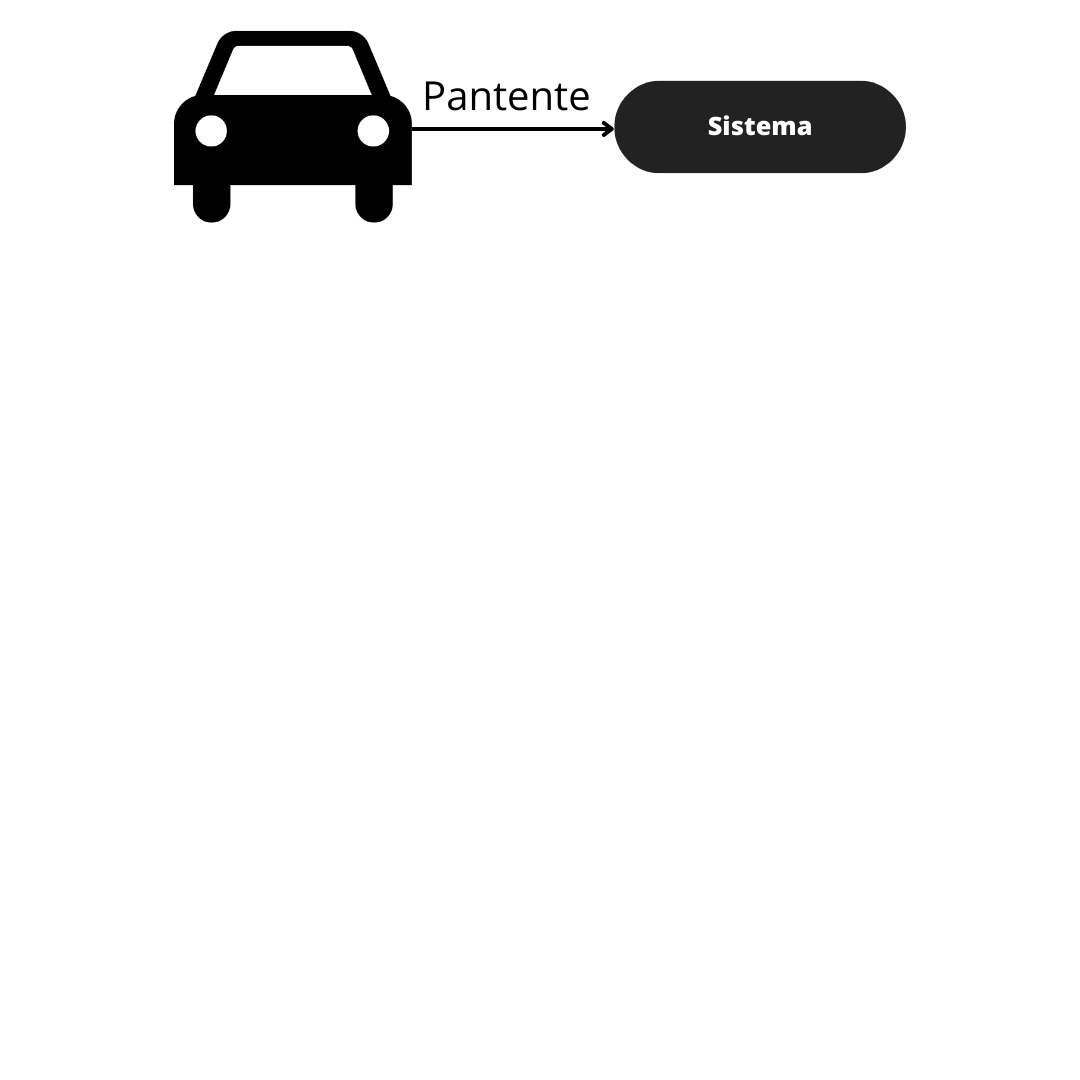
\includegraphics[width=.8\textwidth]{imgs/sistema-base.png}
    \caption[Modelo de caja negra del sistema.]{Idea general del sistema a implementar, en esta versión se toma al bloque de sistema como una caja negra que solo necesita la patente para realizar su tarea.}
    \label{fig:sistema-base}
\end{figure}

De estos requisitos se desprende la forma más general del sistema, que detecta los caracteres del vehículo, permite la identificación del vehículo, y basado en la hora de entrada y salida, calcula el tiempo que estuvo el vehículo. En la Fig. \ref{fig:sistema-base} se observa un modelo de caja negra del sistema.
Existe un gran inconveniente a la hora de obtener el texto de la patente de una imagen y es el tiempo de procesamiento. Es por ello que se utilizará un sensor de distancia para garantizar que existe un objeto.
La versión correspondiente del sistema se puede observar en la Fig. \ref{fig:sistema-completa}.

\begin{figure}[bth]
    \centering
    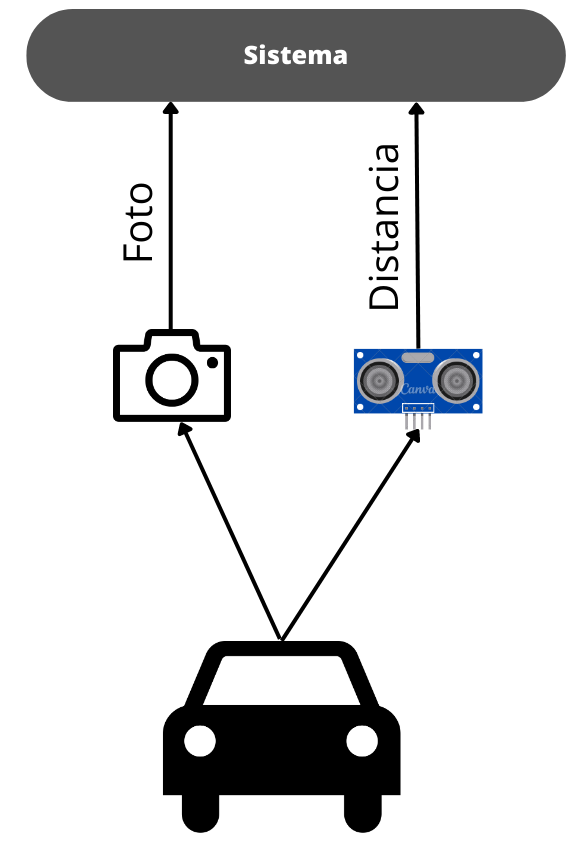
\includegraphics[width=.3\textwidth]{imgs/sistema-con-sensor.png}
    \caption{Sistema con sensor de distancia y cámara.}
    \label{fig:sistema-completa}
\end{figure}

Debido a que los parques de estacionamiento, como los de los supermercados, tienen entradas y salidas diferenciadas, el sistema deberá tener un comportamiento diferente según donde se encuentre.
Es por ello que se implementarán dos algoritmos, uno para manejar las entradas y otro para manejar las salidas.

\section{Algoritmos de entrada y salida}

Una vez establecido como se verá el sistema, se debe definir su comportamiento cuando un vehículo entra o cuando sale.

\subsection{Algoritmo de entrada}

La toma de muestra, es decir, una fotografía, se da cuando el sistema detecta que tiene un objeto a menos de $X$cm. Luego, se procesa la imagen, para obtener la patente en formato de texto.
En caso de encontrar una patente, se almacena la fecha, junto con la patente y la fotografía Fig. \ref{fig:flujo-entrada}.

\begin{figure}[bth]
    \centering
    \begin{subfigure}{.3\textwidth}
        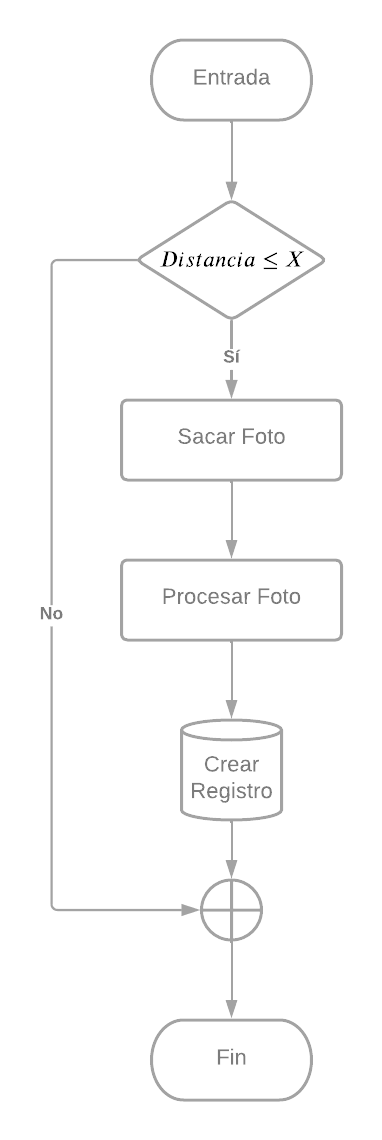
\includegraphics[width=\textwidth]{imgs/flujo-entrada.png}
        \caption{Entrada.}
        \label{fig:flujo-entrada}
    \end{subfigure}
    \hspace{3cm}
    \begin{subfigure}{.3\textwidth}
        \centering
        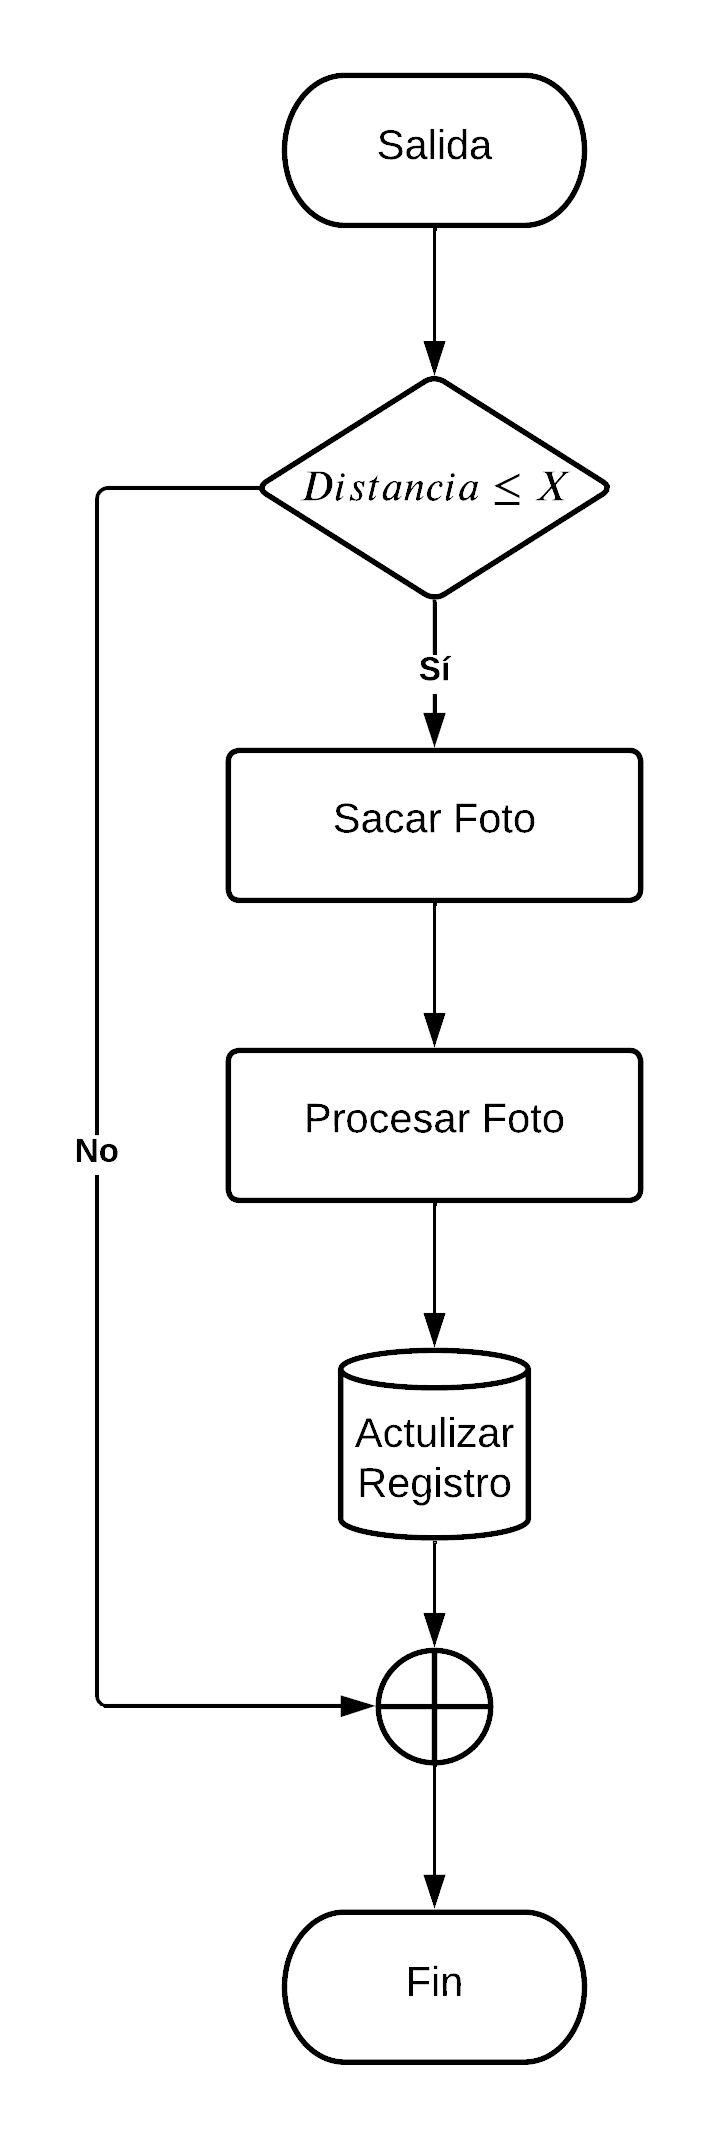
\includegraphics[width=\textwidth]{imgs/flujo-salida.png}
        \caption{Salida.}
        \label{fig:flujo-salida}
    \end{subfigure}
    \caption{Diagramas de flujo para la entrada y la salida de un vehículo del estacionamiento.}
\end{figure}

\subsection{Algoritmo de salida}

El algoritmo de salida es idéntico en la toma de muestra, pero antes de guardar la información de salida (foto y fecha), verifica que exista un registro de entrada correspondiente y se actualiza el mismo Fig. \ref{fig:flujo-salida}.

\subsection{El problema de múltiples establecimientos}

Ambos algoritmos poseen un pequeño inconveniente a la hora de extender el proyecto en más de un recinto. Es por ello que cada barrera se vincula a un lugar, y los registros se buscan y actualizan en función del lugar que tiene asignado cada barrera.

\section{Partes del sistema}

Una vez diseñado y comprendido como está compuesto el sistema a grandes rasgos, es importante entender las partes del mismo y lograr diferenciar que parte del algoritmo se ejecutará en el sistema SL y cuál en el servidor. Para la comunicación del SL con el servidor se optó por utilizar 2 protocolos de comunicación: por un lado HTTP para el envío y actualización de registros de entrada/salida, y MQTT para cambios en la configuración de las barreras, en el capítulo 5 se realizará una explicación de cada protocolo.
En la Fig. \ref{fig:sistema-server-barrera} se observa como interactúan los vehículos con la plataforma, la flecha en rojo se utiliza para destacar el envío de datos por MQTT.

\begin{figure}[bth]
    \centering
    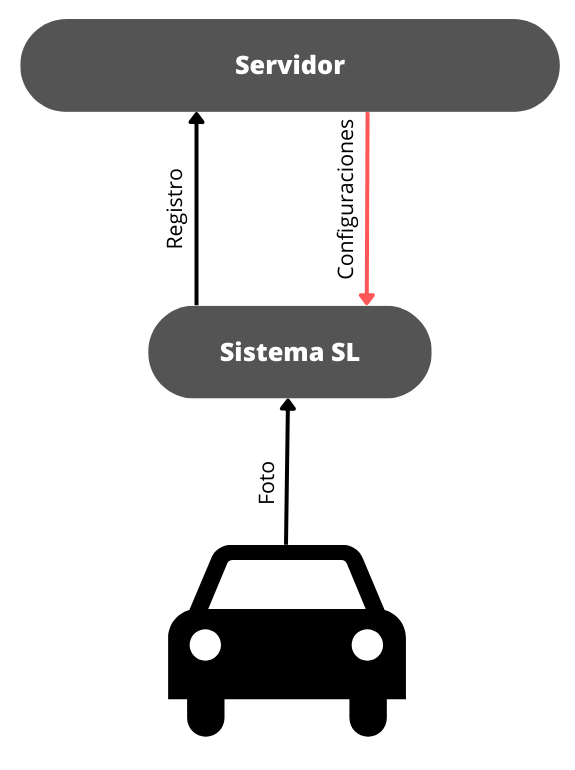
\includegraphics[width=.3\textwidth]{imgs/sistema-server-barrera}
    \caption{Sistema separado en SL y servidor.}
    \label{fig:sistema-server-barrera}
\end{figure}

Esta es la versión que se desarrollará en los capítulos siguientes.

\subsection{Interacción con el cliente}

Debido a que el enfoque del diseño implica un cliente que desea utilizar el sistema se desarrolla una plataforma web para simplificar el manejo de configuración y administración del sistema. En la Fig. \ref{fig:esquema-cliente-servidor-sl} se observa la arquitectura a implementar en el servidor, teniendo en cuenta las interacciones y su manejo entre los sistemas SL y los clientes.
\begin{figure}[bth]
    \centering
    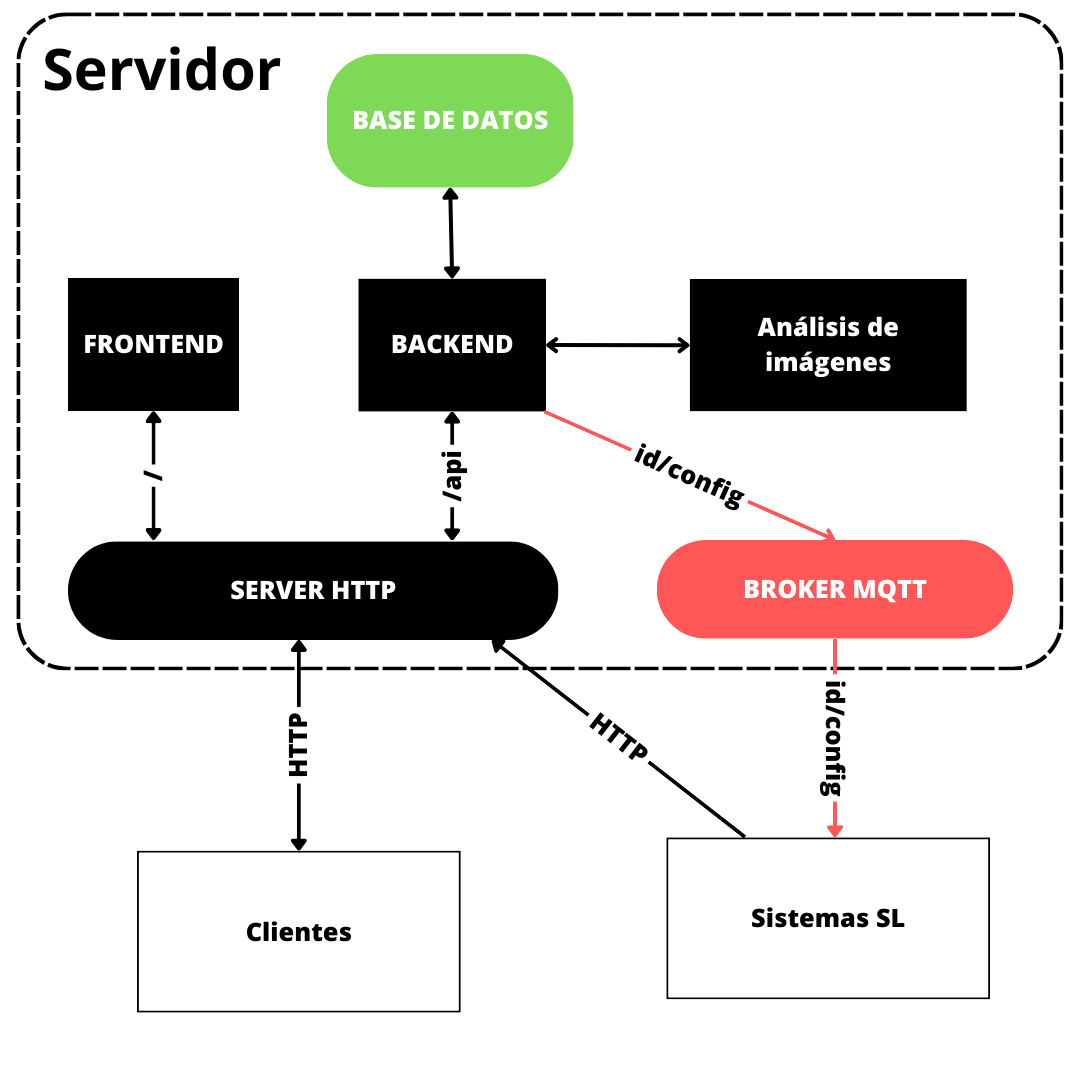
\includegraphics[width=.6\textwidth]{imgs/server-clientes-barreras.png}
    \caption{Esquema de comunicación Cliente-Servidor-SL.}
    \label{fig:esquema-cliente-servidor-sl}
\end{figure}


\chapter{Detección óptica de caracteres}

En este capítulo se explicará que es la detección óptica de caracteres (OCR), y se buscara obtener una idea básica
de los distintos algoritmos que se pueden implementar para
utilizar esta técnica.
Luego se presentará la red convolucional entrenada por
Ankandrew \cite{ankandrew_reconocedor_2023}, con la idea de finalizar en un algoritmo en Python 3
que permita obtener los caracteres de una patente mediante una imagen.

\section{Algoritmos de OCR}

El OCR, por sus siglas en inglés Optical Character
Recognition o en español Reconocimiento Óptico de Caracteres, es una técnica que permite
obtener texto en formato ASCII a partir de una imagen.
Para lograrlo se debe inspeccionar la imagen buscando formas características de los símbolos como los del abecedario.
La tecnología más utilizada en esta ultima decada para realizar el OCR son las Redes Neuronales donde se destacan dos tipos: las redes LSTM, por sus siglas en inglés Long-Short Term Memory, que son una variedad de Redes
neuronales recurrentes, y las CNN por sus siglas en inglés Convolutional Neural Network, o en español Red Neuronal Convolucional.

Si bien el fin último de ambos tipos de red es obtener los caracteres a partir de la imagen, la forma en
la que trabajan difiere significativamente.

\subsection{Redes LSTM}

Las redes LSTM almacenan información de estados anteriores mediante bucles,
lo que les permite realizar predicciones de estados futuros usando información pasada almacenada y la información
del estado actual.
En la Fig. \ref{fig:diagrama-LSTM} se observa un bloque LSTM básico, donde se pueden apreciar las diversas funciones que lo componen. Los bloques $\sigma$ corresponden a las funciones de activación que en general son sigmoides, los bloques $g$ y $h$ son funciones de activación diferentes que en la mayoría de los casos suelen ser tangentes hiperbólicas.
Las señales principales son:
\begin{itemize}
    \item $y^{(t-1)}$: corresponde al estado oculto anterior.
    \item $x^t$: es la entrada del estado actual.
    \item $c^{(t-1)}$: representa el estado previo del bloque.
    \item $c^t$: representa el estado actual del bloque.
    \item $y^t$: corresponde al estado oculto actual.
\end{itemize}

Cada bloque LSTM se puede dividir en tres secciones diferentes que son:

\begin{itemize}
    \item Compuerta de memoria: representado por la funcion $\sigma$, en ella se decide a que información se le debe prestar atención y cuál debe ser ignorada, en otras palabras, es la encargada de ponderar la importancia de la entrada actual respecto a la información pasada.
    \item Compuerta de entrada: esta se obtiene de la multiplicación de las señales $z$ e $i$, es la encargada de actualizar el estado del bloque con la información ponderada de la compuerta de memoria por el vector $z$, cuyos valores se encuentran entre $-1$ y $1$.
    \item Compuerta de salida: aquí se determina el valor actual del estado oculto y queda contenida la información de los estados previos, este valor es utilizado para realizar la predicción de estados futuros.
\end{itemize}
En forma resumida se puede decir que la compuerta de memoria determina que información de los estados anteriores es relevante, la compuerta de entrada decide que información es necesaria añadir al estado actual, y la compuerta de salida determinada el estado oculto actual.
\begin{figure}
    \centering
    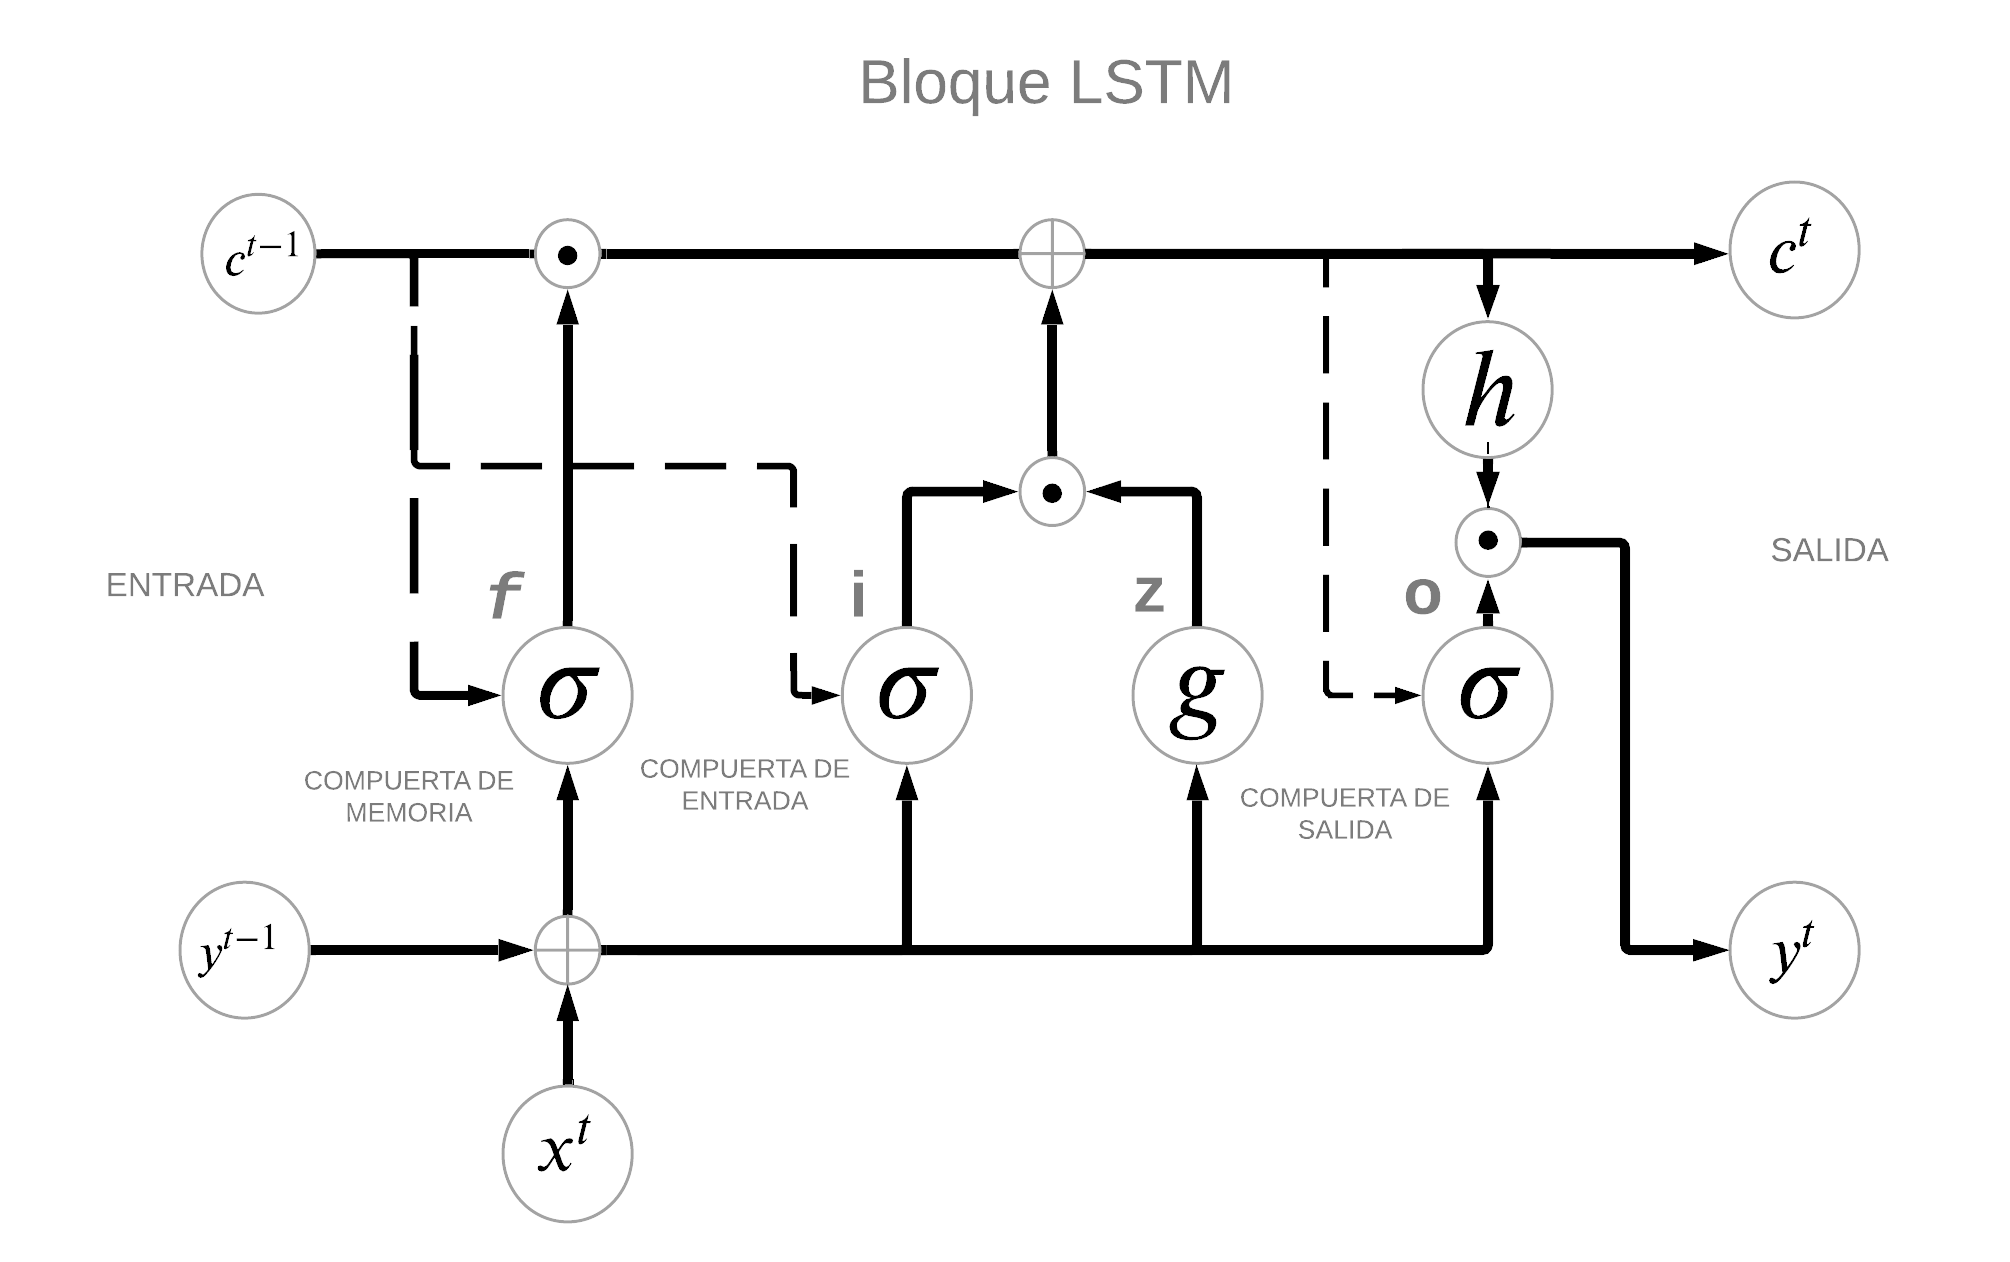
\includegraphics[width=0.5\textwidth]{imgs/diagrama-lstm.png}
    \caption{Diagrama del bloque LSTM.}
    \label{fig:diagrama-LSTM}
\end{figure}

Actualmente, este tipo de redes son las más utilizadas para realizar reconocimiento de caracteres, pero cuentan con la desventaja de un alto costo computacional, lo que desaconsejable su uso en sistemas embebidos.

\subsection{Redes CNN}

La otra alternativa que se puede utilizar son las CNN, que mediante filtros bidimensionales y una serie de capas totalmente conectadas se predice el texto más probable.
Al no requerir almacenar información ni trabajar de forma recursiva, la implementación
de este tipo de redes se puede hacer en equipos con un hardware de menor potencia, menor tamaño y, por consiguiente, menor costo. La mayor desventaja es que la cantidad de caracteres debe estar previamente definido.

Las patentes argentinas han sufrido tres modificaciones a lo largo de los años, que se pueden ver en la Fig. \ref{fig:patentes-arg}. En la actualidad, se pueden encontrar vehículos con las patentes lanzadas en 1994 y 2015. Si se considera un séptimo carácter en las de 1994 como un guion bajo (\_), es posible utilizar una red neuronal del tipo CNN frente a una LSTM.
\begin{figure}
    \centering
    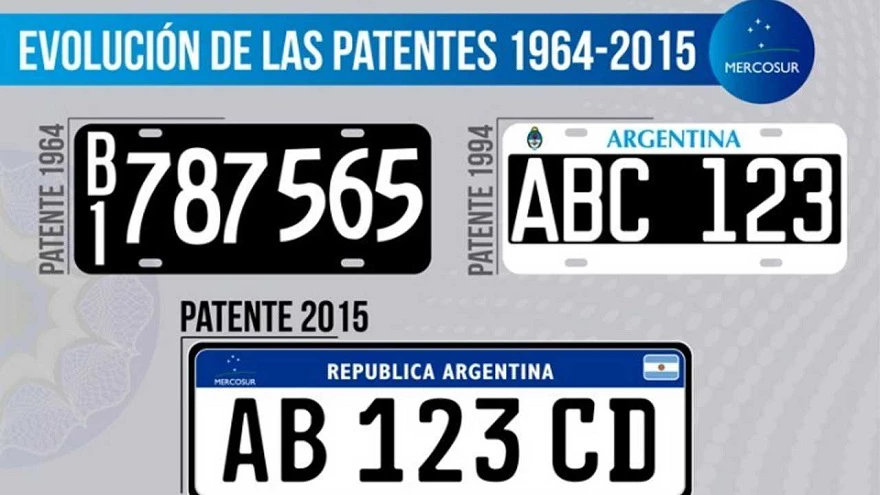
\includegraphics[width=0.5\textwidth]{imgs/patentes-arg.png}
    \caption{Evolución patentes Argentinas a lo largo de los años.}
    \label{fig:patentes-arg}
\end{figure}


\section{¿Qué es una red neuronal?}

Se entiende como red neuronal a un algoritmo computacional que intenta imitar el cerebro humano, en otras palabras, es un algoritmo de computación compuesto por un gran número de elementos simples que se
encuentran interconectados, los cuales procesan la información por medio de estados dinámicos, respondiendo a entradas externas, que permite realizar diversas tareas.
En este caso el trabajo se centrará en la tarea de clasificación de datos.
Debido a la semejanza que existe entre los algoritmos de Deep Learning \cite{ibm_que_nodate} (algoritmos de aprendizaje profundo) y el cerebro humano, a la unidad fundamental de estos sistemas se la denomina neurona.


\subsection{La neurona}

La neurona es la unidad fundamental dentro de la red, y su nombre viene de la similitud que existe entre este elemento y una neurona humana, esto se puede apreciar en Fig. \ref{fig:comparativa-neuronas}. La tarea de la neurona es procesar la información que le entra para producir un valor de salida, a este proceso se lo conoce como sinapsis.

\begin{figure}
    \centering
    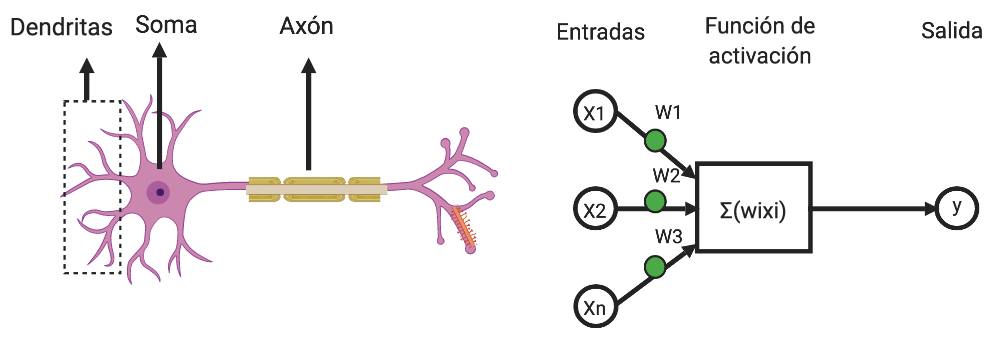
\includegraphics[width=1\textwidth]{imgs/comparacion-neurona-red.png}
    \caption{Comparación neurona con neurona artificial.}
    \label{fig:comparativa-neuronas}
    %https://futurelab.mx/redes%20neuronales/inteligencia%20artificial/2019/06/25/intro-a-redes-neuronales-pt-1/
\end{figure}

La sinapsis entre neuronas es una suma ponderada que puede ser expresada como $y =W^T \cdot X + b$ donde $y$ es el valor de salida de la neurona,
$W$ representa los pesos de la neurona y se define como un vector columna de dimensión $N$, $b$ es un bias y $X$ es el vector columna de dimensión $N$. Si bien la neurona es muy útil, sola no es de mucha utilidad, es por ello que a los arreglos en paralelo de neuronas se los denomina capa, a la conexión de capas de neuronas simples se las denomina capas totalmente conectadas, ya que toda la información de la capa anterior se envía a la capa siguiente.

\section{Redes neuronales}

A la hora de resolver problemas más complejos es usual necesitar más de una capa, es por ello que se interconectan para formar una red neuronal en la Fig. \ref{fig:esquema-redes} se observa una red con varias capas.

\begin{figure}
    \centering
    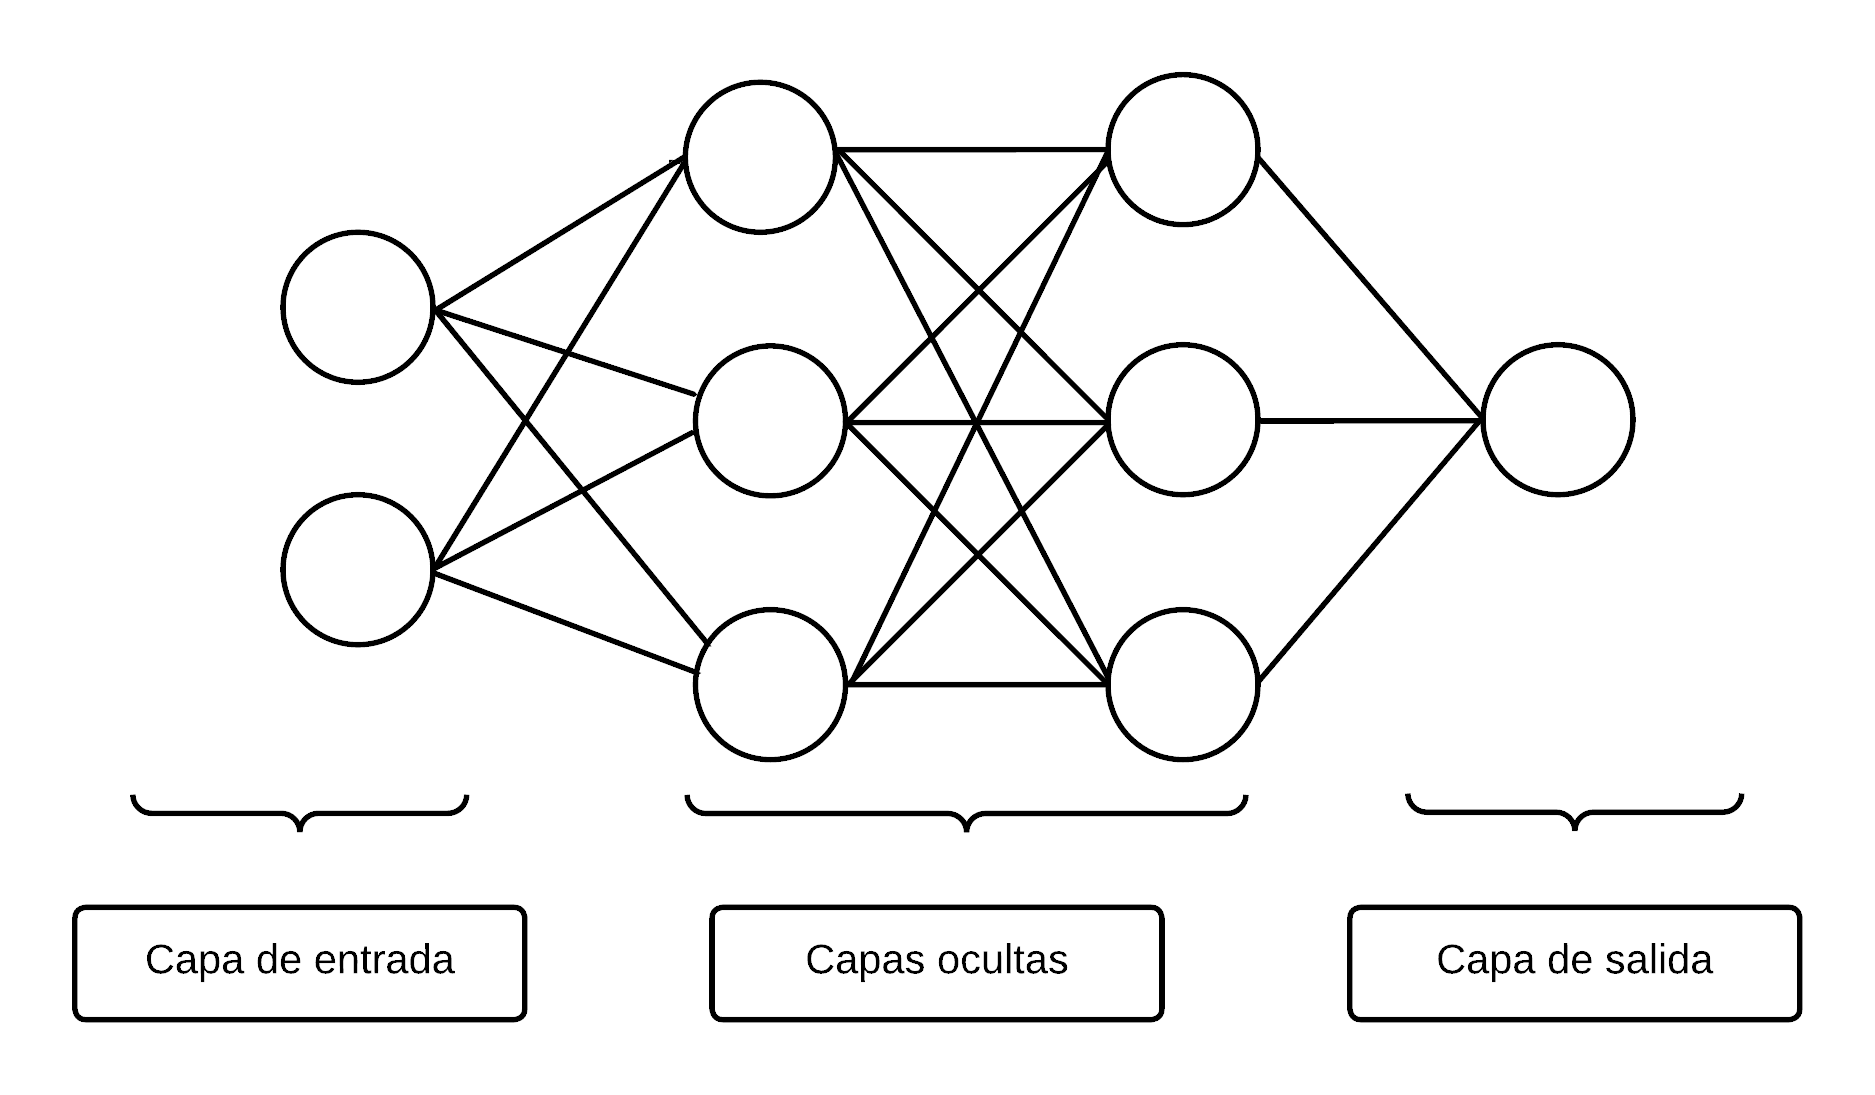
\includegraphics[width=0.6\textwidth]{imgs/Redes-esquema.png}
    \caption{Esquema simplificado de una red neuronal.}
    \label{fig:esquema-redes}
\end{figure}

Debido a que en esencia el proceso que realiza la neurona es una transformación lineal, al interconectar capas la resultante sigue siendo una transformación lineal.
Este problema de linealidad se soluciona aplicando una transformación no lineal, la cual se suele llamar función de activación,
luego de que la información es procesada por la neurona, obteniendo $y= f(W^T X + b)$. Las funciones de activación más conocidas se pueden observar en la Fig. \ref{fig:funciones-activacion}.

\begin{figure}
    \centering
    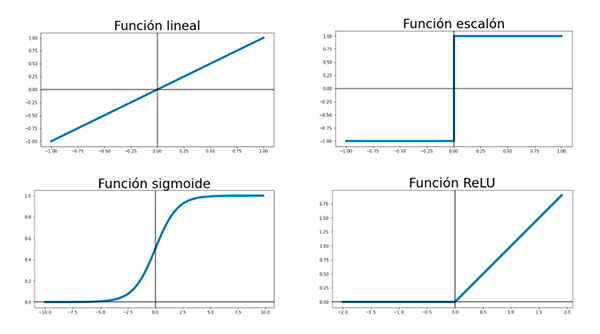
\includegraphics[width=1\textwidth]{imgs/Funciones-de-activacion.jpg}
    \caption{Funciones de activación más comunes.}
    \label{fig:funciones-activacion}
\end{figure}

En resumen una red funciona de la siguiente manera, se realiza la multiplicación de la entrada por los pesos de la red, luego los resultados son ingresados a la función de activación para quitar las linealidades. Posteriormente esta información se pasa a la capa siguiente y se realiza el mismo proceso. Esto se repite hasta llegar a la capa de salida donde, en tareas de clasificación, se suelen colocar tantas neuronas como salidas posibles.

\section{Redes neuronales de convolución}

Si bien, hasta ahora se han analizado solo las capas totalmente conectadas existen una gran cantidad de capas diferentes, para este trabajo se dará una breve introducción a las redes de convolución o CNN.

La función principal de las capas de convolución es poder extraer información de una imagen, es por ello que nace la semejanza entre las CNN y la corteza visual de los animales.
Este tipo de redes poseen características que las hacen únicas, por lo que se estudiarán las partes que la componen.
En la Fig. \ref{fig:esquema-CNN} se observa un esquema de la misma.
\begin{itemize}
    \item Capa convolucional: capa principal de las CNN, sus parámetros son básicamente filtros entrenables de dimensiones determinadas por el
          usuario, que realiza una multiplicación punto a punto recorriendo toda la imagen y produciendo un mapa de activación bidimensional, es decir, otra imagen. En la
          Fig. \ref{fig:esquema-capa-convolucional} se ve el funcionamiento de esta capa. Cada uno de los filtros se activarán según la característica que aprenda la red.
    \item Capa de agrupación: se coloca entre las capas de convolución, toma los mapas de características producidos por la capa de
          convolución y los agrupa en una imagen. En esta capa se produce una reducción de la dimensión, lo que reduce la complejidad para evitar el sobreajuste de los parámetros.
    \item Función de activación.
    \item Capa de aplanamiento o Flatten: Antes de pasar las salidas de las capas convolucionales se produce un aplanamiento de las imágenes, esta capa transforma las imágenes o matrices de dimensión $N \times N$ en un vector columna $2NM$, donde $M$ es la cantidad de filtros de la capa anterior.
    \item Capa completamente conectada: Se encargan de procesar la información de los filtros para obtener la cantidad de salidas esperadas.
\end{itemize}

Si bien la descripción de las capas de convolución, agrupación y función de activación se realizaron de forma separa, se suelen implementar juntas, ya que es común tener varias capas de convolución conectadas en serie, permitiendo extraer información más especifica de la red.

\begin{figure}
    \centering
    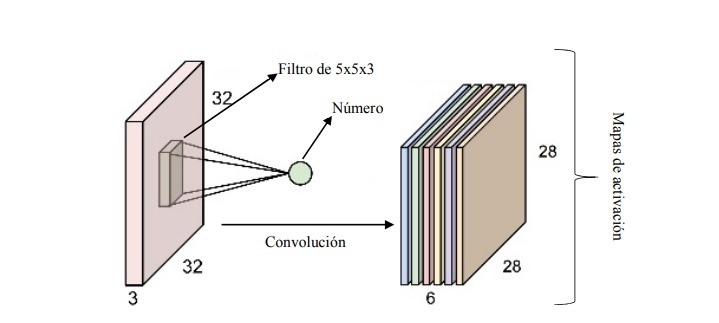
\includegraphics[width=1\textwidth]{imgs/capa-convolucional.jpeg}
    \caption{Esquema de funcionamiento de una capa convolucional.}
    \label{fig:esquema-capa-convolucional}
\end{figure}
\begin{figure}
    \centering
    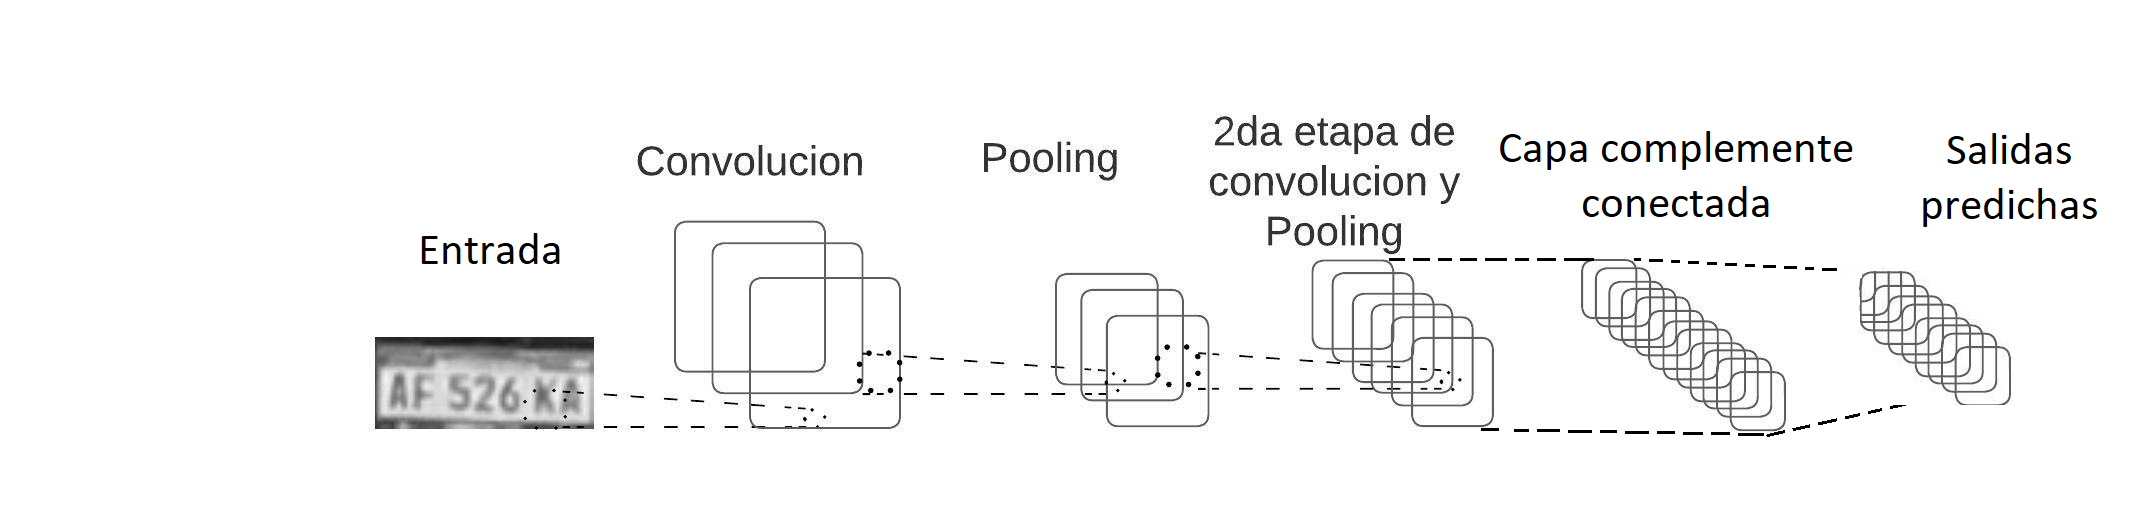
\includegraphics[width=1\textwidth]{imgs/CNN-completa.png}
    \caption{Ejemplificación de una red neuronal de convolución.}
    \label{fig:esquema-CNN}
\end{figure}

\subsection{Convolución en 2D}

La convolución bidimensional es similar al caso conocido en 1D, pero en este caso se desplaza una submatriz de un tamaño predefinido, comúnmente denominado kernel, por la matriz o imagen de entrada.

Se define kernel a la respuesta de un sistema discreto, el cual es de dimensión $2k \times 2k$, donde $k$ es un
valor establecido arbitrario (usualmente se utilizan matrices de $3 \times 3$ o $5 \times 5$) que define cuántos valores de la muestra habrá.

Se define a $h[n,m]$ como un filtro de dimensión $(2k + 1) \times (2k + 1)$ e $I$ una imagen a escala de grises, donde cada punto de coordenadas $(i,j)$ es el
resultado de la convolución entre $h$ e $I$ dado por

\begin{equation}
    O(i,j)= \sum_{u=-k}^{k} \sum_{v=-k}^{k} h[u,v]I[i-u,j-v]
\end{equation}

Esta operación consiste en filtrar una subimagen de dimensión $(2k+1)\times(2k+1)$ en la imagen $I$ original para cada pixel centrado en dicha imagen, calculando la operación de convolución y dando como resultado un pixel de la imagen de salida $O$.
este proceso
\subsection{Capa de agrupación}

La capa de agrupación o pooling se encarga de reducir el tamaño de la imagen ejecutando una función a una submatriz de $n \times n$ de la imagen pasando de tener $n^2$ elementos a un elemento, las funciones de polling más utilizadas son:

\begin{itemize}
    \item MaxPooling: se queda con el valor máximo de la submatriz.
    \item AveragePooling: calcula la media de los elementos.
\end{itemize}

Otra forma de entender a la capa de pooling es un submuestreo de la imagen de salida de la capa de convolución que devuelve el valor más significativo.

En la Fig. \ref{fig:ejemplo-mp} se puede apreciar el comportamiento de una capa de maxpooling. Luego de la capa de convolución, se divide la matriz
en pequeñas matrices de $2 \times 2$ y se extrae el valor más representativo de cada submatriz, reduciendo la matriz de un tamaño de $5 \times 5$ a una de $3 \times 3$, en este caso.
\begin{figure}
    \centering
    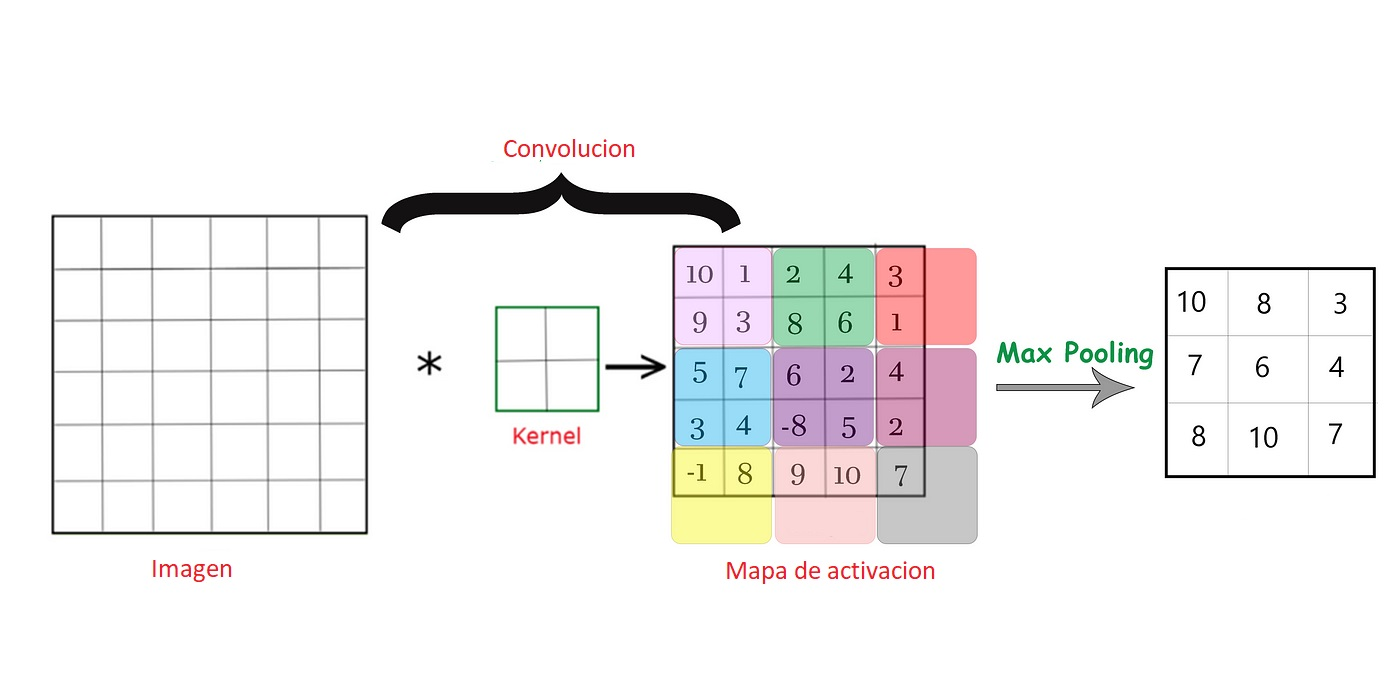
\includegraphics[width=1\textwidth]{imgs/ej-maxpooling.jpg}
    \caption{Ejemplo de funcionamiento de Maxpooling.}
    \label{fig:ejemplo-mp}
\end{figure}

\subsection{Técnica de Batch-Normalization}

La técnica de Batch-Normalization se utiliza para reducir la covarianza de los datos de entrada. Esto se realiza normalizando los datos de entrada en un rango de 0 a 1 evitando trabajar con números grandes. Si bien este proceso se suele realizar con los datos de entrada, es útil realizarlo entre capas antes de la función de activación para trabajar siempre con datos normalizados, lo que permite un ajuste de parámetros más simple. Finalmente antes de pasar a la capa siguiente se aplica la función de activación.

\section{CCN-OCR}

Para este trabajo se utilizó una CNN diseñada y entrenada por Ankadrew, cuya arquitectura se puede ver en Fig. \ref{fig:arquitectura-cnn-ocr}. De la arquitectura de la red se destaca la capa de Global Average Pooling, la cual remplaza a la capa de aplanamiento y calcula la media por cada imagen de salida de la capa anterior, produciendo un valor por cada imagen [incluir figura de la diferencia de una capa de Flatten y un global average pooling].
\begin{figure}
    \centering
    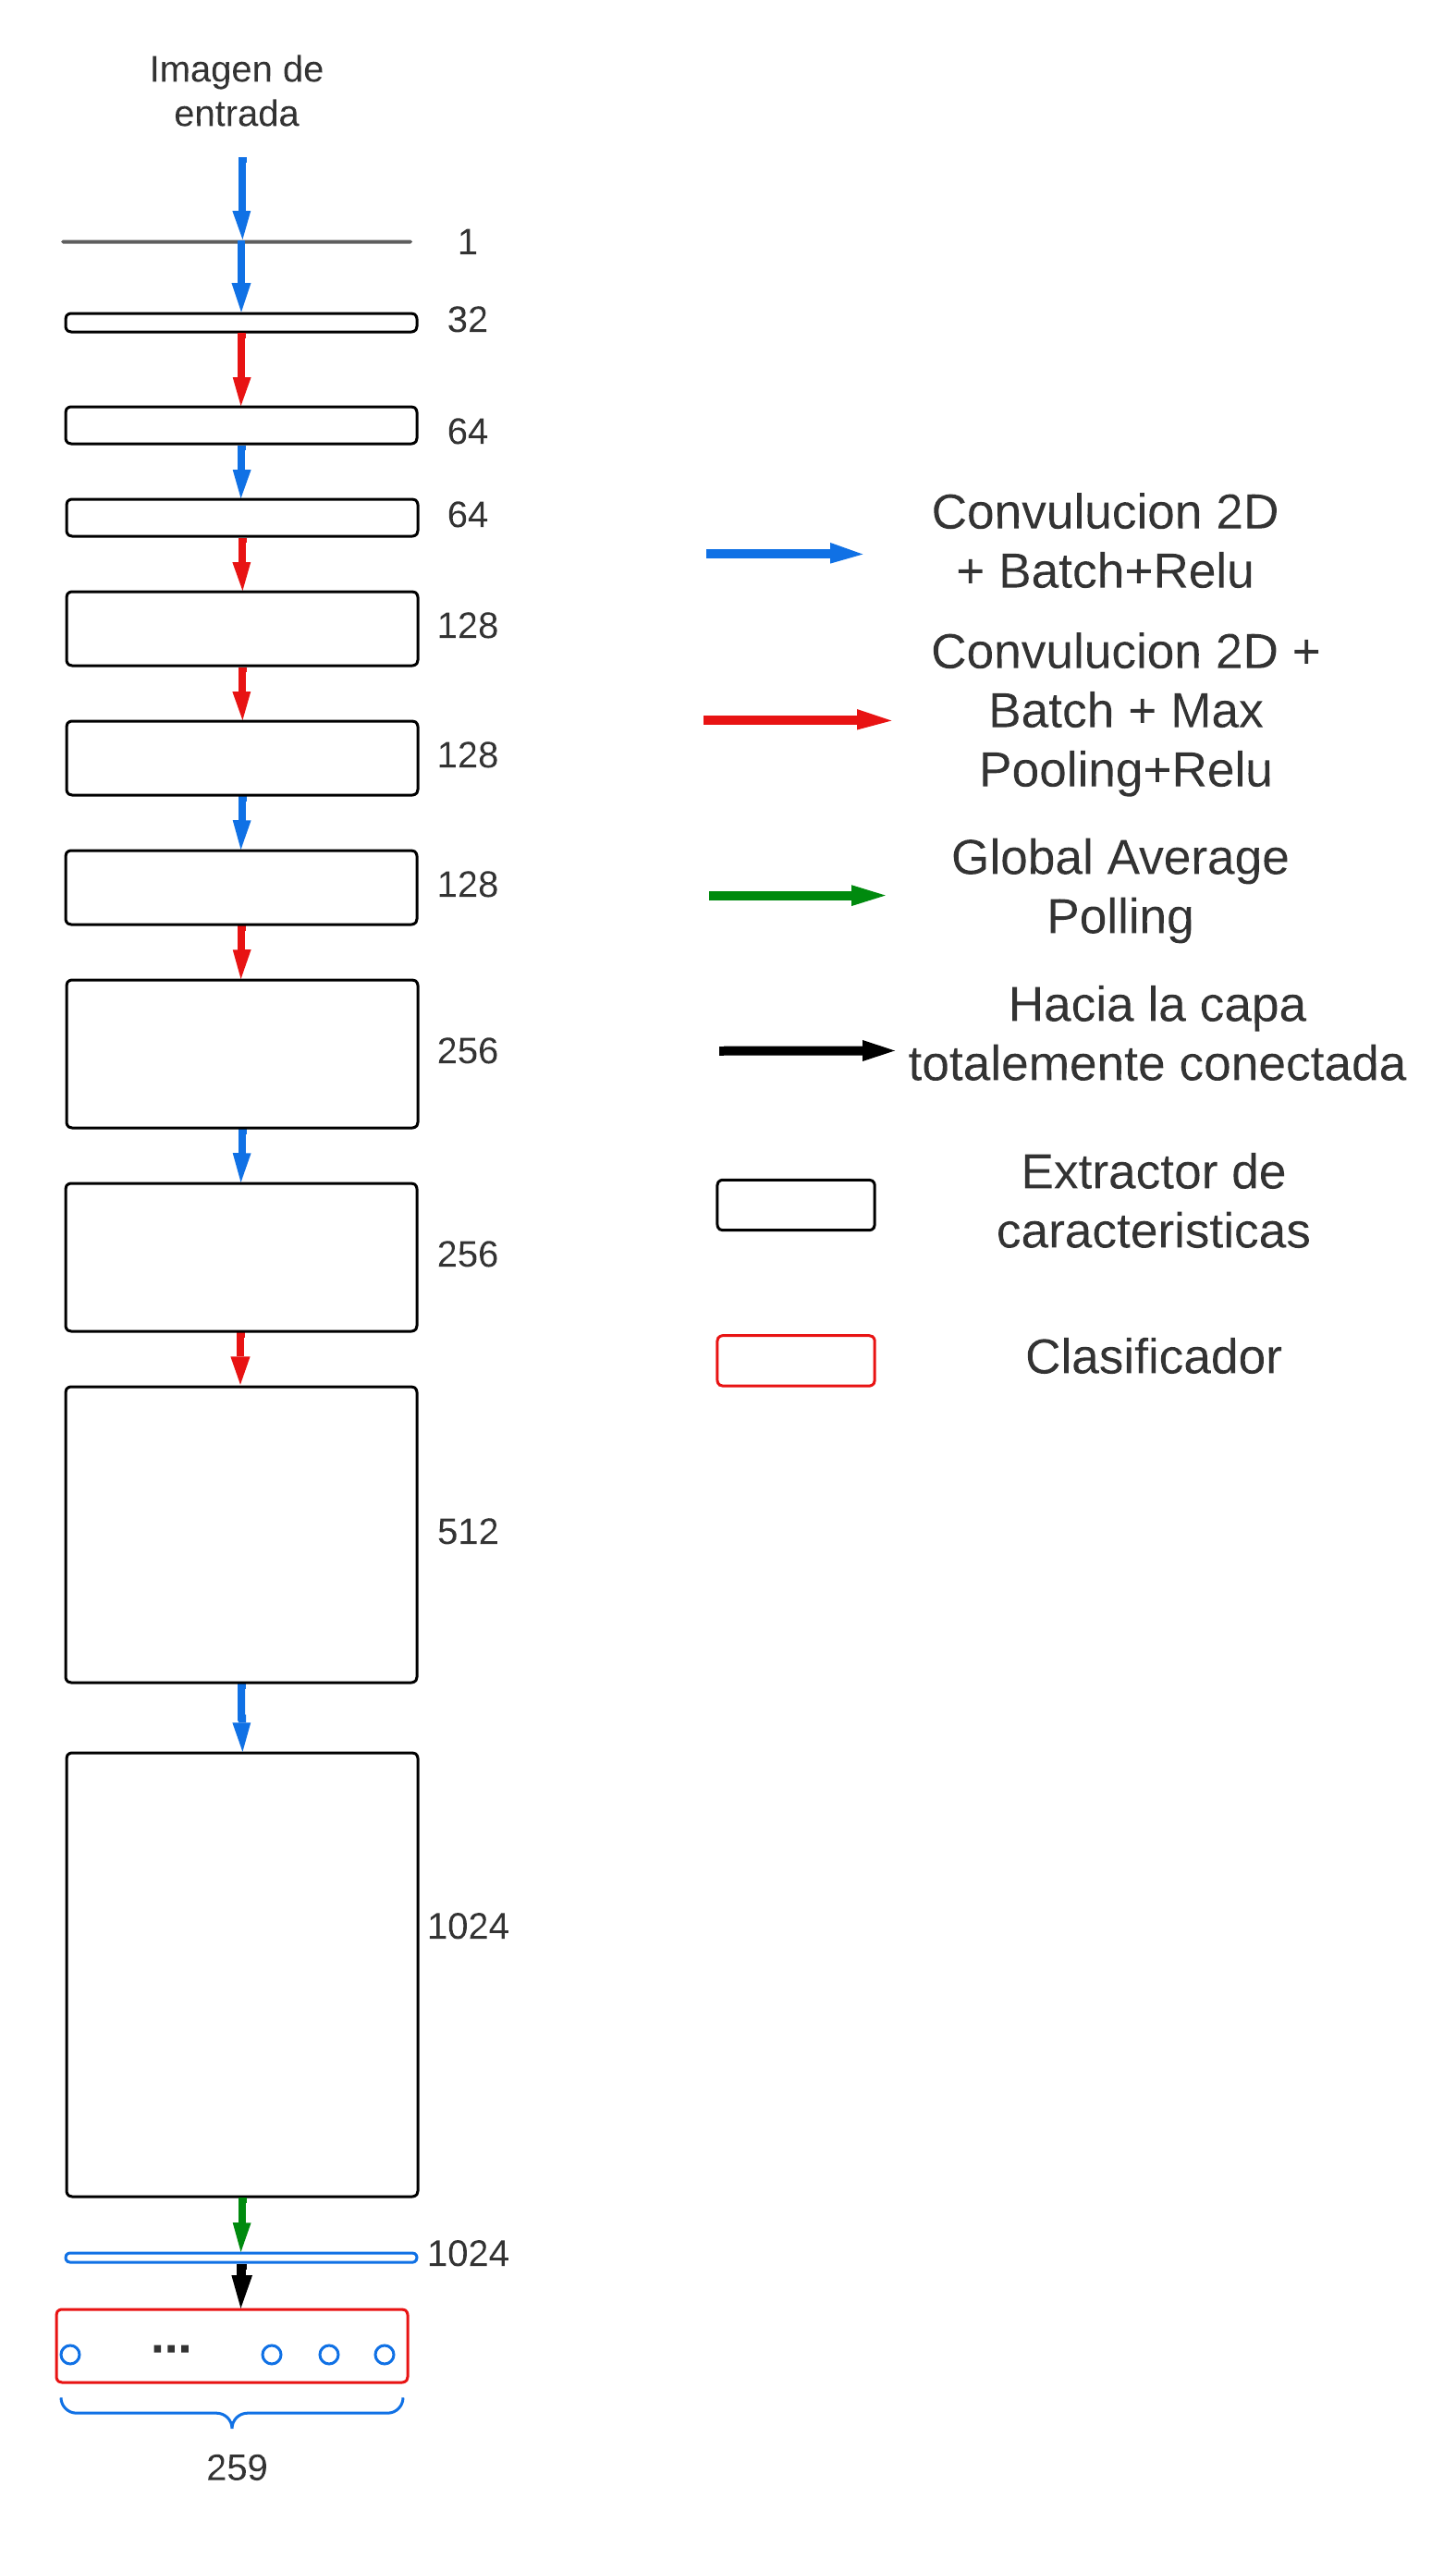
\includegraphics[width=.4\textwidth]{imgs/cnn-ocr.png}
    \caption{Arquitectura de la CNN-OCR.}
    \label{fig:arquitectura-cnn-ocr}
\end{figure}

Otro elemento a destacar de la red son las siete capas densas conectadas en paralelo, debido a que, como se anticipó en secciones anteriores, las patentes poseen siete caracteres. En esencia cada capa densa es idéntica, solo se diferencian sus pesos que son aprendidos durante el entrenamiento de la misma. Cada capa posee en total treinta y siete caracteres de salida, esto surge de las veintiseis letras del abecedario, los diez números del 0 al 9 y el símbolo de guion bajo (\_) utilizado en el caso de las patentes antiguas que solo poseen seis caracteres.

Como aclaración para el resto del trabajo, se referirá a esta red como CNN-OCR.

\subsection{Requerimientos}

Si bien la CNN es muy útil para la tarea a resolver, posee una serie de requisitos previos en la imagen de entrada. Según el autor, la CNN
necesita como entrada una imagen de la patente en blanco y negro de dimensiones $70 \times 140$ pixeles.
Por lo que es necesario realizarle un tratamiento previo a las imágenes antes de ingresarlas por la CNN-OCR. El tratamiento necesario
se puede observar en la Fig. \ref{fig:Comparativa-imagenes}. Entonces existen tres pasos previos luego de sacar
la captura antes de ingresarla a la CNN-OCR:

\begin{enumerate}
    \item Obtener un recorte de la patente.
    \item Transformar la imagen a escala de grises.
    \item Redimensionar la imagen al tamaño requerido.
\end{enumerate}
\begin{figure}
    \centering
    \begin{subfigure}[b]{0.49\textwidth}
        \centering
        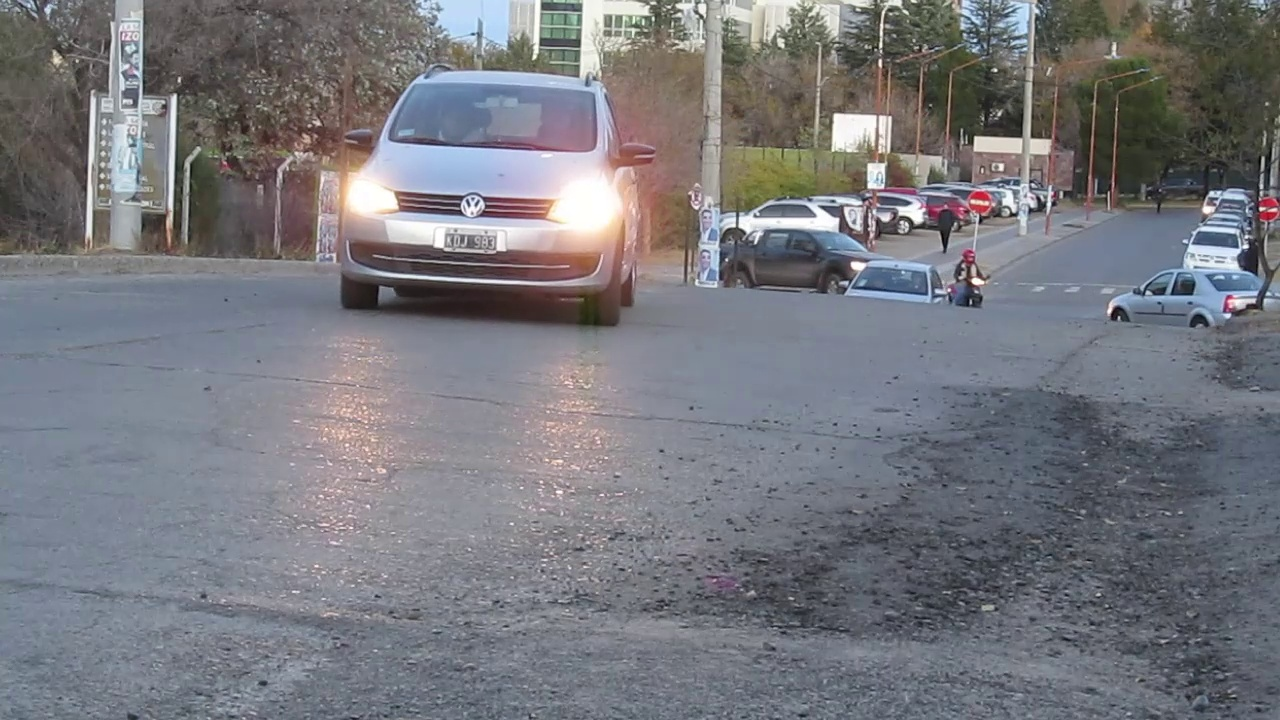
\includegraphics[width=\textwidth]{imgs/imagen-obtenida.jpg}
        \caption{Imagen obtenida por la cámara.}
        \label{fig:imagen-obtenida}
    \end{subfigure}
    \hfill
    \begin{subfigure}[b]{0.49\textwidth}
        \centering
        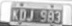
\includegraphics[width=0.7\textwidth]{imgs/imagen-requerida.jpg}
        \caption{Imagen requerida por la CNN-OCR.}
        \label{fig:imagen-requerida}
    \end{subfigure}
    \caption{Ejemplo de imagen obtenida e imagen requerida por la CNN-OCR.}
    \label{fig:Comparativa-imagenes}
\end{figure}

\subsubsection*{Obtención del recorte de la patente}

Debido a la importancia de esta etapa y a su complejidad, se realiza una explicación extendida, con la finalidad de tener una mejor comprensión del funcionamiento del proceso de recorte necesario para que la CNN-OCR pueda funcionar de manera óptima. Siguiendo la recomendación del autor de CNN-OCR, se utilizó una red complementaria que detecta la ubicación de la patente y luego realiza el recorte. La red recomendada para esta tarea es la Yolo (You Only Look Once) en su versión 4 o YoloV4 \cite{bochkovskiy_yolov4_2020}.

El modelo de la YoloV4 es un sistema de código abierto el cual se centra en la detección de objetos. Utiliza una arquitectura Darknet \cite{noauthor_darknet_nodate}, escrita en C, que se puede ver en la Fig.\ref{fig:funcionamiento-yolo}.
Una de las principales características de esta arquitectura es la forma en que realiza el proceso de detección y posterior clasificación. La red se puede entender como tres partes diferentes que, para mantener la nomenclatura de la propia arquitectura, no fueron traducidas y se mantendrán en inglés. Estas partes son:

\begin{itemize}
    \item Head: es la parte encargada de reconocer objetos, básicamente busca una región en la que pueda haber un objeto, sin distinguir cuál sea. Se utilizan dos etapas de detectores, la primera utiliza subimágenes de tamaño fijo, y la otra varía el tamaño de las subimágenes para adecuarse mejor al tamaño de cada objeto.
    \item Backbone: es una arquitectura de deep learning que actúa como extractor de características. Es, en esencia, un modelo de clasificación. Se encarga de tomar las ubicaciones obtenidas por el Head y clasificar sí son o no los objetos requeridos. Es la única parte de la red que se modifica y entrena dependiendo el entorno en que se desea utilizar.
          En el caso de este trabajo el Backbone fue entrenado por el mismo autor de la CNN-OCR para que reconozca patentes argentinas \cite{ankandrew_localizador_2021}.
    \item Neck: su funcionalidad es tomar mapas de característica de diferentes partes del Backbone y agregarle características, para facilitar la clasificación de los objetos.
\end{itemize}

Debido a que la Darknet está escrita en C es necesario compilar la misma, esto se hizo siguiendo los pasos del repositorio de AlexeyAB \cite{alexey_yolo_2023}.


\begin{figure}
    \centering
    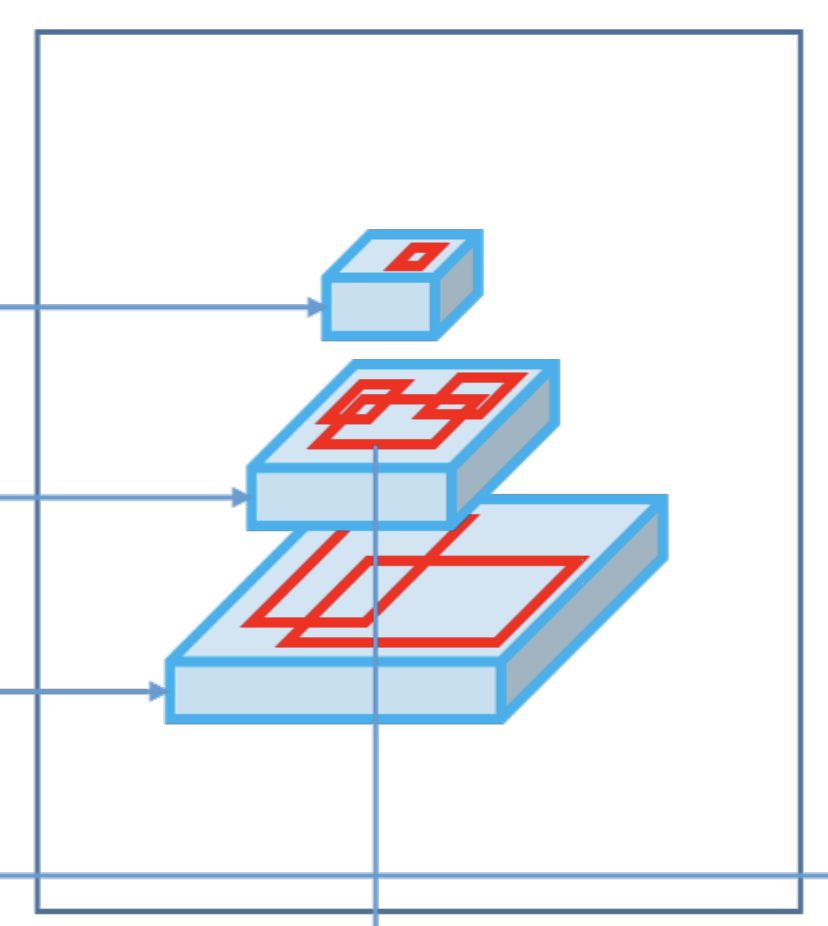
\includegraphics[width=0.5\textwidth]{imgs/funcionamiento-yolo.png}
    \caption{Funcionamiento del proceso de detección de la YoloV4 \cite{bochkovskiy_yolov4_2020}.}
    \label{fig:funcionamiento-yolo}
\end{figure}

\subsubsection*{Transformación a escala de grises}

El proceso de conversión a escala de grises se puede hacer de diversas maneras. La forma más utilizada es realizar un promedio de las capas de color Rojo ($R$), Verde ($G$), Azul ($B$) quedando descripto por la eq. \ref{eq:gray-mean}. Existe otra forma utilizando un promedio ponderado para compensar la sensibilidad relativa del ojo humano la cual se puede observar en la eq. \ref{eq:gray-human}. En la Fig. \ref{fig:comparacion-grises} se observa que el método de escala de grises teniendo en cuenta la sensibilidad del ojo humano obtiene un mejor resultado.

\begin{equation}
    \label{eq:gray-mean}
    I = \frac{R + G + B}{3}
\end{equation}

\begin{equation}
    \label{eq:gray-human}
    I = 0.2989R + 0.587G + 0.114B
\end{equation}

\begin{figure}
    \centering
    \begin{subfigure}[b]{0.3\textwidth}
        \centering
        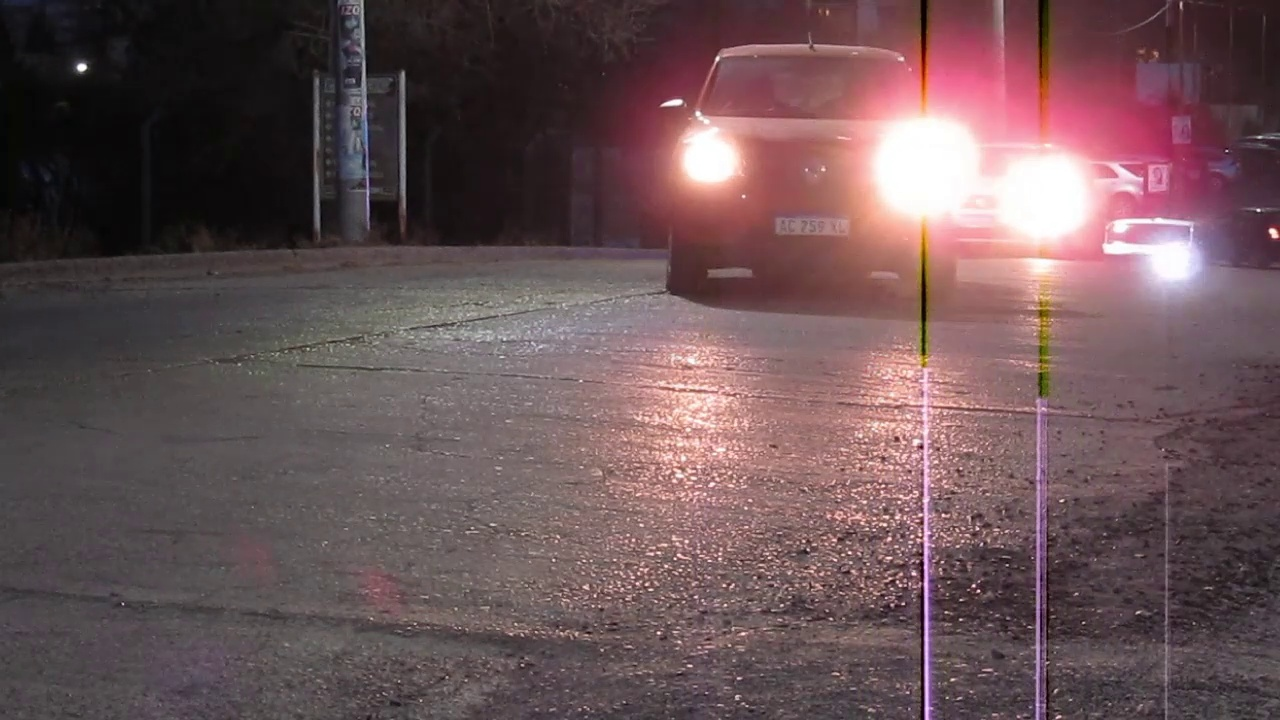
\includegraphics[width=\textwidth]{imgs/escala-grises-original.jpg}
        \caption{Imagen original.}
    \end{subfigure}
    \hfill
    \begin{subfigure}[b]{.3\textwidth}
        \centering
        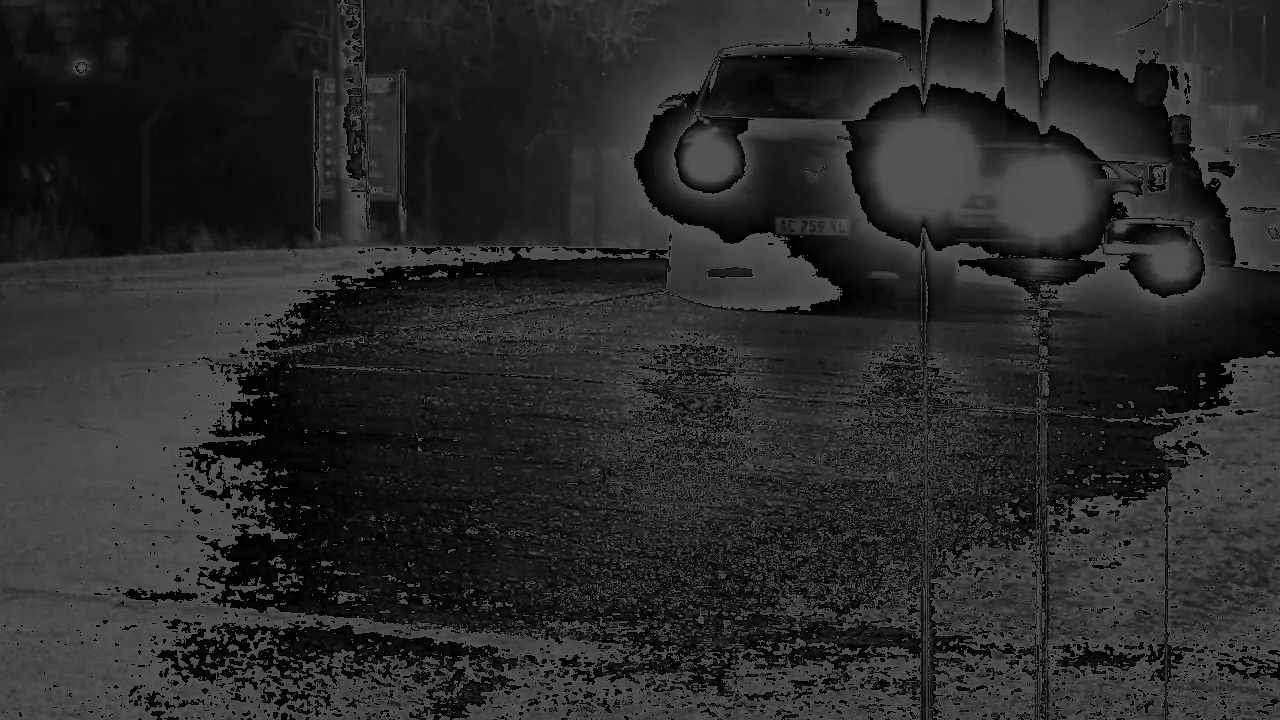
\includegraphics[width=\textwidth]{imgs/escala-grises-promedio.jpg}
        \caption{Promedio.}
    \end{subfigure}
    \hfill
    \begin{subfigure}[b]{.3\textwidth}
        \centering
        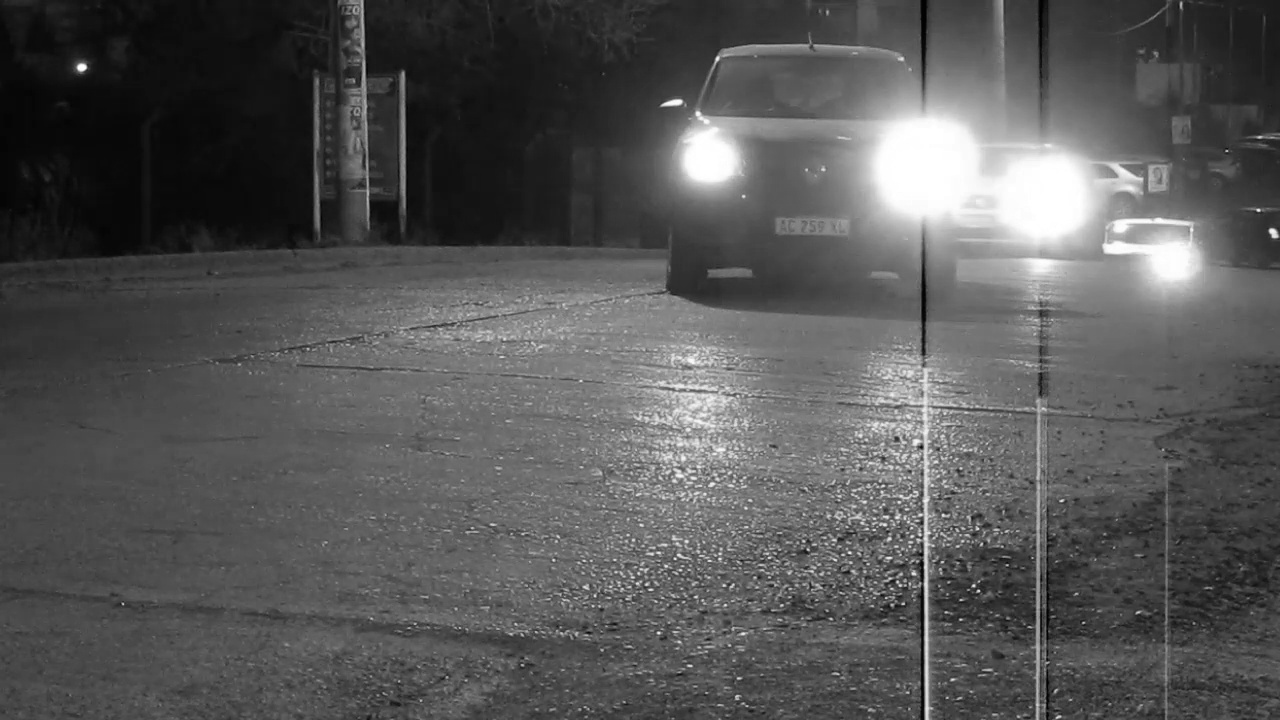
\includegraphics[width=\textwidth]{imgs/escala-grises-sensibilidad.jpg}
        \caption{Promedio ponderado.}
    \end{subfigure}
    \hfill
    \caption{En a) se observa la imagen original, mientras que en b) y c) la imagen convertida a escala de grises por los diferentes métodos.}
    \label{fig:comparacion-grises}
\end{figure}

\subsubsection*{Redimensionamiento de la imagen}

Para redimensionar la imagen se utiliza una interpolación bilineal la cual no se explicará en este trabajo debido a la complejidad del algoritmo.

\section{Implementación del algoritmo en Python 3}

Para la implementación del algoritmo se utilizó el lenguaje Python 3, ya que cuenta con una gran cantidad de librerías necesarias para el funcionamiento del sistema completo. La descripción general del algoritmo se puede observar en Fig. \ref{fig:algoritmo-ocr}.

\begin{figure}
    \centering
    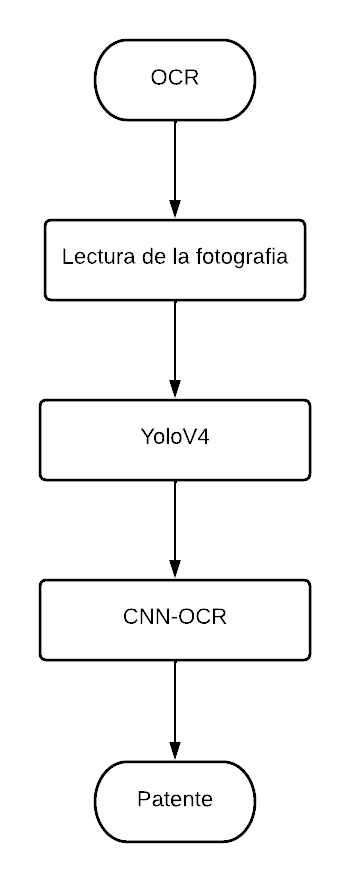
\includegraphics[width=.25\textwidth]{imgs/flujo-algoritmo-ocr.png}
    \caption{Algoritmo general de OCR.}
    \label{fig:algoritmo-ocr}
\end{figure}


\begin{figure}
    \centering
    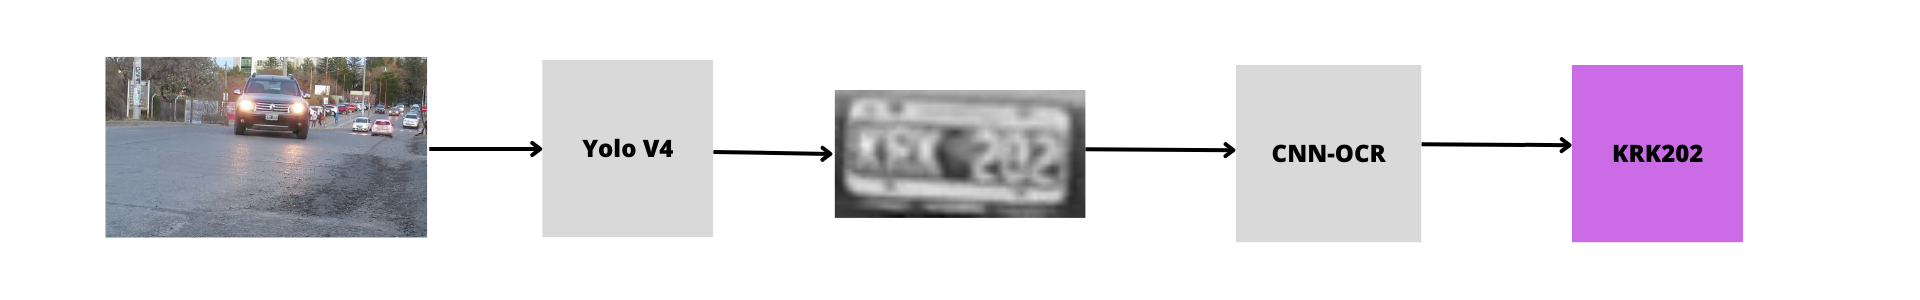
\includegraphics[width=\textwidth]{imgs/pic-to-text.png}
    \caption{Flujo de una fotografía hasta obtener el texto de la patente.}
    \label{fig:pic-to-text}
\end{figure}


La lectura u obtención de una fotografía se realizó mediante OpenCV \cite{opencv_opencv_2023} ya que permite utilizar una gran variedad de fuentes tales como cámaras y archivos. Luego se procesa mediante la YoloV4, que devuelve la ubicación relativa de la patente en la imagen en un archivo de texto plano para, posteriormente, leer el archivo de texto, junto con las dimensiones de la imagen y poder obtener la patente recortada. Antes de pasar el recorte a la CNN-OCR se la cambia a escala de grises y se la lleva al tamaño de $70 \times 140$ utilizando una interpolación lineal y se normalizan los valores de la imagen entre 0 y 1 usando OpenCV. Finalmente se procesa la imagen por la CNN-OCR obteniendo la patente en texto. En capítulos posteriores se explicará en mayor detalle que sucede con la imagen, y la patente obtenida (Fig. \ref{fig:pic-to-text}).


\subsection{Prueba de rendimiento}

Con la finalidad de dimensionar los tiempos de procesamiento del algoritmo de OCR, se procesaron diez imágenes y luego, se calculó el promedio para obtener el tiempo promedio por imagen en diferentes sistemas. Los resultados se encuentran en Tab. \ref{tab:ocr}.
Luego de analizar los tiempos obtenidos, se observa que la Raspberry Pi tarda demasiado en procesar una imagen, mientras que los otros sistemas poseen tiempos similares.
\begin{table}
    \centering
    \begin{tabular}{ccccc}
        \toprule
                   & Raspberry Pi 3b+ & Jetson TX1 & I5-11600K & I5-1135G7 \\
        \midrule
        Tiempo [s] & 85.78            & 6.15       & 1.05      & 1.20      \\
        \bottomrule
    \end{tabular}
    \caption{Tiempos obtenidos del procesamiento de diez imágenes.}
    \label{tab:ocr}
\end{table}




\chapter{Implementación de hardware}
En este capítulo se detallará cuál es el hardware utilizado para el desarrollo del sistema de acceso, se indicarán cuáles
son los requisitos mínimos que deben satisfacerse para que el sistema cumpla las características solicitadas, como
también se indicarán los sensores y equipos auxiliares usados junto con otras posibles opciones encontradas y las
razones por las que estas fueron descartadas.


\section{Estado actual del sistema de acceso por barreras}

\subsection{Sistemas tradicionales}

Hoy en día el sistema de uso de barreras para el control de ingreso y egreso a distintos recintos suelen generar molestias
en muchos de los usuarios, por la necesidad de realizar alguna acción extra, con esto nos referimos a la necesidad de
en muchas ocasiones de obtener y guardar algún tipo de ticket, este sistema lo vemos en la Fig. \ref{fig:sistema-tradicional}
que en caso de perderlo se tenga que pagar una multa económica, o bien de acercarse a un determinado lugar para poder realizar el pago por el tiempo de permanencia.

Los sistemas actuales más comunes hoy en día son:

\subsubsection*{Sistemas tradicionales de tickets}

Este sistema de control de ingreso y egreso suele generar molestias en muchos de los usuarios, por la necesidad de realizar alguna acción extra, como presionar un pulsador para obtener y guardar un ticket con los datos de entrada este sistema se puede apreciar en Fig. \ref{fig:sistema-tradicional}.
Los tickets poseen un gran inconveniente, ya que si el usuario los pierde se le cobra un valor fijo, que en general es mayor al tiempo de la estadía.
Estos sistemas cuentan con el inconveniente de que la impresión del ticket se realiza por impresión térmica, lo que requiere un papel termosensible.
Otro inconveniente de este sistema es el impacto ambiental del de la emisión de papeles de un solo uso. En promedio un usuario tarda entre 15 y 25 segundos en entrar o salir del establecimiento \cite{casadomo_sistema_2015}.

A continuación sé listas las desventajas de este sistema:

\begin{enumerate}
    \item Tiempo de acceso.
    \item Emisión de papeles de un solo uso.
    \item Necesidad de acciones por parte del usuario.
\end{enumerate}

\begin{figure}
    \centering
    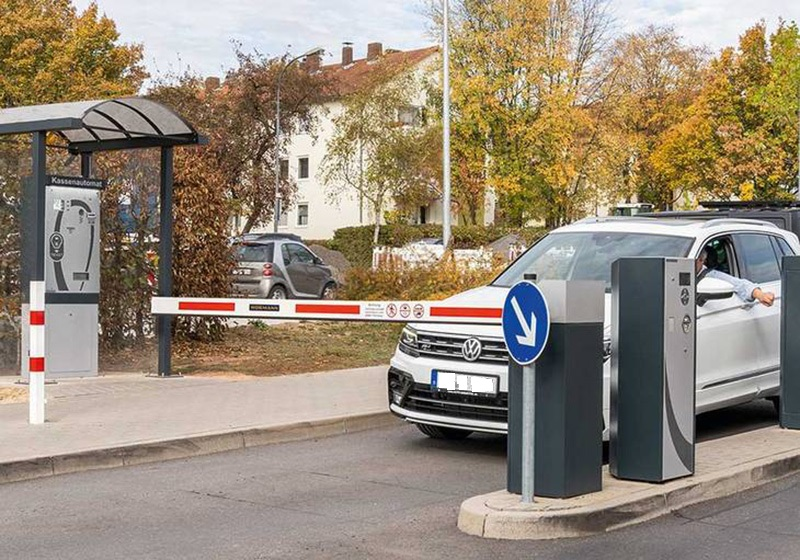
\includegraphics[width=0.5\textwidth]{imgs/sistema-control-acceso-barreras.jpg}
    \caption{Sistema tradicional de acceso por barreras \cite{integralia_sistema_2019}.}
    \label{fig:sistema-tradicional}
\end{figure}

Otro de los aspectos que destacan del uso actual del sistema de barreras en sistemas más manuales es la necesidad de
contar con  operarios trabajando en la barrera el tiempo que la barrera esté disponible, ya que en caso de no disponerlo
deberá quedar la barrera sin efecto, perdiendo por completo su utilidad.

\subsection{Sistemas Modernos}

Con el avance y el abaratamiento de los costos en la electrónica surgieron nuevos métodos que permitieron a los usuarios prescindir de la necesidad de un ticket o una tercera persona que les facilite el acceso, el método principal es el uso de controles remotos que al ser accionados, activan el mecanismo y abren el paso del vehículo.

Otro sistema que está ocupando gran parte del mercado en los últimos años es el que integra a la barrera un sistema de RFID, que mediante la colocación de un emisor RF en el vehículo, Fig.\ref{fig:sistema-moderno} o por el método de tarjetas o monedas de proximidad y un receptor en la barrera, al acercarse al ingreso se produce en el enlace que habilita o no al vehículo a ingresar. La gran desventaja de este sistema es tener que instalar el emisor RF en el vehículo o guardar la tarjeta de lectura.

Los problemas de este sistema son:

\begin{enumerate}
    \item Necesidad de instalar un emisor RFID.
    \item Distancia de actuación corta.
\end{enumerate}

\begin{figure}
    \centering
    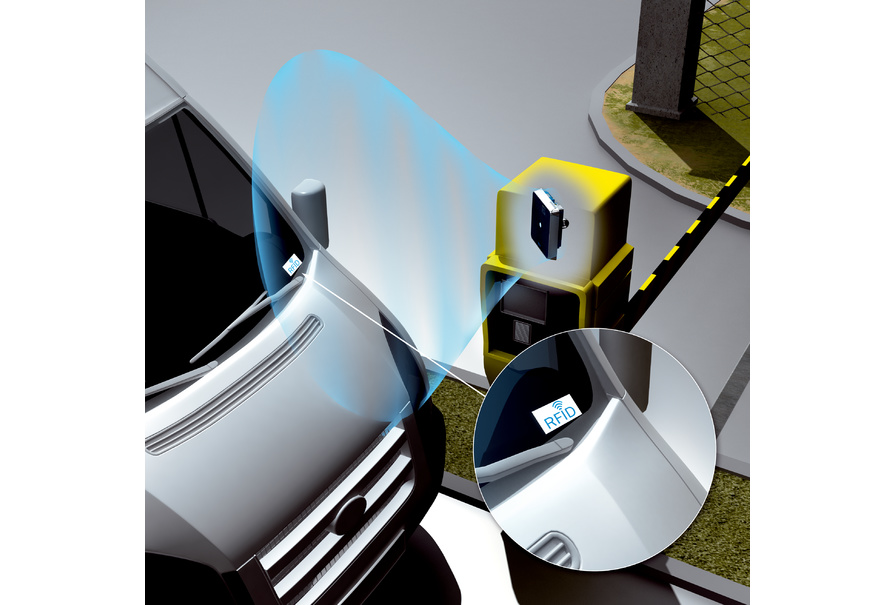
\includegraphics[width=0.8\textwidth]{imgs/sistema-control-acceso-barreras-rfid.jpg}
    \caption{Sistema moderno de acceso por barreras por sistema de RFID \cite{noauthor_acceso_nodate}.}
    \label{fig:sistema-moderno}
\end{figure}

\subsection{Requisitos de los sistemas SL}

Los métodos anteriormente nombrados son muy útiles en el día a día, pero cuentan con una serie de inconvenientes que pueden ser atenuados mediante el OCR, ya que se utiliza un distintivo único de los autos, como es el sistema de RFID, la distancia de actuación está dada por la distancia máxima de reconocimiento del algoritmo, y los sensores empleados.

Debido a la necesidad de realizar OCR, se requerirá una cámara. Con la finalidad de poder acoplar algún sistema de activación para la cámara se exigirá que la placa elegida soporte protocolos como I2C, SPI y UART. En cuanto a la comunicación, como se implementara junto con un servidor web existe la necesidad de conexión Ethernet o Wifi. Finalmente para facilitar futuras actualizaciones se requiere que la placa pueda correr un sistema operativo basado en GNU/Linux.

En resumen los requerimientos son:

\begin{enumerate}
    \item Implementación de una cámara.
    \item Soporte a protocolos I2C, SPI, UART.
    \item Conexión Ethernet o Wifi.
    \item Tiempo de acceso menor a 15 segundos.
    \item Sistema operativo basado en GNU/Linux.
\end{enumerate}


Entonces ¿Qué requisitos debe tener el sistema para cumplir lo planteado?, en primera instancia y como el eje del trabajo
es utilizar un algoritmo de OCR, el hardware debe permitir el uso de una cámara de al menos una resolución de 480p, debe
soportar protocolos de comunicación (i2c,spi o UART) para el acople de sensores auxiliares necesarios, permitir conexión
Ethernet/wifi, soporte para el uso de Python 3.

\section{Selección de placas}
Teniendo en cuenta los requisitos mínimos planteados en la sección anterior, se presentan varias opciones posibles,
placas de la empresa Raspberry Pi, embebidos de la serie STM32 e incluso placas de la marca Arduino en sus versiones más
potentes, por nombrar las más conocidas. Aquí es donde nos surge el primero de los inconvenientes para tomar la decisión,
cuál sería la mejor opción que cumpla tanto las necesidades que debemos cubrir, como también que sea accesible para poder realizar las pruebas y testeos correspondientes.
Por lo que empezamos a investigar con qué variedad de placas contábamos y podíamos llegar a conseguir de manera sencilla,
y se tomo la decisión de quedarnos con 2 placas que decidimos llamar modelo SL y SL mini.

\subsection{Modelo SL mini}
La placa de la barrera SL mini es una Raspberry Pi 3 B+ [referencia https://www.raspberrypi.com/products/raspberry-pi-3-model-b-plus/],Fig.\ref{fig:raspberry} la cual cuenta con un procesador
Broadcom BCM2837B0 y un Córtex A53 acompañado de 1 GB de RAM LPDDR2, lo cual es más que aceptable para correr un sistema operativo Raspberry Pi
OS(anteriormente conocido como Raspbian) basado en Debian(distribución de Linux), lo que era un requisito a cumplir desde
el comienzo del diseño del trabajo.

\begin{figure}
    \centering
    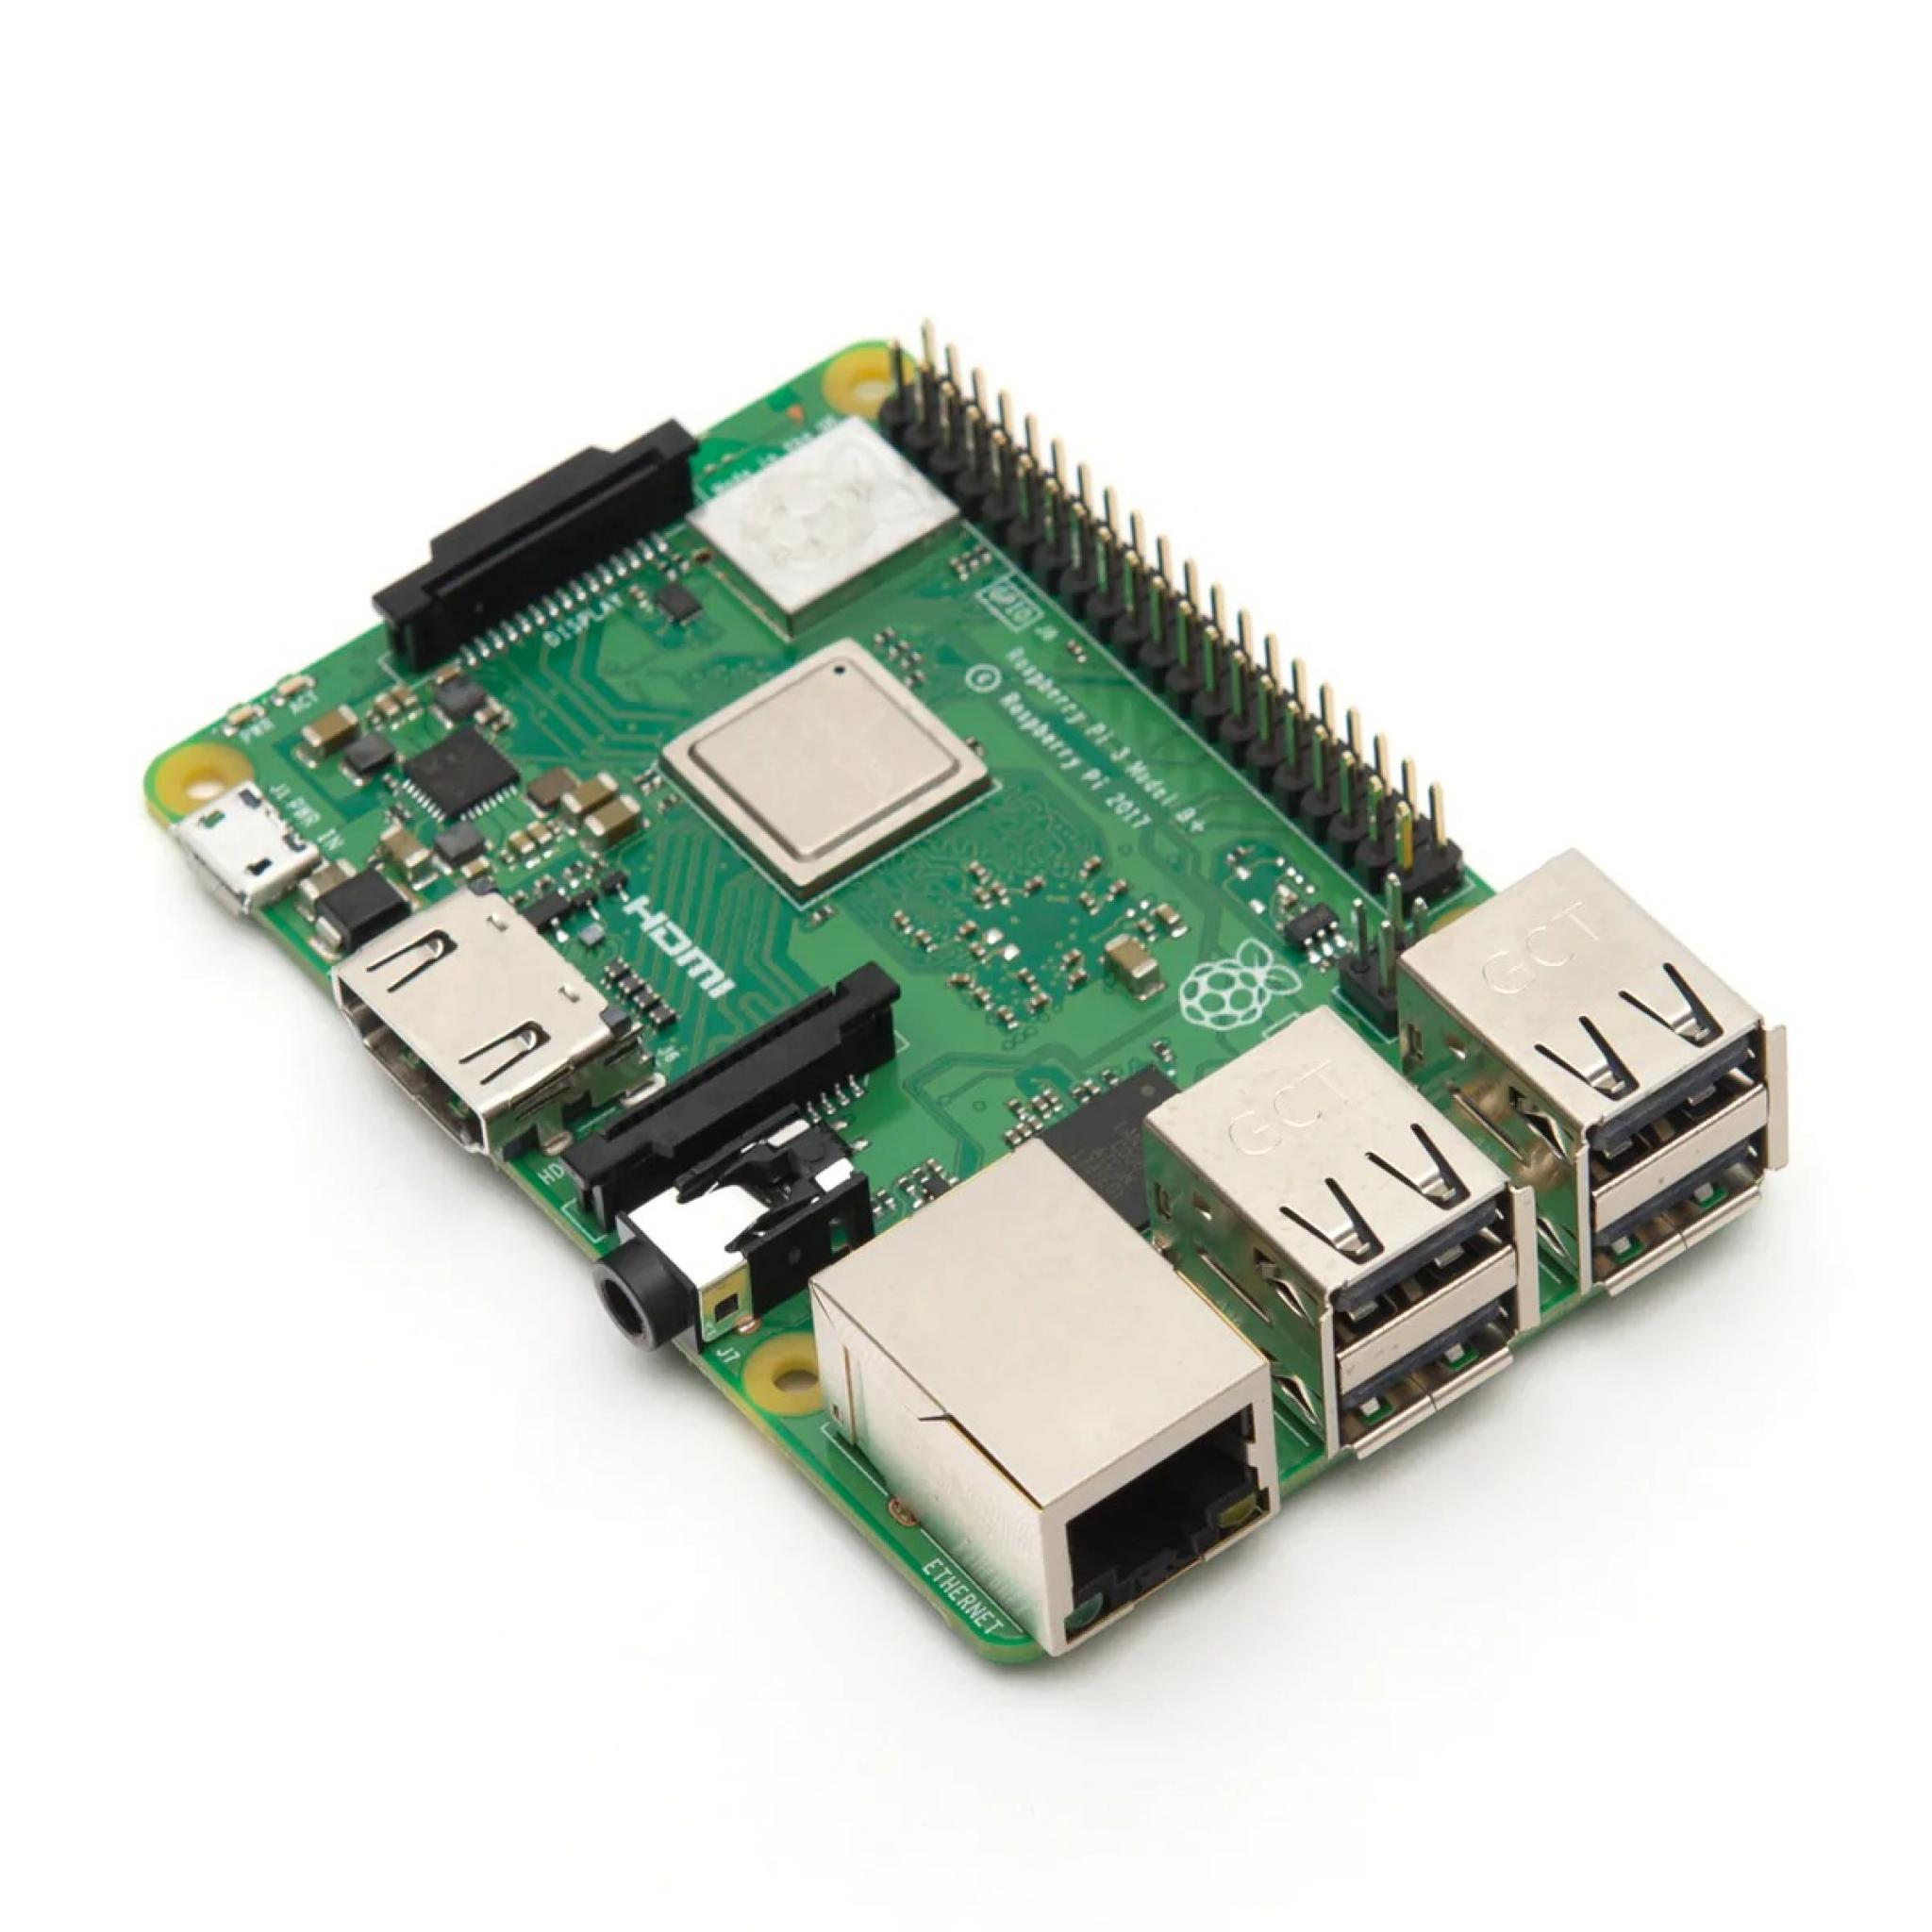
\includegraphics[width=0.8\textwidth]{imgs/Raspberry-pi3b+.jpg}
    \caption{Sistema embebido Raspberry Pi 3B+.}
    \label{fig:raspberry}
\end{figure}
Otro de los puntos importantes que destacan de la placa son los pines GPIO, pines de entrada/salida de propósito general
por sus siglas en inglés, lo que la hace sumamente sencilla a la hora de utilizarla junto a sensores comerciales.
La amplia conectividad integrada que posee fue un punto que la destacó sobre otras posibles placas de desarrollo, ya que
cuenta con puertos de conexión USB 2.0, puerto Gigabit Ethernet, conexión wifi 2,4 y 5,8 GHz y comunicación Bluetooth 4.2,
suple la necesidad de brindar conexión a internet de manera nativa sin necesidad de contar con periféricos extras que
puedan encarecer y obstaculizar el correcto funcionamiento del sistema.


La disponibilidad de la placa en el mercado, fue un punto importante que se consideró, ya que pensando en una futura
implementación del sistema a mediana o gran escala o la necesidad de cambio por rotura de la misma, podían dejar el
proyecto parado o inutilizado generando otros inconvenientes, además de que la placa es de nuestra propiedad, dándonos
completa disponibilidad para su uso.


Si bien las capacidades de la Raspberry son amplias, para este proyecto su poder de cómputo no fue suficiente para realizar por sí misma el procesamiento de la imagen en un tiempo menor a 15 segundos, ya que demora un aproximado de 1:30 minutos, tiempo que se consideró excesivo.

\subsection{Modelo SL}
La placa de la barrera SL es una Nvidia Jetson TX1[referencia https://developer.nvidia.com/embedded/jetson-tx1],Fig.\ref{fig:JTX1} la cual cuenta con un procesador Córtex A57, pero
cuenta con la característica de contar con núcleos de procesamiento de imagen, más específicamente posee 256 núcleos Nvidia Maxwell,
lo que la vuelve una opción excelente en lo que se refiere al trabajo con imágenes y videos, además su 4GB de RAM LPDDR4,
la hacen una opción mucho más potente en capacidad de cómputo que la Raspberry Pi 3 B+.


Para la realización del presente trabajo se contó con el kit de desarrollo provisto por la empresa Nvidia para el uso
del sistema embebido, en él se pueden encontrar todas las conexiones mencionadas en la barrera SL mini, lo que permite
el paso de los sensores de una placa a otra con suma facilidad.

\begin{figure}
    \centering
    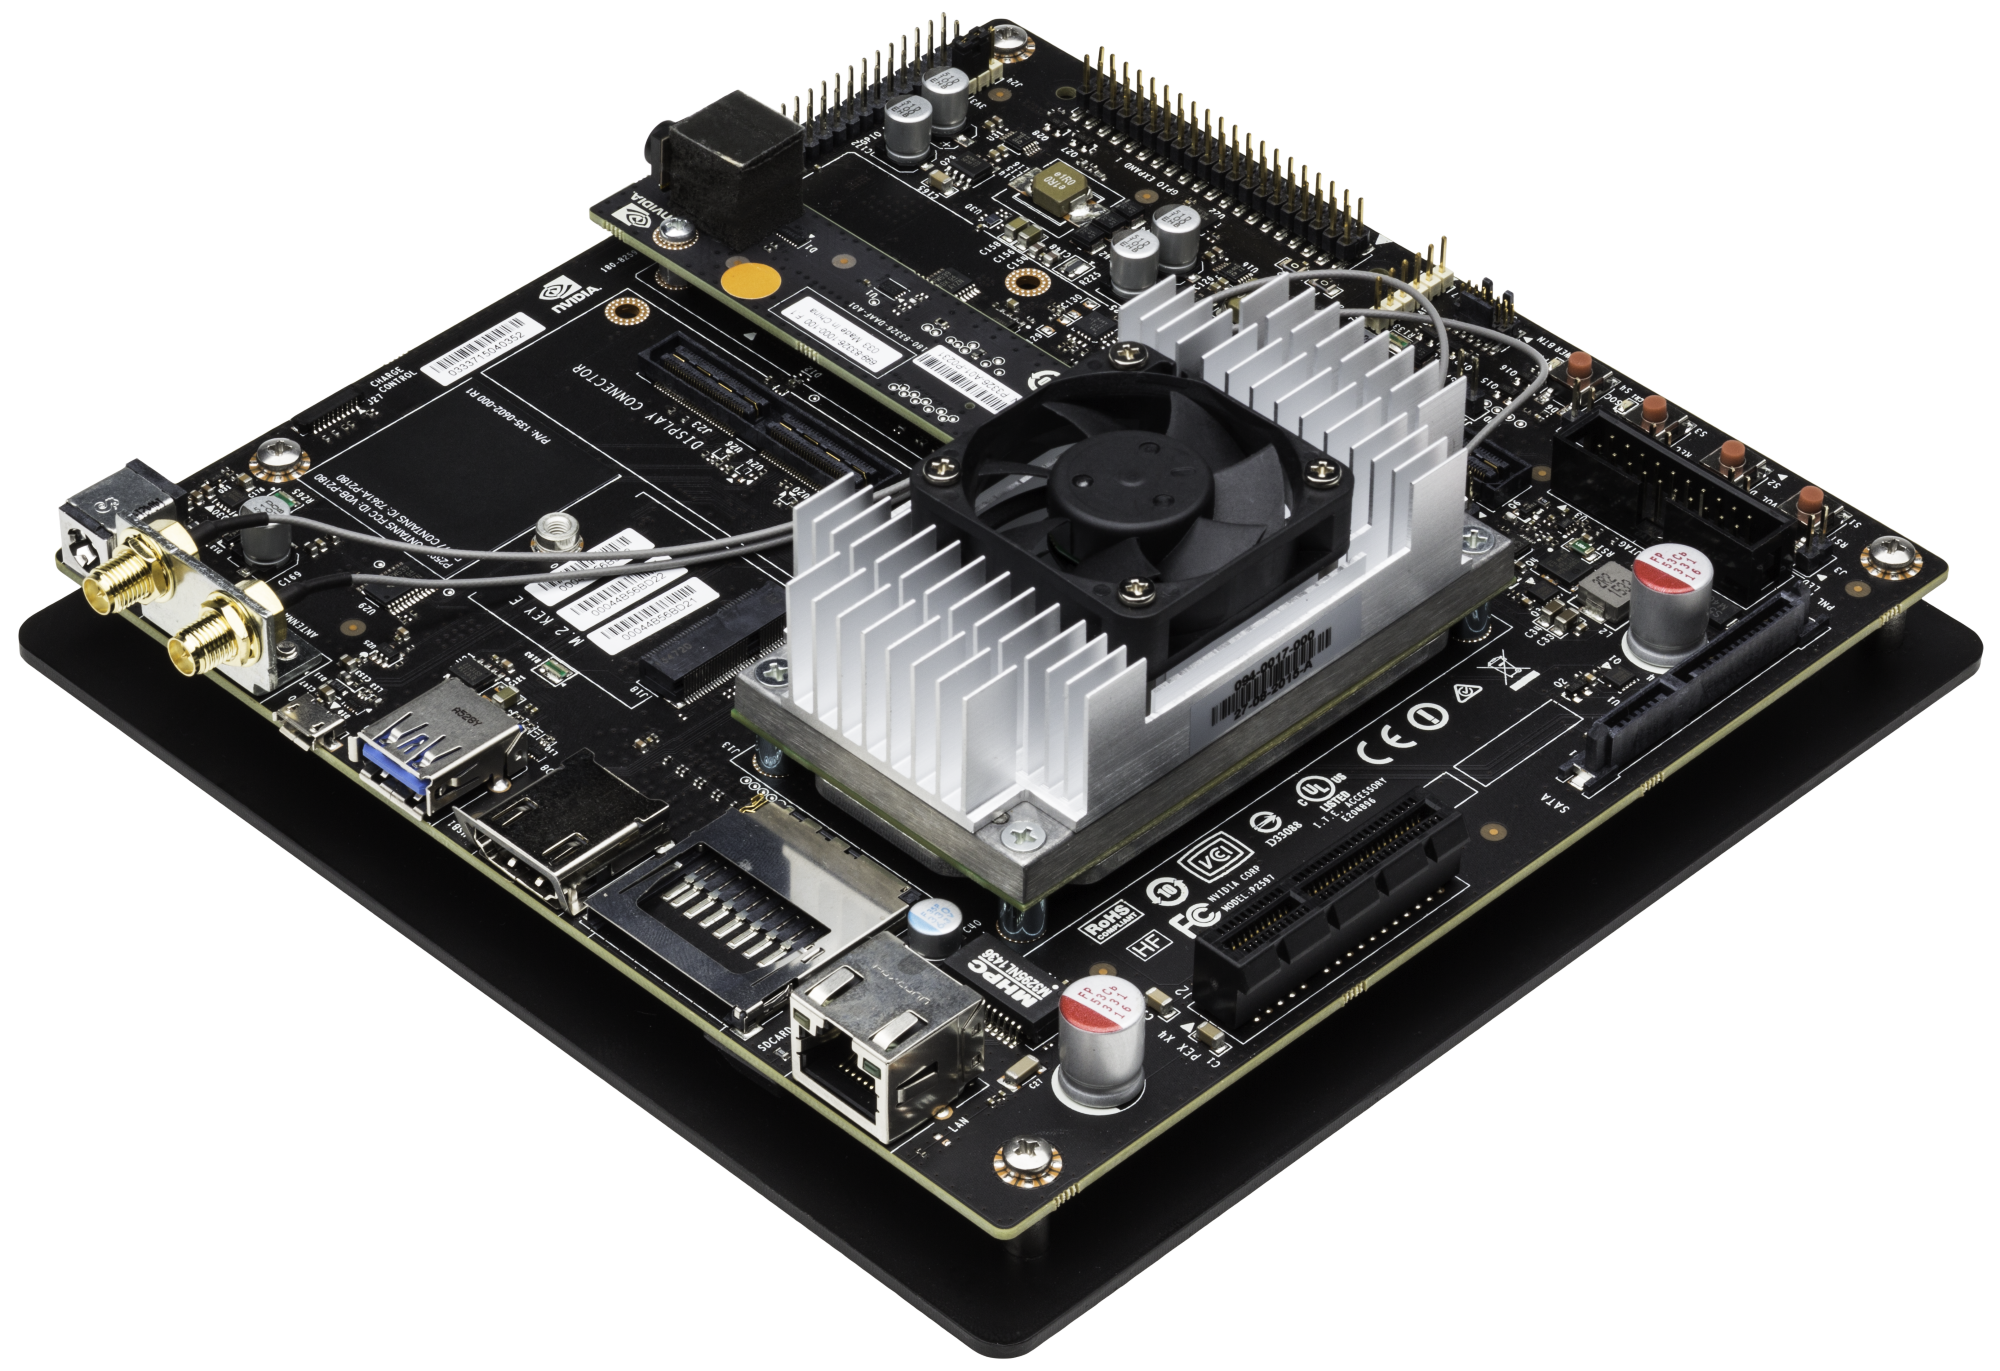
\includegraphics[width=0.8\textwidth]{imgs/JTX1-developerkit.png}
    \caption{Sistema embebido Nvidia Jetson TX1 developer kit.}
    \label{fig:JTX1}
\end{figure}


En contra parte con el modelo mini, la placa del modelo SL está pensada para el trabajo con redes neuronales y el manejo de imágenes, por lo que es posible integrar todo el sistema de reconocimiento de caracteres dentro del mismo algoritmo embebido en la placa, teniendo un tiempo de respuesta de aproximadamente unos 6 segundos, tiempo que se consideró aceptable.

\section{Evaluación y selección de sensores}

En este apartado se comentará la selección de la cámara y el proceso de selección del sistema de actuación, que como se adelantó en el capítulo 2 se decantó por un sensor de distancia.

\subsection{Selección de cámara}

Una cualidad importante para la selección del tipo de cámara fue la interfaz que esta utilice, lo que permite utilizar el mimo modelo en ambas versiones de placa. Si bien, tanto Raspberry como NVIDIA proveen de módulos de cámara, debido a que los conectores no eran los mismos se descartaron estas opciones. La decisión final terminó siendo una cámara web con interfaz USB, debido a que hoy en día son fáciles de conseguir y son relativamente económicas. Particularmente el modelo utilizado es el que se observa en Fig. \ref{fig:camara-usb}, el cual es un modelo genérico con una resolución de $1280x720$ y $0.9MP$, siendo estas características aceptables para la tarea requerida.

\begin{figure}
    \centering
    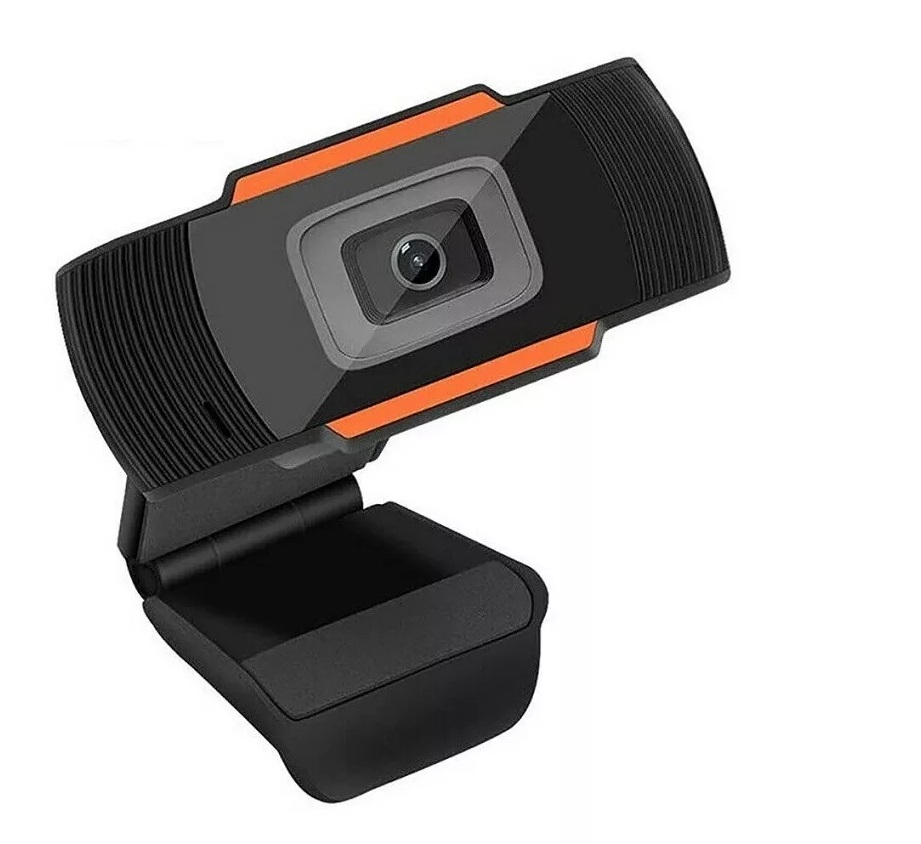
\includegraphics[width=0.5\textwidth]{imgs/camara-usb.jpg}
    \caption{Cámara utilizada para obtención de imágenes.}
    \label{fig:camara-usb}
    %https://www.mercadolibre.com.ar/camara-webcam-para-pc-microfono-usb-720p-hd-windows-10/p/MLA21775903#searchVariation=MLA21775903&position=2&search_layout=stack&type=product&tracking_id=8191aaa4-4b06-41e0-b681-ded2c4d4b641
\end{figure}

\subsection{Selección de activador}

Con la finalidad de minimizar las imágenes sin vehículos, se decidió colocar un sensor capaz de señalar que existe un objeto. A continuación se nombran las opciones analizadas:

\subsubsection*{Barrera infrarroja}

Este sistema cuenta con un receptor y un emisor, separados lo suficiente para que un vehículo pase entre ellos. La captura se da cuando el vehículo interrumpe el paso de luz entre el receptor y el emisor.

El sistema de barrera infrarroja cuenta con una serie de inconvenientes que dificultan su implementación como:

\begin{enumerate}
    \item Potencia mínima para activar el receptor.
    \item Potencia máxima que puede emitir el trasmisor.
    \item Ruido producido por la luz ambiente u otras fuentes lumínicas.
    \item Apantallamiento del receptor debido a partículas de suciedad.
\end{enumerate}

\subsubsection*{Placa de presión}

La placa de presión cuenta de una placa que acciona un interruptor cuando es presionada. Debido a que no fue posible armar un sistema de placa a presión, y tampoco se consiguió una opción económicamente viable, sumado a que las dimensiones pueden variar dependiendo el estacionamiento esta opción fue descartada.

\subsubsection*{Sensor de distancia}

Los sensores de distancia son muy versátiles y existen una amplia variedad en el mercado es por ello que fueron seleccionados para la implementación de los prototipos.
En particular para este trabajo se utilizó un sensor ultrasónico US-100.

Los sensores ultrasónicos funcionan emitiendo una onda ultrasónica por el transmisor y medir el tiempo que está tarda en llegar al receptor.

El US-100 el cual se puede apreciar en Fig. \ref{fig:sensor-US100}, posee un rango de medición de $2cm$ a $350cm$, compensado por temperatura, voltaje de alimentación entre $3V$-$5V$ y usando el protocolo de
comunicación UART.
Por lo que es fácilmente integrable en ambas placas por medio del puerto GPIO sin necesidad de utilizar hardware extra.
\begin{figure}
    \centering
    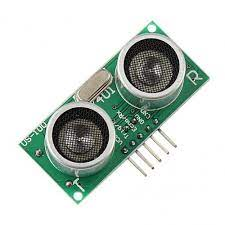
\includegraphics[width=0.5\textwidth]{imgs/us-100.jpg}
    \caption{Sensor US-100 usado en los prototipos.}
    \label{fig:sensor-US100}
\end{figure}

\section{Consumo energético}

El gasto energético es un punto que fue analizado, ya que, pensando en el uso racional de la energía, queríamos que nuestros prototipos no
presentaran un consumo excesivo, y que en un futuro si alguien lo deseaba sean alimentando por un panel solar junto con una batería.
Como la energía suministrada al conjunto cámara-sensor viene dada por las placas, solo se indicara el consumo requerido por las placas SL y SL mini.
\subsection{Consumo energético Modelo SL}

El requerimiento energético previsto por el fabricante para el kit de desarrollo de la Nvidia Jetson TX1 como se indica
en el cargador que viene dentro del kit es de $19V$ y $4.74A$, dando un máximo de $90W$, 9 veces mayor al del sistema SL mini.

\section{Diseño y ensamble}

Para la colocación del conjunto de prueba cámara-sensor, se diseñó e imprimió un contenedor en 3D,Fig. \ref{fig:contenedor-camara}
que sera soportado por un trípode o puede ser anclado a una pared o poste cercano a la zona de acceso.
\begin{figure}
    \centering
    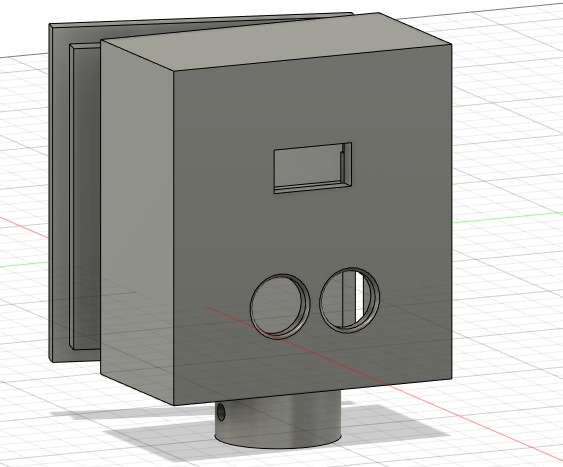
\includegraphics[width=0.5\textwidth]{imgs/contenedor-camara.png}
    \caption{Modelo 3D del contendor del paquete cámara-sensor.}
    \label{fig:contenedor-camara}
\end{figure}

Se optó por colocar el sensor de proximidad en la zona inferior, ya que el ideal es colocar el contenedor a una altura de unos $60cm$ aproximadamente, con lo que al tener el sensor en la zona baja se garantiza que la lectura que se tome sea de la trompa del automóvil y se obtenga un valor certero de la distancia. Este diseño deja a la cámara en la zona superior del contendor dando una imagen lo más completa de la trompa del vehículo, lo que permite que el sistema reconozca la patente de mejor manera, esto previene que la patente salga recortada permitiendo mejores resultados en la etapa de estimación. Se dispuso un orificio en la zona inferior de la caja con la finalidad de colocar un eje, que permita la orientación del dispositivo, dependiendo
el lugar donde se desee instalarlo, para la sujeción al eje se realizaron 2 pequeños orificios que permitan el paso de 2 tornillos que dejen fijo
el contenedor al eje.
\begin{figure}
    \centering
    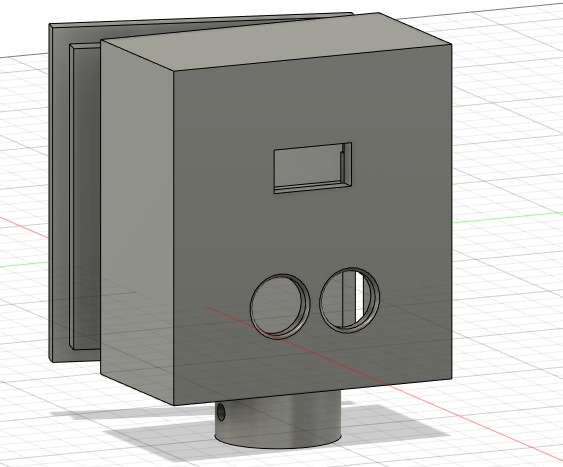
\includegraphics[width=0.5\textwidth]{imgs/contenedor-camara.png}
    \caption{sistema de sujeción del contenedor.}
    \label{fig:sujecion-contenedor}
\end{figure}

En la Fig. \ref{fig:contenedor-camara-real} se puede apreciar el contenedor ya con la cámara y el sensor instalados.

\begin{figure}
    \centering
    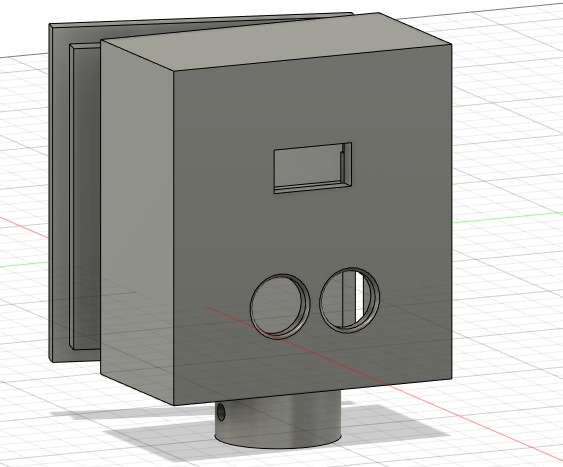
\includegraphics[width=0.5\textwidth]{imgs/contenedor-camara.png}
    \caption{Contendor del paquete cámara-sensor.}
    \label{fig:contenedor-camara-real}
\end{figure}

\section{Implementación de los drivers}

Para terminar el diseño de los sistemas SL y SL mini, se explicará el diseño de los drivers. Durante la etapa de diseño el eje fundamental fue crear piezas de códigos reutilizables y priorizando el diseño modular del sistema, algo que incluso ha sido una decisión general de diseño a lo largo de este trabajo. Es por ello que se implementaron una serie de módulos que permiten una actualización sencilla de los mismos, aíslan responsabilidades en diferentes partes y permiten un crecimiento del sistema más sencillo. La implementación se realizó en Python 3. A continuación se realizara una breve explicación de las librerias creadas.


\subsubsection*{Lectura de distancia}

Para la lectura de distancia se implementó una librería llamada \textit{us100}, la cual utiliza \textit{pyserial} \cite{noauthor_documentacion_nodate-1} para la comunicación por puerto serie. Esta librería posee una función la cual devuelve la distancia de un objetivo, pero con la finalidad de disminuir un objeto que se cruza o una mala medición se utiliza una lista anidada que posee las últimas 5 mediciones, y devuelve el promedio de las mismas.

\subsubsection*{Utilidades}

Se creó una librería llamada \textit{slutils} la cual tiene como responsabilidad la conexión con el servidor MQTT, el envío de registros de entrada/salida, así como administrar la configuración del sistema y la captura de imágenes.

Para la conexión con el servidor MQTT se utilizó \textit{paho-mqtt} \cite{craggs_documentacion_nodate}, escuchando el tópico \textit{$id/config$} donde el $id$ es un identificador único por cada placa.

En cuanto al envío de los registros este se realiza por POST mediante HTTP utilizando la librería \textit{requests} \cite{python_software_foundation_documentacion_nodate}.

La captura de imágenes se realizó mediante la librería de \textit{OpenCV}, la cual permite una fácil conexión con la cámara USB permitiendo tomar fotografías rápidamente.

\subsection{Diferencias entre SL y SL mini}

Como fue nombrado con anterioridad, la mayor diferencia entre ambos sistemas es que el sistema SL es capaz de procesar la imagen de manera local. Esto implica que una conversión de los modelos de Tensorflow \cite{google_tensorflow_nodate} utilizados para la CNN-OCR a una versión capaz de correr en ARM, por lo que se compilaron los modelos a Tensorflow Lite, utilizando las herramientas que Tensorflow provee para estos casos. Por otro lado, se requiere compilar la YoloV4 para arquitectura ARM, este paso se realizó utilizando el compilador de CMake.



\chapter{Diseño e implementación del servidor}

En este capítulo se explicará el diseño y la implementación del server. En la Fig. \ref{fig:server-final} se observa la versión final del servicio, mostrando la interacción entre los Clientes, los sistemas SL y el Server.

\begin{figure}[h]
    \centering
    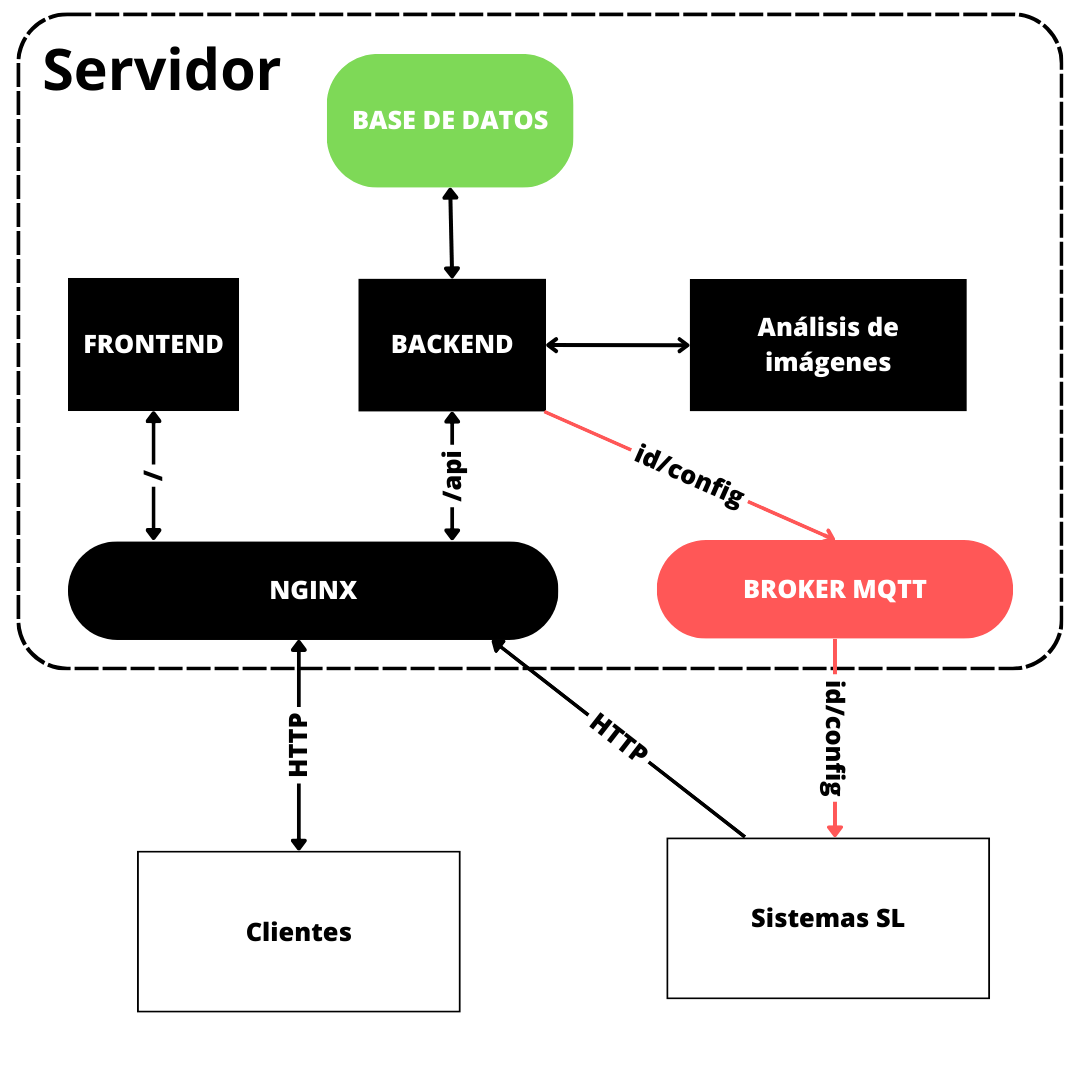
\includegraphics[width=.6\textwidth]{imgs/server-esquema.png}
    \caption{Esquema final del servidor.}
    \label{fig:server-final}
\end{figure}

\section{Actualidad del desarrollo web}

En la web existen dos grandes mundos: el Frontend es la parte de la web con la que interactúan los usuarios o clientes. El Backend que es la parte que se conecta con la base de datos y ejecuta las validaciones necesarias para leer o escribir información. En general, el frontend y el backend suelen ser 2 proyectos separados y pueden ser construidos en diferentes lenguajes. Los lenguajes más utilizados son: JavaScript (JS), Python, Ruby, entre otros \cite{presta_10_2021}.

En la actualidad el formato más utilizado para trasmitir información entre el Backend y el Frontend se utiliza el formato JSON de sus siglas en inglés JavaScript Object Notation o traducido como notación de objetos de JavaScript. En la Fig. \ref{fig:ejemplo-json} se observa un ejemplo de JSON. Este tipo de notación se caracteriza por almacenar los datos en forma clave-valor, permitiendo que el acceso a la información sea rápido y sencillo.

\begin{figure}
    \centering
    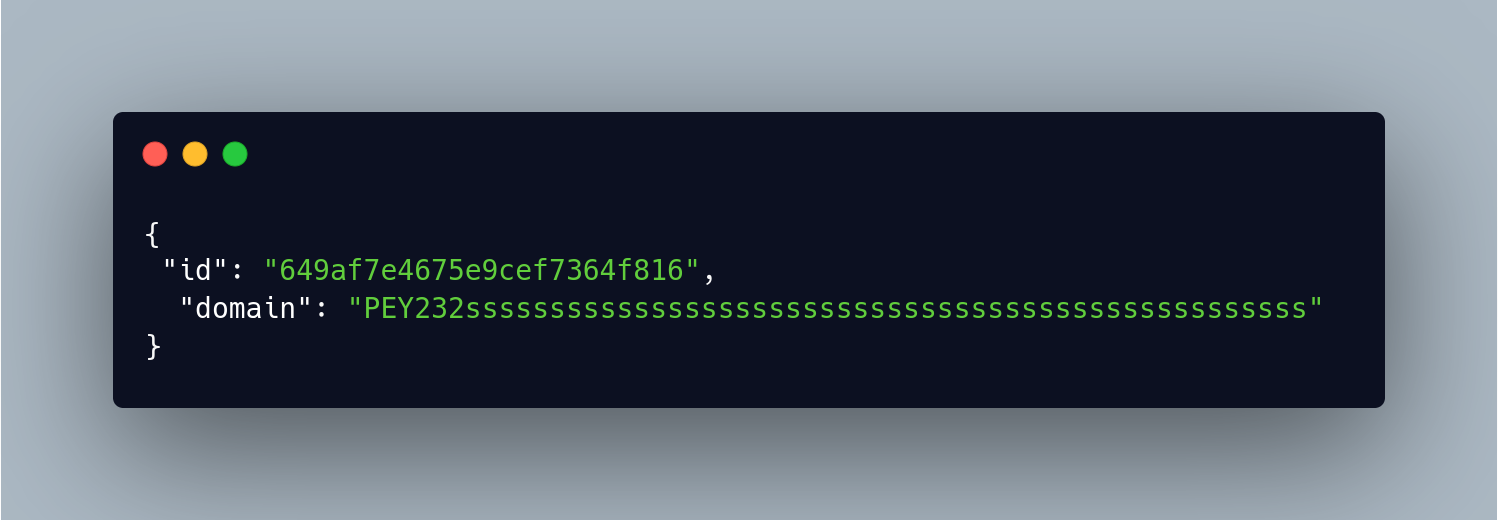
\includegraphics[width=.5\textwidth]{imgs/json-example.png}
    \caption{Ejemplificación de un JSON.}
    \label{fig:ejemplo-json}
\end{figure}

Hoy en día la web se ha transformado en la base de cualquier organización, hace años las organizaciones solían usar aplicaciones de escritorio, pero en la actualidad las aplicaciones web han dominado el mercado.

\section{Docker}

Docker es una tecnología open source desarrollada por Docker Inc, la cual permite correr aplicaciones de forma aislada en contenedores.

\subsection{¿Qué es un contenedor?}

Un contenedor funciona casi como una máquina virtual, pero sin entorno gráfico y compartiendo el Kernel \cite{keepcoding_que_2022} con el sistema que lo hospeda, lo que hace que los contenedores sean más livianos y mucho más rápidos que una máquina virtual, ya que estas últimas emulan todo el sistema e incluyen un puente entren el kernel del sistema padre y el sistema emulado. Cada contenedor suele especializado para cumplir una determinada tarea, en general se los denomina servicios.

\subsection{Docker Compose}

Docker es una tecnología muy utilizada, pero por si sola puede ejecutar un único contenedor a la vez, es por ello que existen herramientas para la administración de múltiples contenedores en simultáneo. La más conocida, y muy utilizada en el mundo del desarrollo, es Kubernetes. Debido a que el sistema no es lo suficientemente grande y no se cuenta con múltiples servidores para alojar los servicios, la implementación se realizó mediante Docker Compose \cite{docker_inc_docker_2023}, el cual cumple un rol muy similar a Kubernetes, pero sin tanta complejidad extra que trae la opción de administrar múltiples servidores.
\begin{figure}
    \centering
    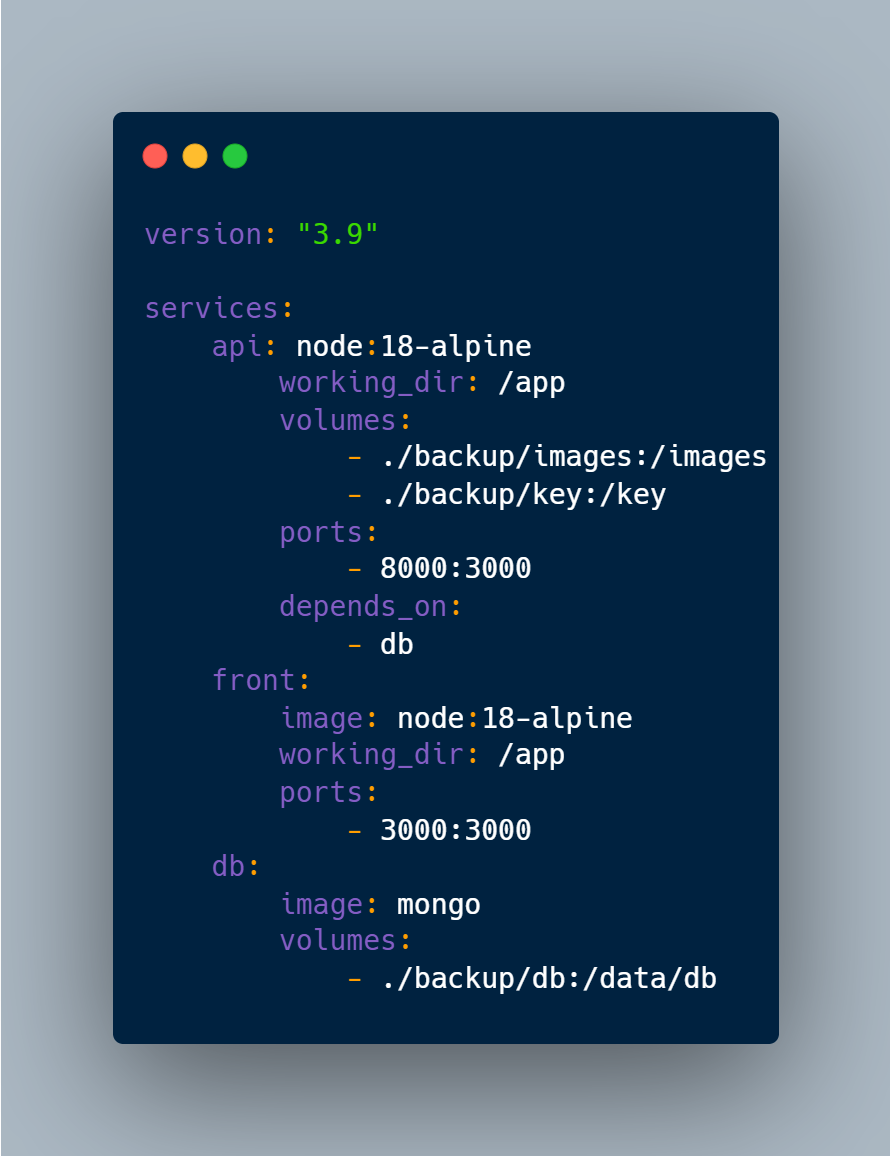
\includegraphics[width=.5\textwidth]{imgs/docker-compose.png}
    \caption{Ejemplificación de una archivo \textit{docker-compose.yml}}
    \label{fig:docker-compose-yml}
\end{figure}

El proceso de configuración de Docker Compose se hace creando un archivo de extensión YAML como el de la Fig. \ref{fig:docker-compose-yml}. Se puede observar que existen 2 apartados principales.

\subsubsection*{version}

Este atributo le indica a Docker Compose la versión del archivo de configuración que se está utilizando, en general, esta versión impacta directamente en qué atributos se pueden utilizar en el resto del archivo de configuración.

\subsubsection*{services}

Dentro del apartado de \textit{services} o por su traducción servicios se definen los servicios que se necesitaran, en este ejemplo se muestran 3 contenedores \textit{api}, \textit{front}, \textit{db}.

A su vez dentro de cada uno se define el atributo \textit{image} el cual indica que imagen se utilizará. Dicha imagen puede ser privada o  se puede utilizar una imagen pública de Docker Hub el cual es un repositorio de imágenes de Docker.
Las imágenes son en esencia un sistema operativo configurado para algunos entornos, por ejemplo la imagen \textit{node:18-alpine} posee un sistema Alpine, que ya viene instalado con NodeJS en su versión 18, imagen muy utilizada para correr aplicaciones escritas en JS.

Otro campo que se destaca es el \textit{working\_dir} o directorio de trabajo y es donde se almacenará el código de la aplicación. Es importante destacar que esta ruta se toma desde el contenedor, y no tiene por qué ser una ruta válida desde el sistema Host.

El atributo \textit{volumes} es un array que vincula una carpeta del sistema Host con una carpeta del contenedor, permitiendo acceder a la información del contenedor.
Esto es muy utilizado para realizar backup desde el sistema Host.

Por último \textit{ports} es un array que vincula los puertos del sistema anfitrión a los puertos del contenedor, lo que es sumamente útil cuando se desea escuchar un puerto específico para manejar peticiones HTTP, por ejemplo.

\subsubsection*{intranet}

Docker Compose genera una red interna para interconectar los contenedores, lo que permite que el servicio \textit{api} pueda acceder a la base de datos del servicio \textit{db} mediante la ruta \textit{mongodb://db:27017/sl}. La mayor ventaja de esta red es que hace inaccesible la base de datos para usuario que no estén dentro de la red de Docker, disminuyendo la vulnerabilidad del sistema.


\section{Servicios}

Una vez que fue descripto cómo se hará la implementación y su arquitectura, se procederá a entender cómo fue creada la aplicación web en su totalidad, describiendo cada parte del sistema.

\subsection{Base de datos}

La base de datos elegida fue Mongo DB, debido a que es una de las bases de datos más utilizada. Mongo es una base de datos basada en documentos, por lo tanto no posee vínculos fuertes entre los diferentes esquemas.
Los datos se almacenan en BSON (binary JSON), el cual hace más fácil la transferencia de datos. Por otro lado, permite escalar de manera horizontal de forma más sencilla, ya que se suelen usar identificadores únicos y no incrementales, como es frecuente en bases de datos del tipo SQL.

El esquema de base de datos [figura de la base de datos].

\subsection{Broker MQTT}

Debido a que Mosquitto es el broker MQTT más utilizado, el cual utiliza la versión 5.0 del protocolo. El único tópico implementado tiene la forma de ``\textit{id}/config" donde \textit{id} es un identificador único de la barrera, esto permite de que existan tantos tópicos como barreras, y solo pueden escuchar los cambios de configuración de ellas, lo que permite ahorrar procesamiento de datos en la barrera.

\subsection{Backend}

El Backend está implementado en NestJS \cite{noauthor_documentacion_nodate}. Su principal función es la de administrar la información porque se conecta con la base de datos para realizar las tareas de lectura y escritura de documentos.

Con la idea de generar la mayor documentación posible de este servicio se utilizó una librería llamada Swagger la cual, junto a NestJS, genera documentación automática de las rutas HTTP. Esto facilita la tarea de crear una nueva aplicación así como la de incluir una nueva persona al proyecto. En la Fig. \ref{fig:swagger-example} se observa como se ve la documentación generada por Swagger.

\begin{figure}
    \centering
    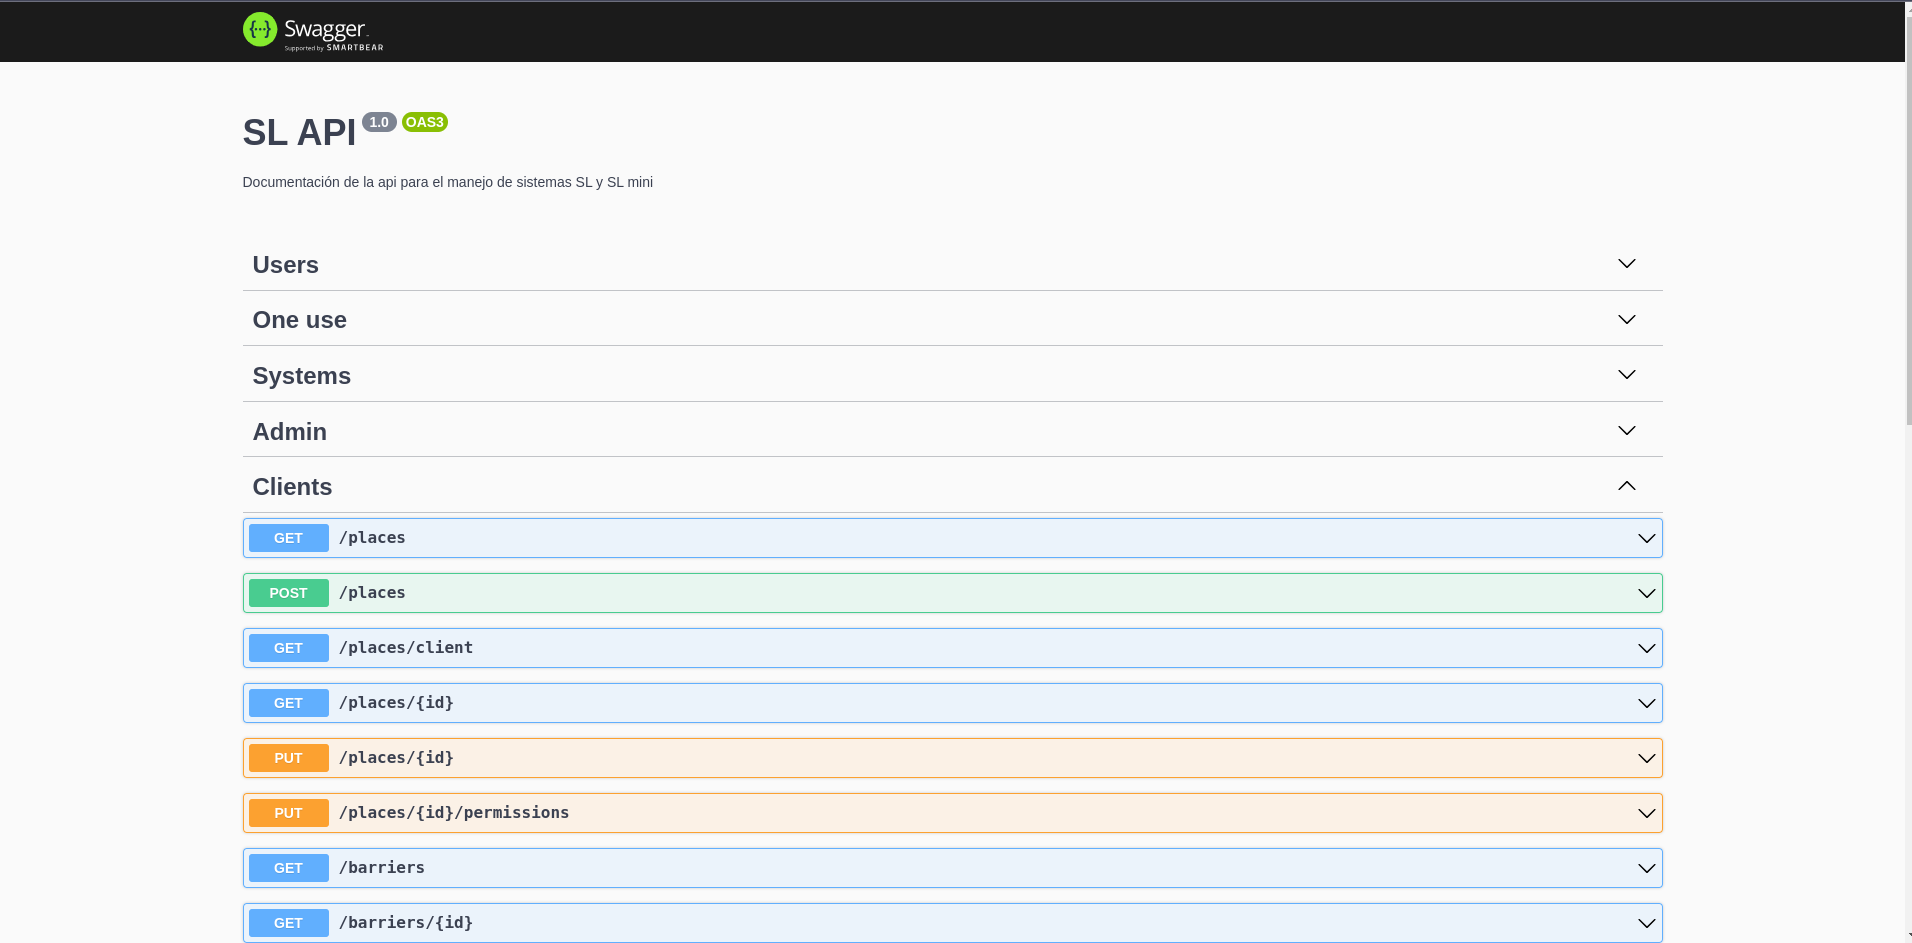
\includegraphics[width=\textwidth]{imgs/server/swagger.png}
    \caption{Documentación generada por Swagger.}
    \label{fig:swagger-example}
\end{figure}

Debido a la necesidad de autenticación de usuarios, y de los sistemas SL se implementó PassportJS que permite la creación de sistemas de validación de forma más sencilla. Los métodos de autenticación implementados fueron:

\begin{enumerate}
    \item Usuario y contraseña: Utilizado para los usuarios que entran/registran desde la web.
    \item ApiKey de terceros: Una forma de validar si la aplicación que pide datos está autorizada o no.
    \item ApiKey para barreras: Permite validar si la información del registro de entrada/salida está siendo enviada por una barrera autorizada. Además permite saber qué barrera es la que envía los datos, diminuyendo el tamaño de la petición.
    \item Json Web Token o JWT: Se utiliza una vez que el usuario entra a la app, y es un hash generado por el servidor.
\end{enumerate}

\subsubsection*{JWT}

JSON Web Token o simplemente JWT es un estándar qué está dentro del documento RFC 7519. Su función principal es poder propagar información entre dos partes de forma segura. En la práctica los JWT son muy fáciles de desencriptar por lo que se desaconseja incluir información sensible del usuario en el mismo.

\subsection{Análisis de imágenes}

Este servicio fue implementado con Flask el cual permite crear aplicaciones Backend en Python de forma fácil y rápida. La función de este servicio es obtener la patente de la fotografía tomada por los sistemas SL mini, es por ello que solo tiene una ruta e internamente ejecuta el algoritmo visto en el capítulo 3.

\subsection{Frontend}

El Frontend fue construido en ReactJS, que es una de las librerías de JavaScript más utilizadas en la industria. La idea principal de este servicio es brindar un centro de control de las barreras, además de permitir la visualización de registros y datos. Además permite a los administradores crear barreras nuevas y visualizar sus parámetros.

\subsubsection*{Páginas para los usuarios}

Los usuarios puede registrarse y entrar a la plataforma como se ve en la Fig. \ref{fig:login}. Luego de ingresar pueden visualizar sus estacionamientos (Fig. \ref{fig:home}).

Es posible configurar diversos parámetros del estacionamiento, como el nombre, ubicación y precio por hora (Fig. \ref{fig:update-place}).
Para agregar versatilidad al sistema y permitir su uso para diferentes tareas se implementó un sistema de bloqueo de patentes (Fig. \ref{fig:in-type}), que permite bloquear todas las patentes salvo las que se encuentren en la lista o bloquear solo las que se encuentren en la lista. Adicionalmente pueden visualizar las barreras por barrio (Fig. \ref{fig:barrier-details}) y desde esta vista pueden configurar los parámetros de las mismas en tiempo real (Fig. \ref{fig:update-barrier}).

Para la visualización y control de datos se crearon dos rutas.
El Dashboard permite ver información resumida: horas estacionadas y cantidad de vehículos estacionados, separados por estacionamiento, filtrar los datos según fecha de inicio y fin, además permite agrupar los registros día, mes o año (Fig. \ref{fig:dashboard}).
Por otro lado existe una vista de los registros crudos, dando información particular de cada registro (Fig. \ref{fig:registers})


\begin{figure}
    \centering
    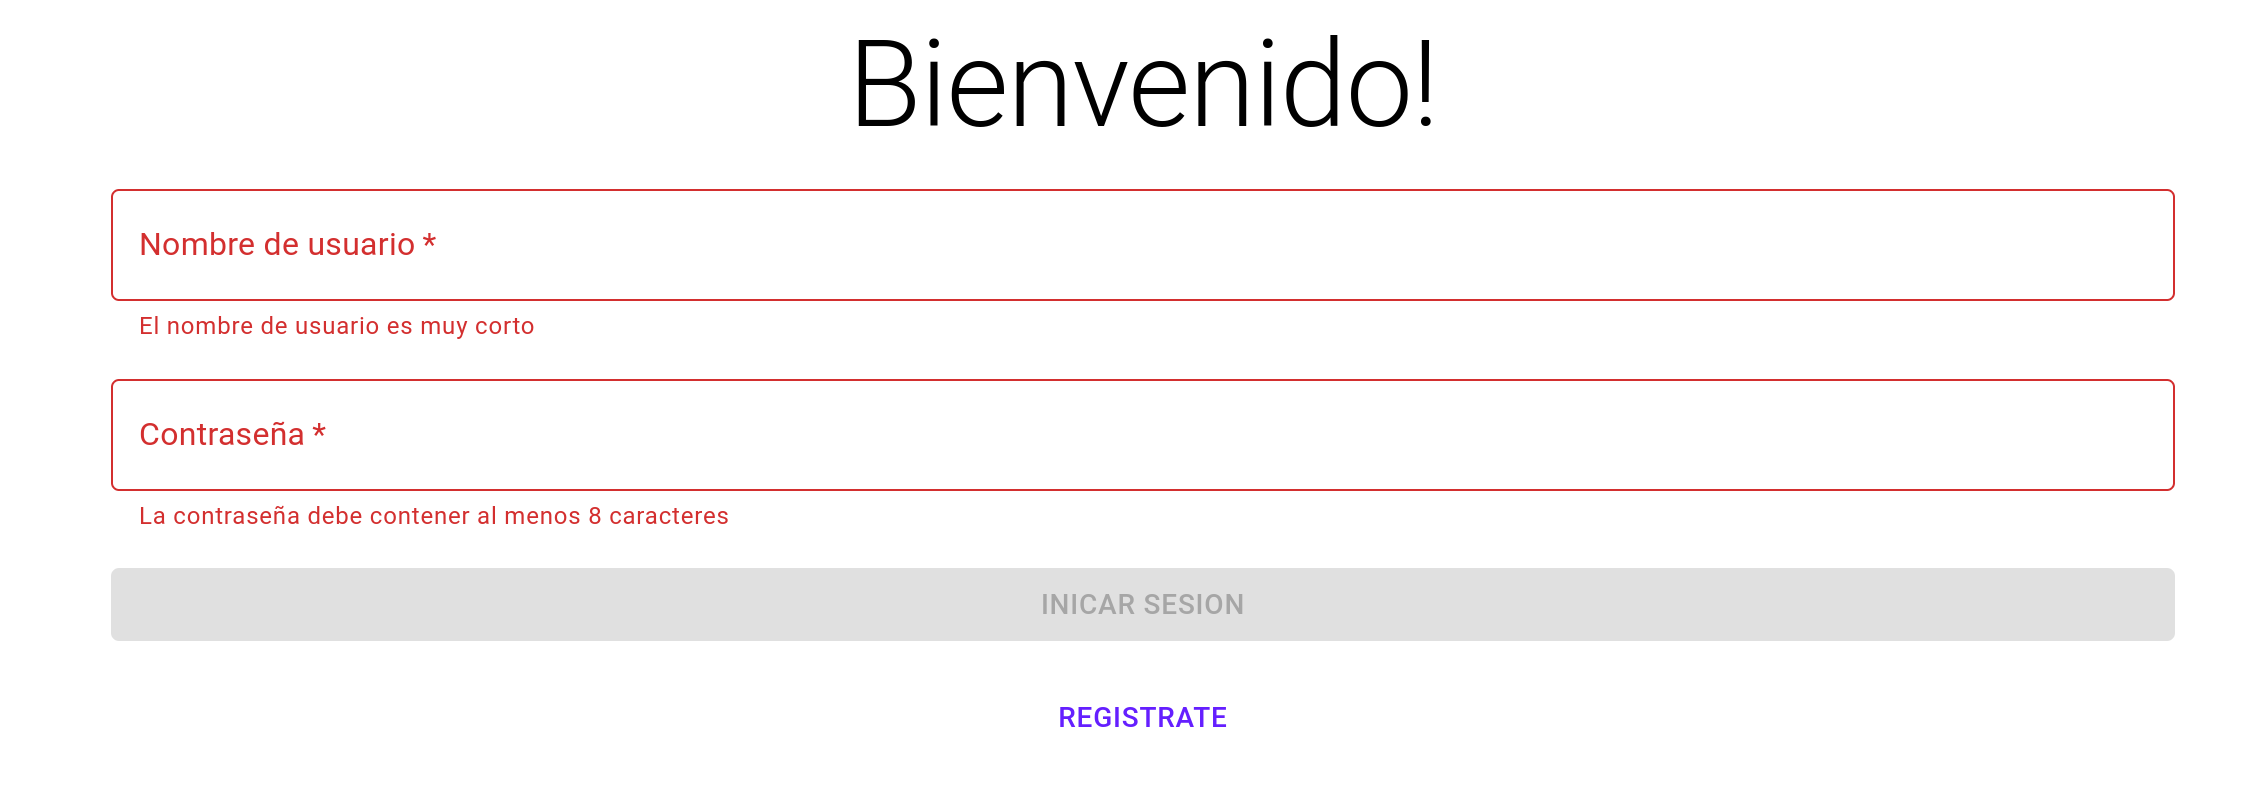
\includegraphics[width=\textwidth]{imgs/server/login.png}
    \caption{Inicio de sesión.}
    \label{fig:login}
\end{figure}

\begin{figure}
    \centering
    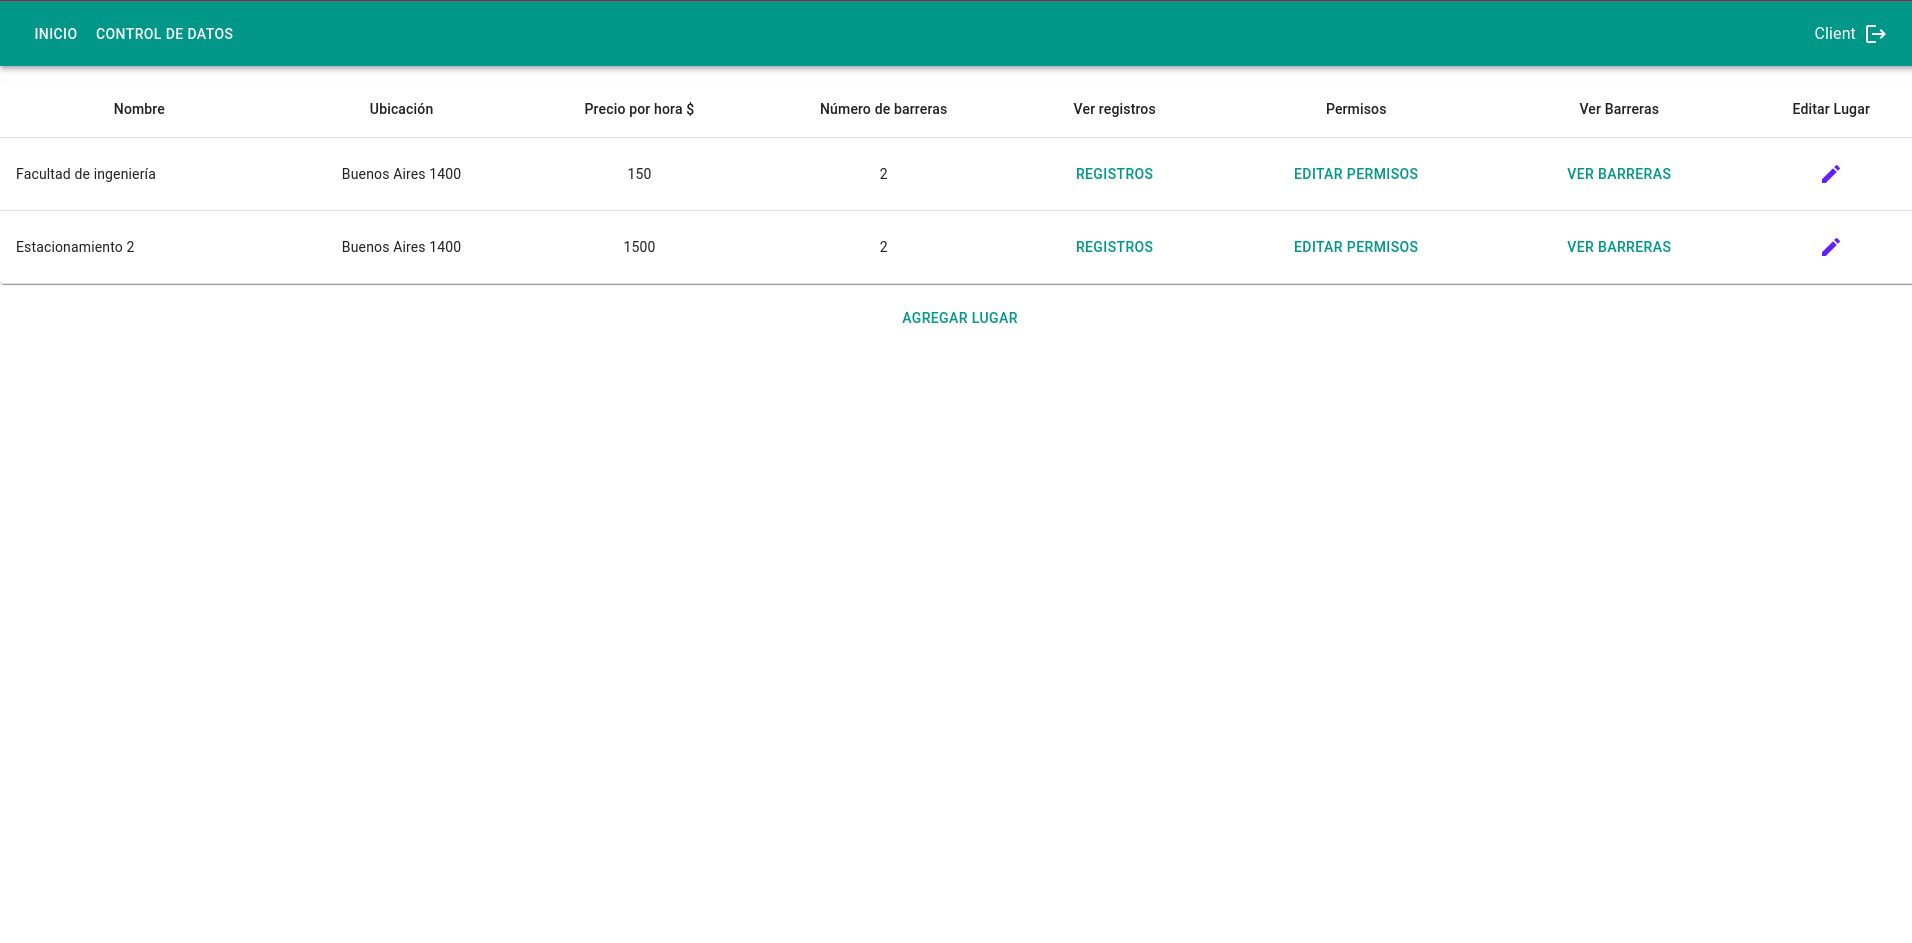
\includegraphics[width=\textwidth]{imgs/server/places.png}
    \caption{Estacionamientos del cliente.}
    \label{fig:home}
\end{figure}

\begin{figure}
    \centering
    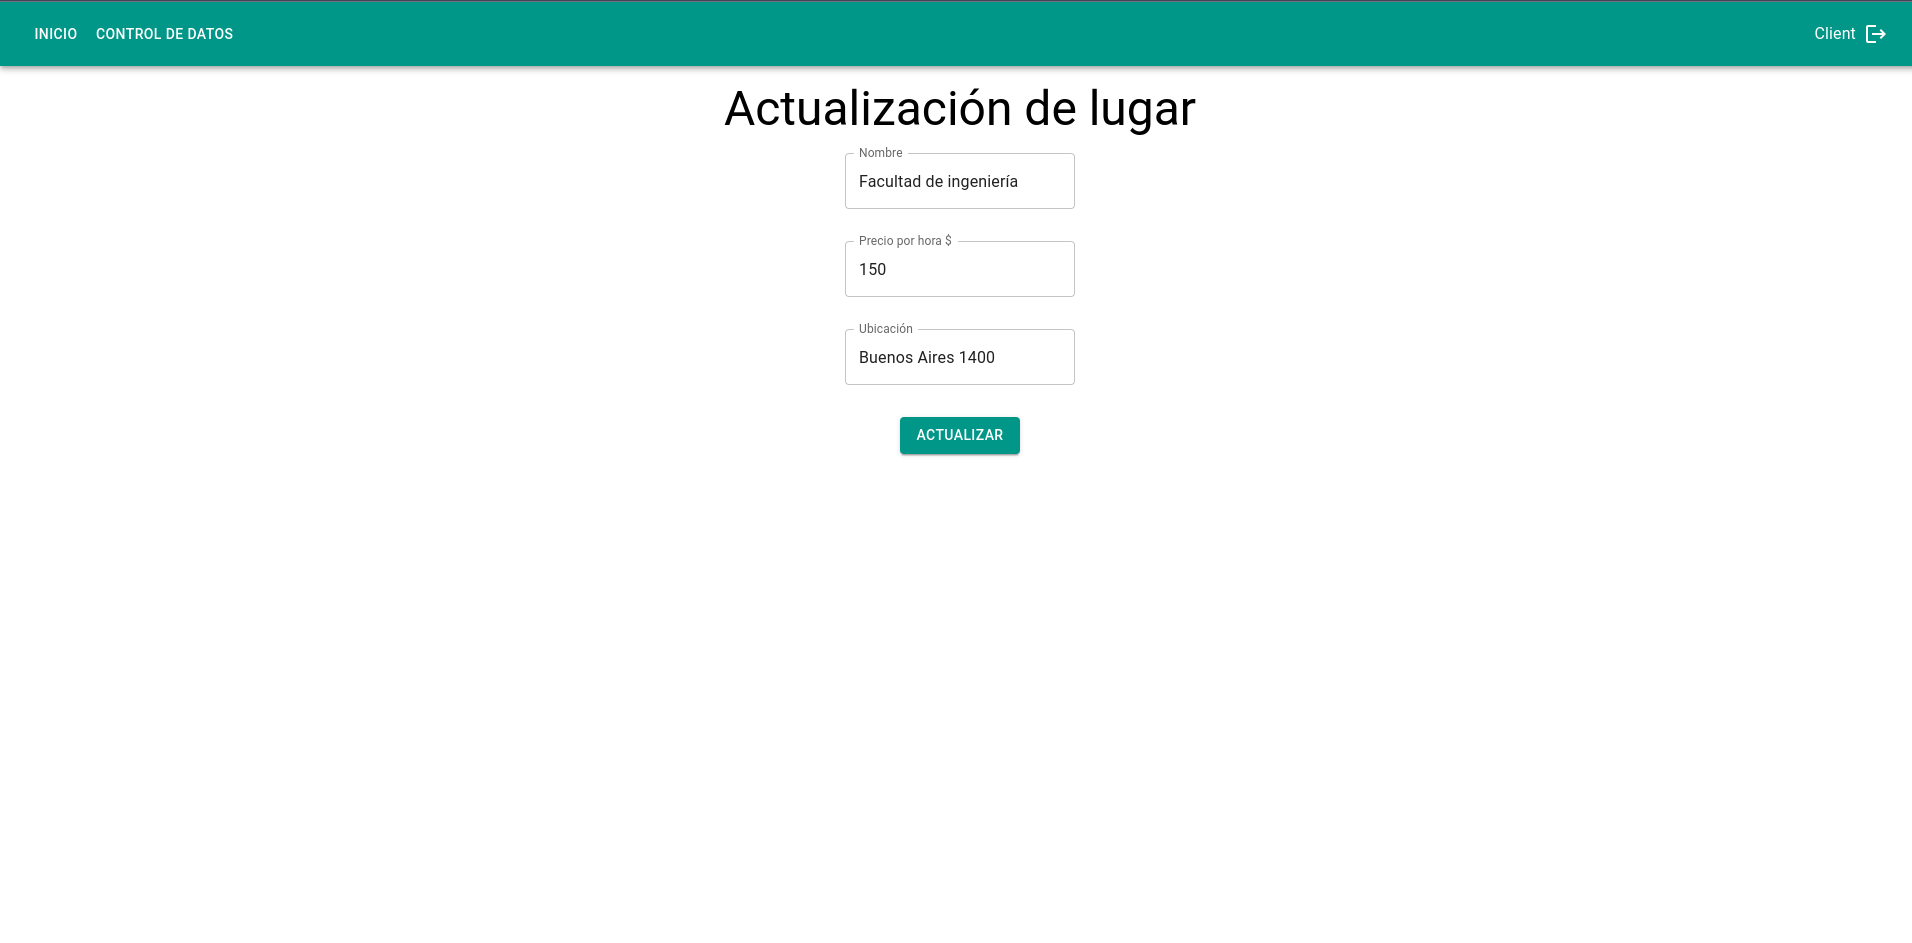
\includegraphics[width=\textwidth]{imgs/server/update-place.png}
    \caption{Formulario para actualizar un estacionamiento.}
    \label{fig:update-place}
\end{figure}


\begin{figure}
    \centering
    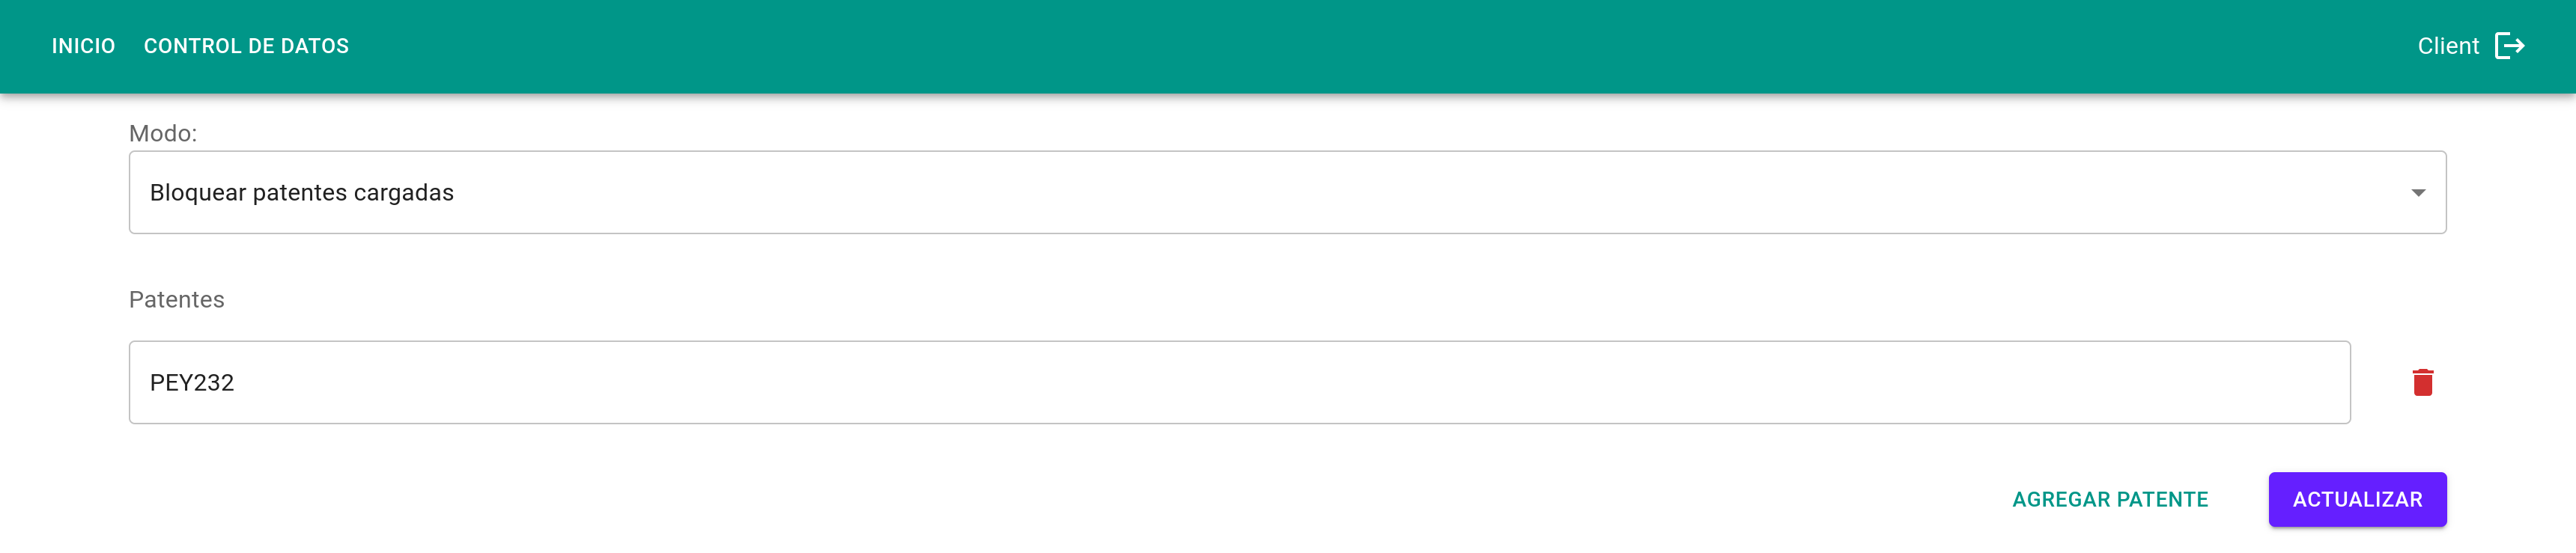
\includegraphics[width=\textwidth]{imgs/server/in-type.png}
    \caption{Vista de permisos.}
    \label{fig:in-type}
\end{figure}
\begin{figure}
    \centering
    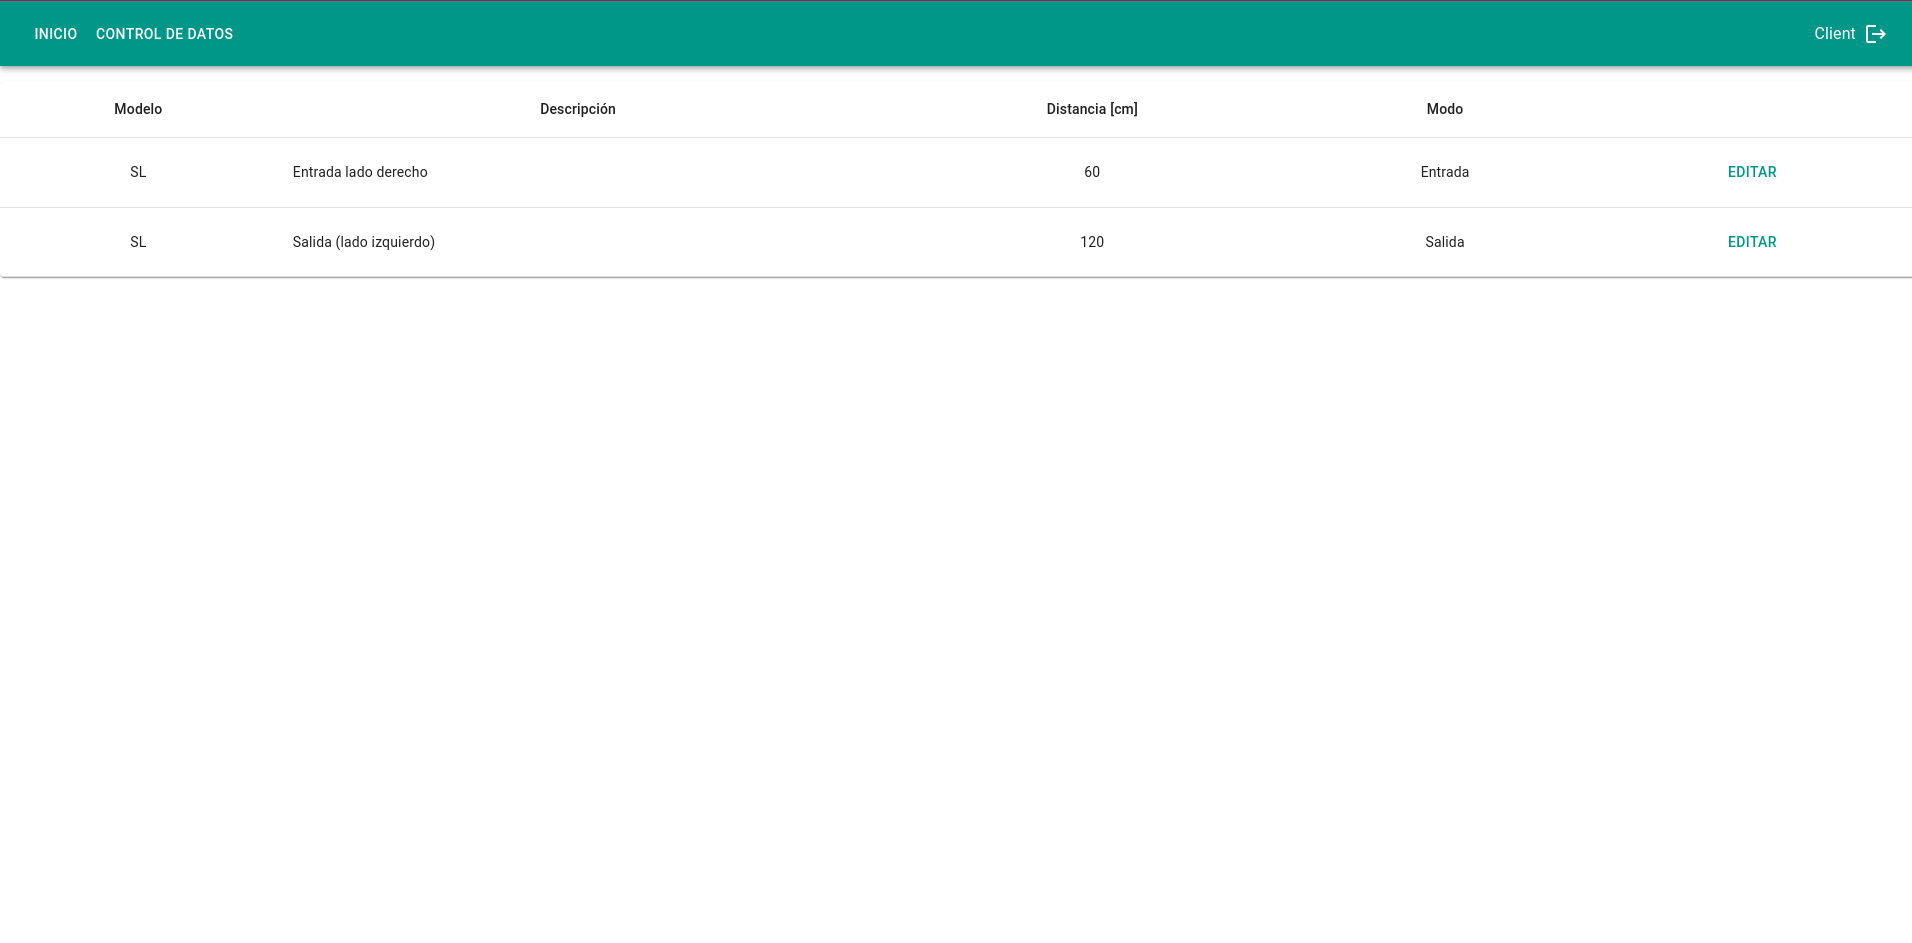
\includegraphics[width=\textwidth]{imgs/server/client-barriers-details.png}
    \caption{Vista de los detalles.}
    \label{fig:barrier-details}
\end{figure}

\begin{figure}
    \centering
    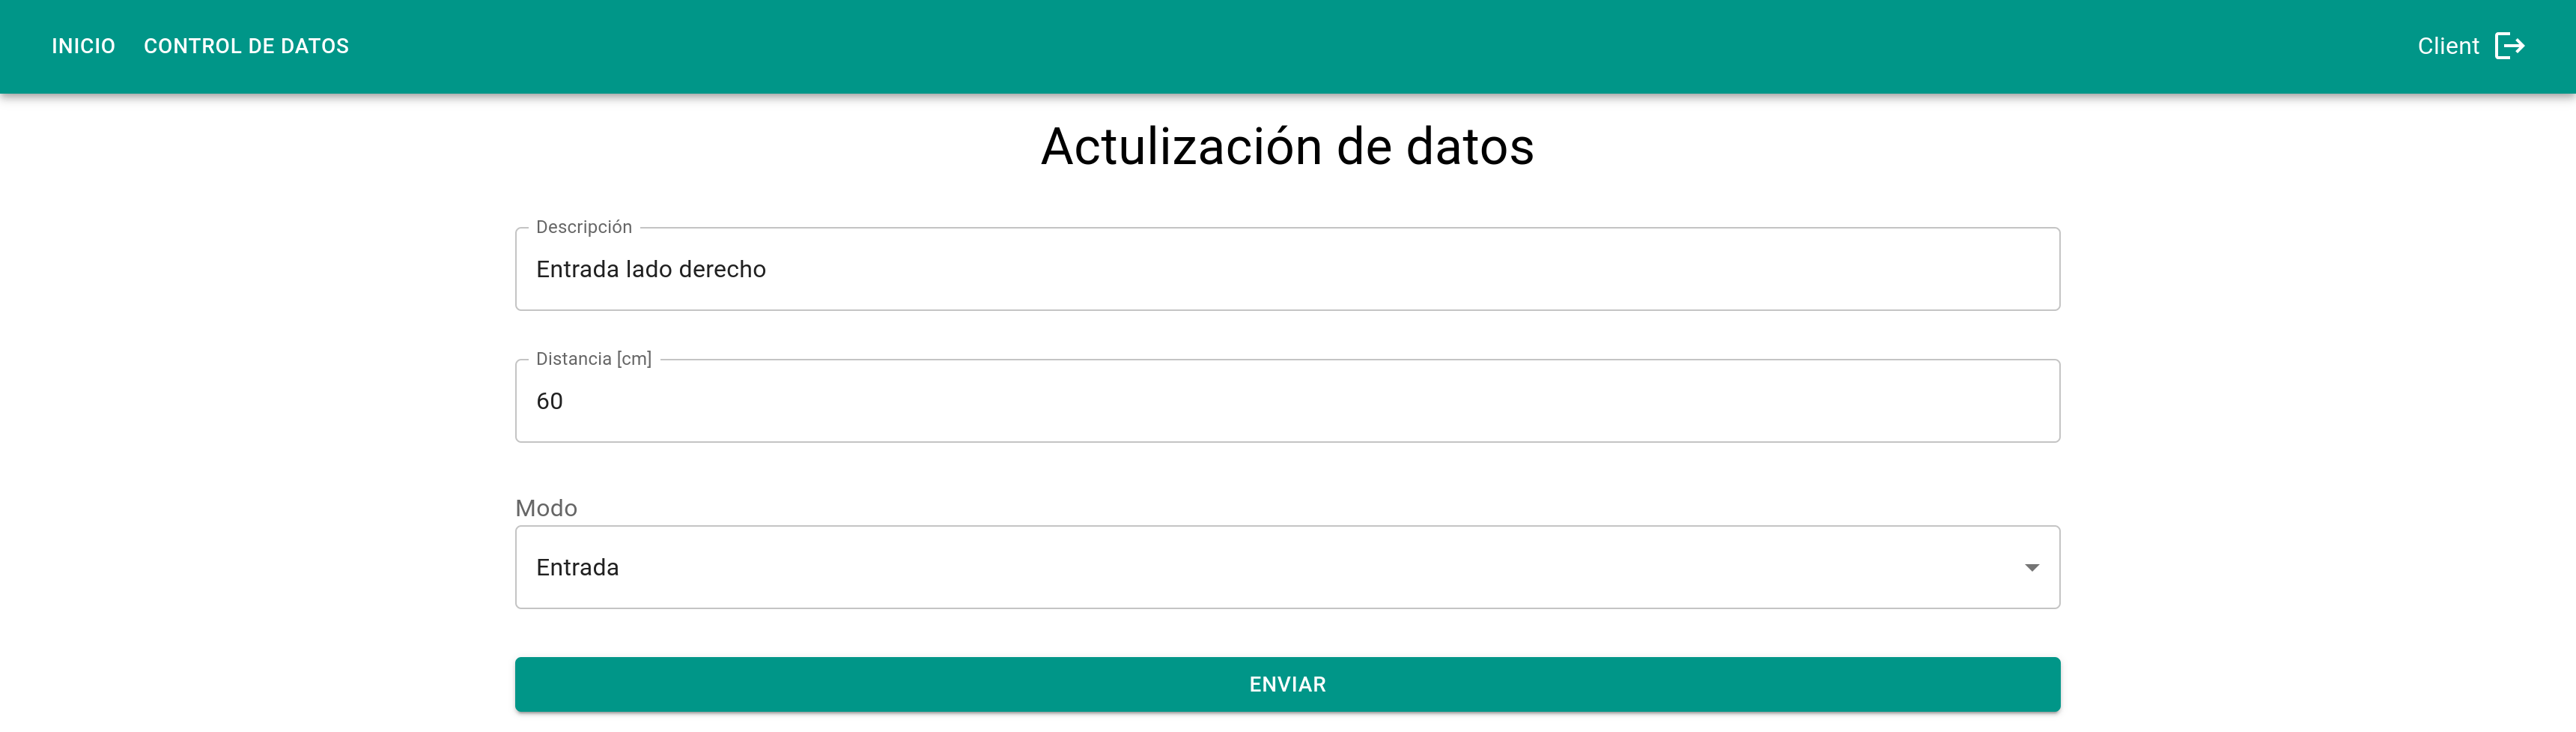
\includegraphics[width=\textwidth]{imgs/server/barrier-update-data.png}
    \caption{Formulario para actualizar los datos de la barrera.}
    \label{fig:update-barrier}
\end{figure}

\begin{figure}
    \centering
    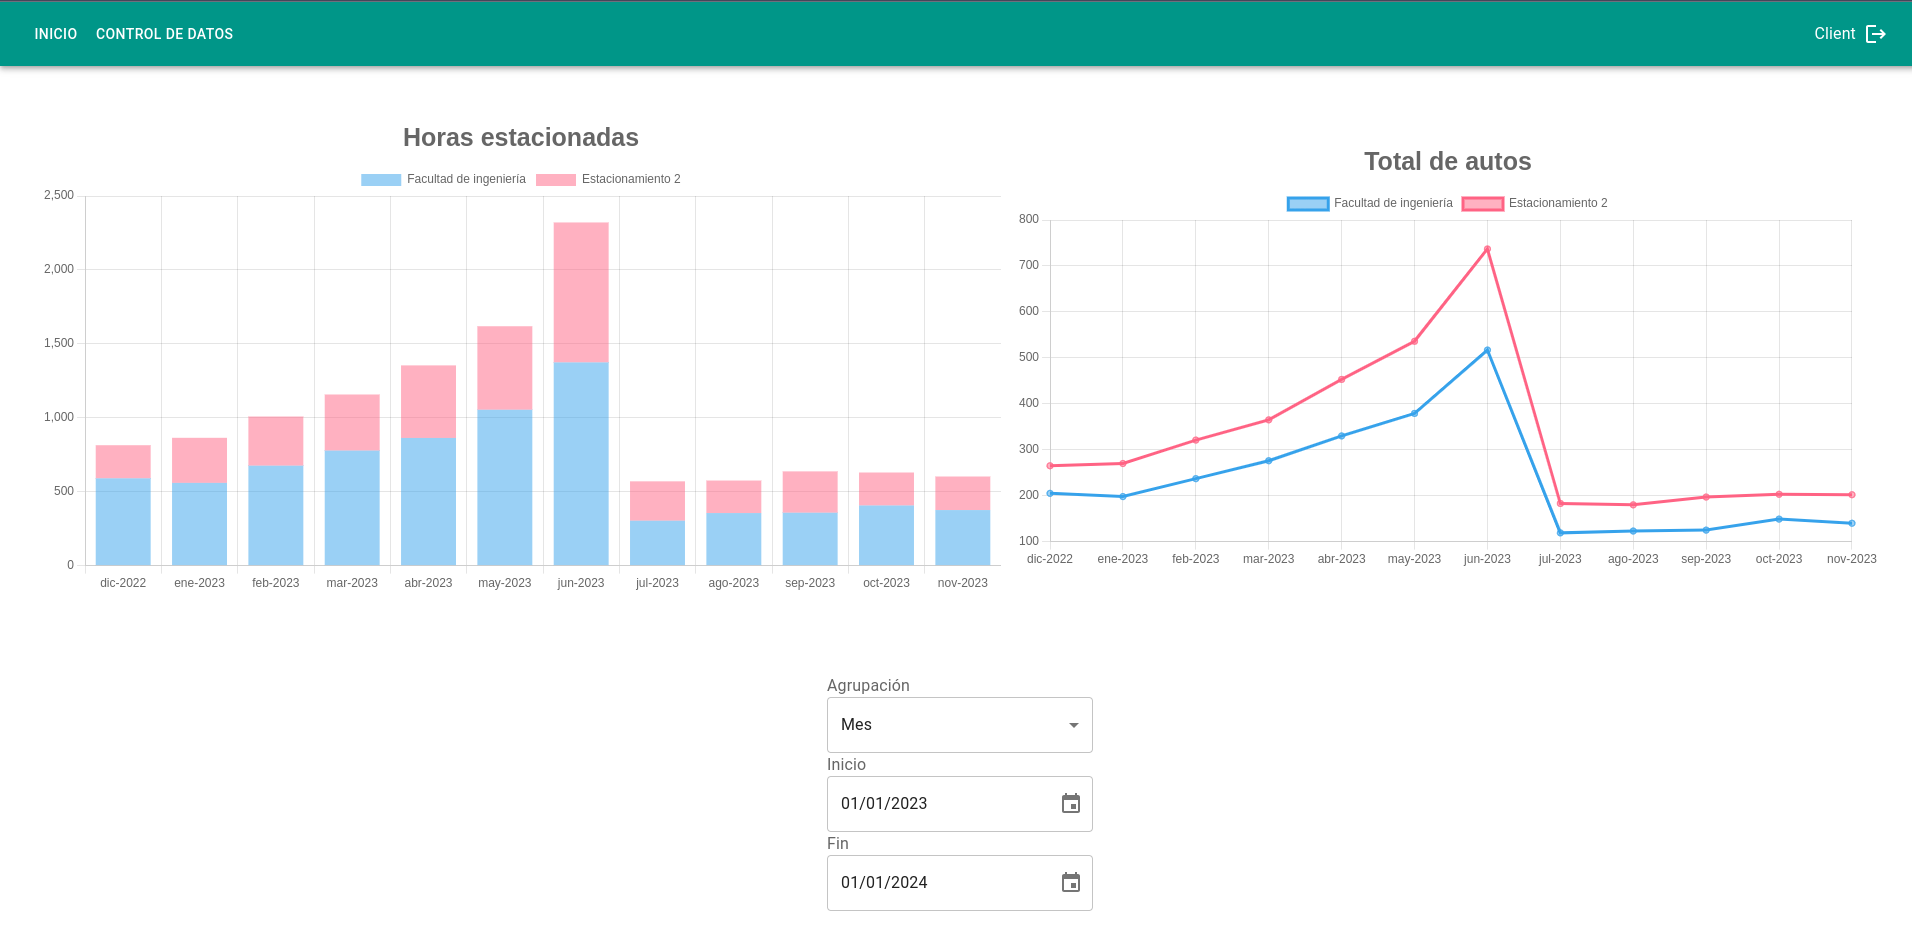
\includegraphics[width=\textwidth]{imgs/server/resume.png}
    \caption{Visualización de datos para un cliente con 2 estacionamientos.}
    \label{fig:dashboard}
\end{figure}

\begin{figure}
    \centering
    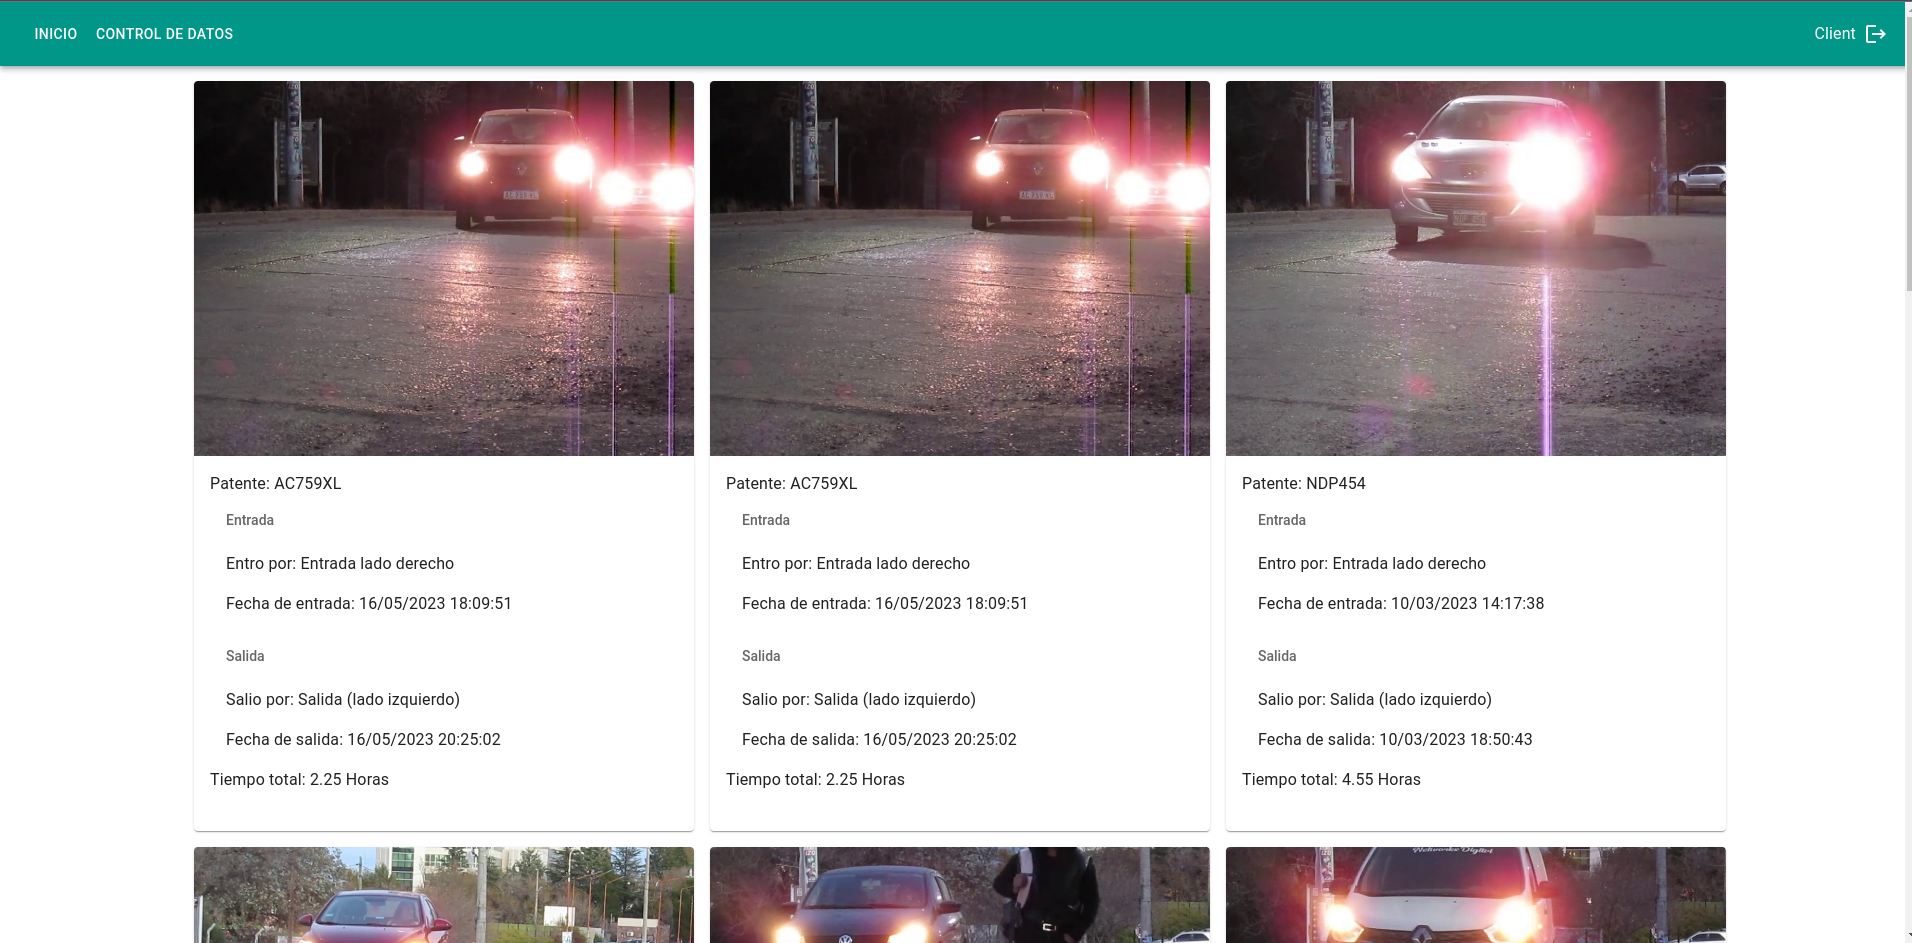
\includegraphics[width=\textwidth]{imgs/server/registers.png}
    \caption{Vista de registros.}
    \label{fig:registers}
\end{figure}



\subsubsection*{Páginas para los administradores}

Los administradores poseen una página para visualizar las barreras según cliente y lugar (Fig. \ref{fig:admin-details}). Por último, poseen una página para agregar barreras (Fig. \ref{fig:add-barrier}).

\begin{figure}
    \centering
    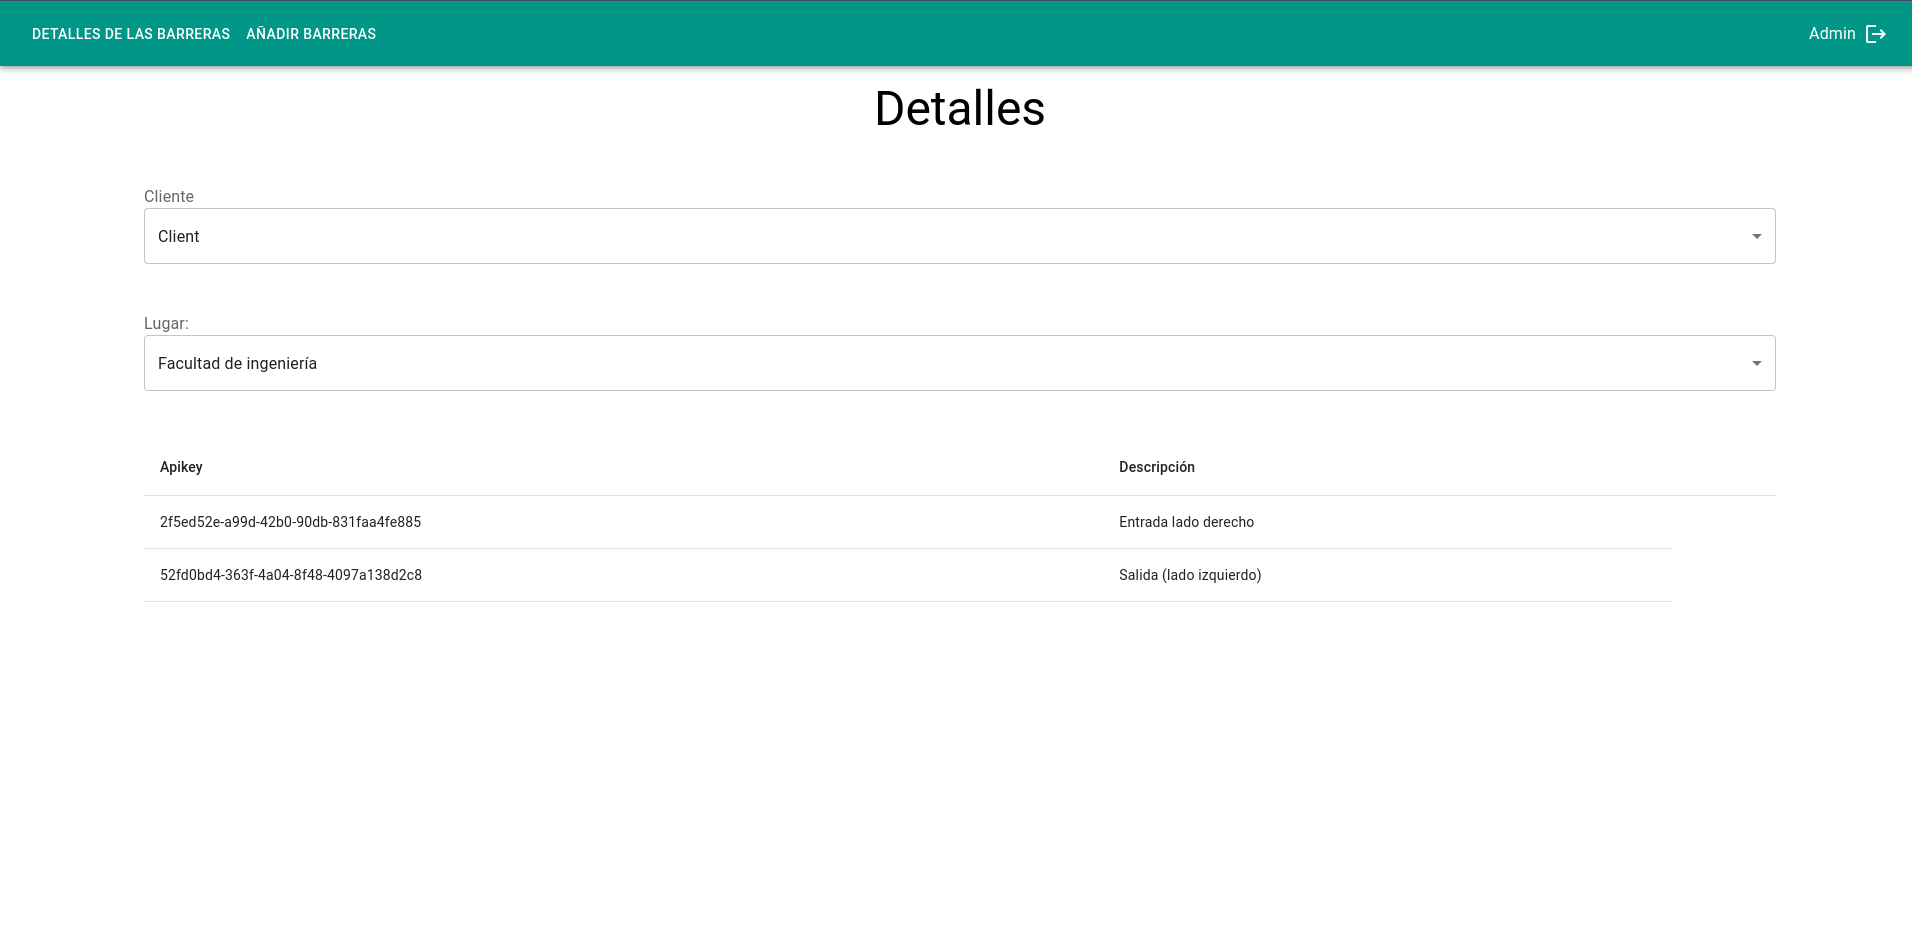
\includegraphics[width=\textwidth]{imgs/server/admin-details.png}
    \caption{Detalles de las barreras según cliente y estacionamiento.}
    \label{fig:admin-details}
\end{figure}

\begin{figure}
    \centering
    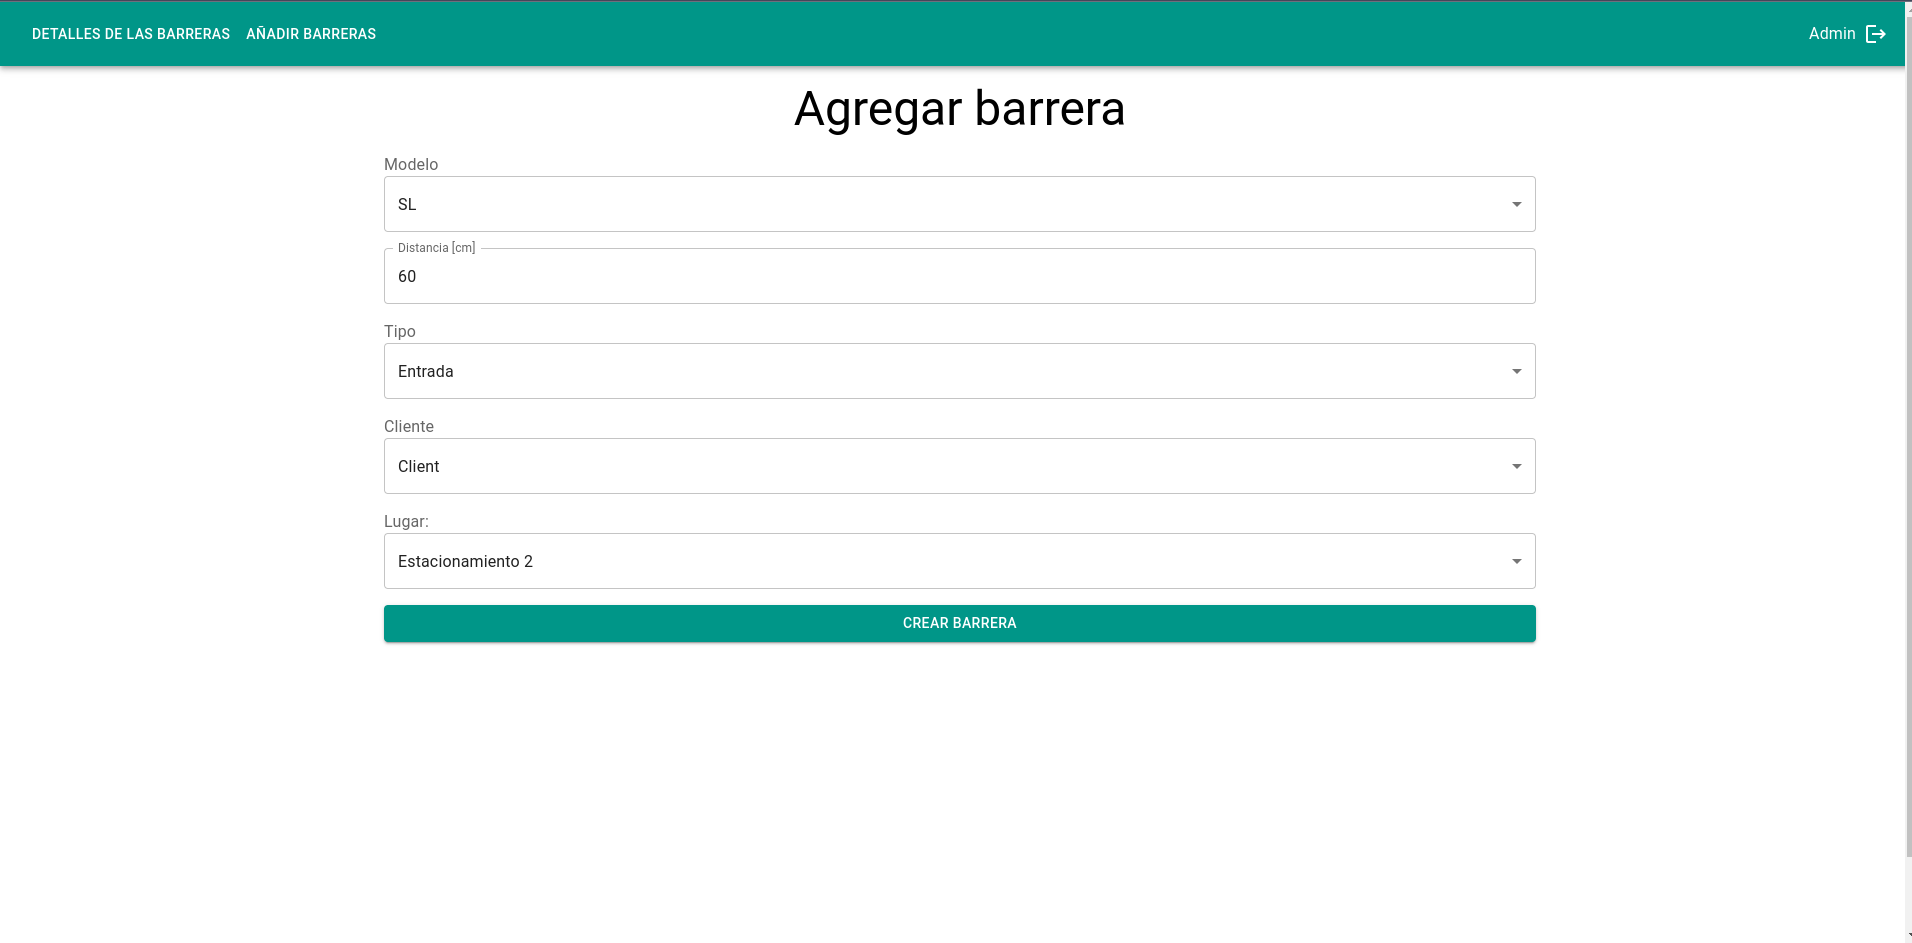
\includegraphics[width=\textwidth]{imgs/server/add-barrier.png}
    \caption{Formulario para agregar una barrera.}
    \label{fig:add-barrier}
\end{figure}

\subsection{Nginx}

Nginx es un servidor web de código abierto que permite la implementación de proxy inverso, cache de HTTP, y balanceo de cargo.
Su implementación se utiliza como proxy inverso entre el Backend y el Frontend.


\chapter{Pruebas de integración y fiabilidad}

El eje fundamental de este capítulo es mostrar el rendimiento del algoritmo y la integración final en diferentes circunstancias, y probar que el mismo es capaz de desenvolverse de forma satisfactoria en la mayoría de escenarios posibles.

\section{Pruebas sobre el algoritmo de OCR}
Para corroborar el funcionamiento del algoritmo se ensayaron diversas pruebas, con la finalidad de testear el comportamiento del algoritmo sobre diferentes entornos de trabajo, partiendo desde un ambiente ideal para llegar a uno alejado de él en el cual no se puede garantizar el correcto funcionamiento.

\subsection{Pruebas de distancia y ángulo}
Para realizar esta serie de pruebas se colocó un Volkswagen Up modelo 2015 con patente PEY232 en una posición fija y se procedió a medir con una cinta métrica de error 1 cm. Para las mediciones se consideró que la cámara y la patente están paralelas y enfrentadas. Este escenario define el ángulo de $0^\circ$ y cambia solamente cuando la cámara gira en dirección paralela al suelo, mientras que el origen se tomó desde el centro de la misma.
En Fig. \ref{fig:sistema-medicion-angulos} se puede apreciar un esquema del sistema de ejes. La medición consistió en la captura de una fotografía con la cámara de los sistemas SL a una distancia y ángulo determinados. Luego, cada medición se procesó con el algoritmo de OCR.
Debido al espacio con el que se contaba, se realizaron dos pruebas: la primera consistió en fijar el angulo en $0^\circ$ e ir tomando muestras cada 50cm, mientras que en la segunda se fijó la distancia en 50 cm y se vario el ángulo cada $30^\circ$.
Las muestras obtenidas para la primera prueba pueden verse en la Fig. \ref{fig:fotos-distancia} y los resultados obtenidos en la Tab. \ref{tab:resumen-distancia}, mientras que para la segunda prueba las muestras se observan en la Fig. \ref{fig:fotos-angulo} y los resultados en la Tab. \ref{tab:resumen-angulo}.


\begin{figure}[bth]
    \centering
    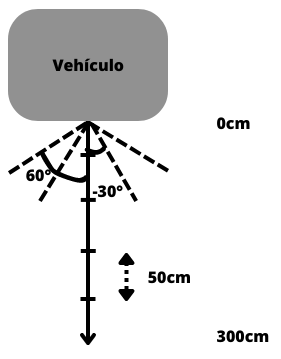
\includegraphics[width=.3\textwidth]{imgs/sistema-referencia.png}
    \caption{Sistema de referencia.}
    \label{fig:sistema-medicion-angulos}
\end{figure}

\begin{table}
    \centering
    \begin{tabular}{rl}
    \toprule
    Distancia & Predicción \\
    \midrule
    50        & PEY232     \\
    100       & PEY232     \\
    150       & PEY232     \\
    200       & PEY232     \\
    250       & PEY232     \\
    300       & PEY232     \\
    \bottomrule
\end{tabular}

    \caption{Resumen de la prueba de distancia a $0^\circ$ grados.}
    \label{tab:resumen-distancia}
\end{table}

\begin{table}
    \centering
    \begin{tabular}{rl}
    \toprule
    Ángulo & Predicción \\
    \midrule
    -60    & PEY232     \\
    -30    & PEY232     \\
    0      & PEY232     \\
    30     & PEY232     \\
    60     & PEY232     \\
    \bottomrule
\end{tabular}

    \caption{Resumen de la prueba de ángulos a 50 cm.}
    \label{tab:resumen-angulo}
\end{table}

\begin{figure}[bth]
    \centering
    \begin{subfigure}{.3\textwidth}
        \centering
        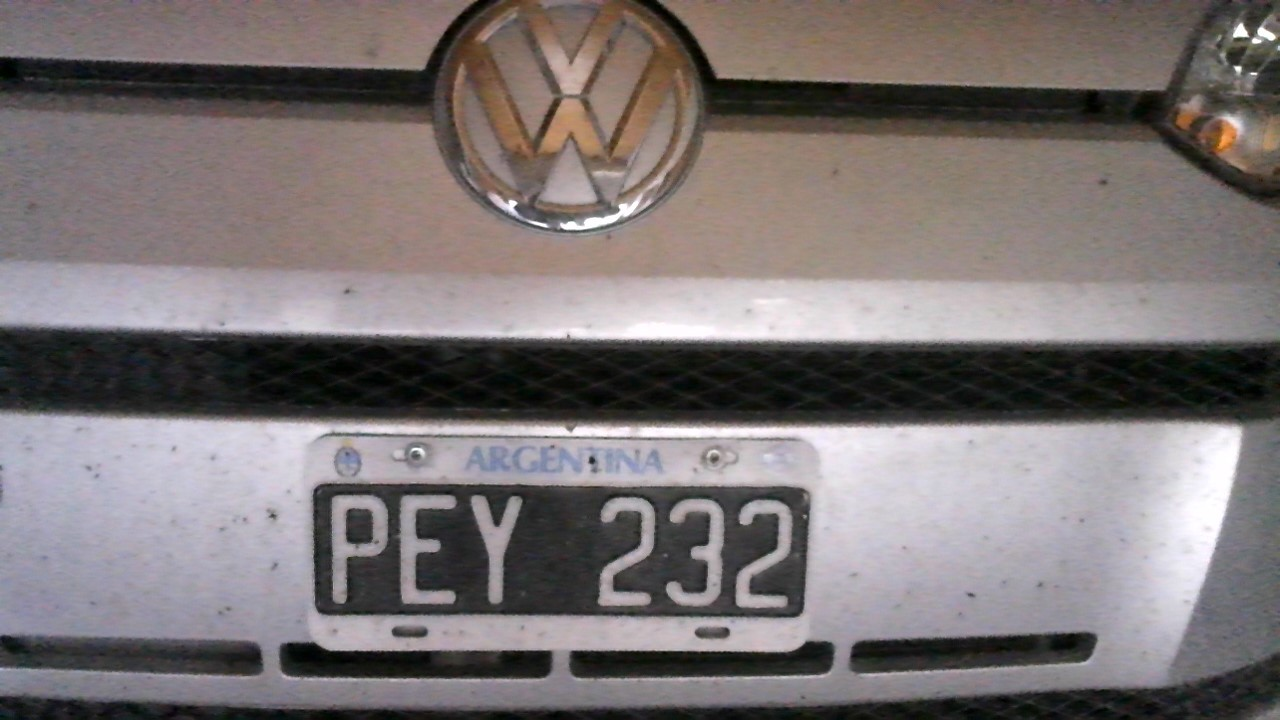
\includegraphics[width=\textwidth]{imgs/test-distancia/0_50.jpg}
        \caption{50cm}
    \end{subfigure}
    \begin{subfigure}{.3\textwidth}
        \centering
        \includegraphics[width=\textwidth]{imgs/test-distancia/0_100.jpg}
        \caption{100cm}
    \end{subfigure}
    \begin{subfigure}{.3\textwidth}
        \centering
        \includegraphics[width=\textwidth]{imgs/test-distancia/0_150.jpg}
        \caption{150cm}
    \end{subfigure}
    \begin{subfigure}{.3\textwidth}
        \centering
        \includegraphics[width=\textwidth]{imgs/test-distancia/0_200.jpg}
        \caption{200cm}
    \end{subfigure}
    \begin{subfigure}{.3\textwidth}
        \centering
        \includegraphics[width=\textwidth]{imgs/test-distancia/0_250.jpg}
        \caption{250cm}
    \end{subfigure}
    \begin{subfigure}{.3\textwidth}
        \centering
        \includegraphics[width=\textwidth]{imgs/test-distancia/0_300.jpg}
        \caption{300cm}
    \end{subfigure}
    \caption{Fotografías a diferentes distancias a $0^\circ$.}
    \label{fig:fotos-distancia}
\end{figure}

\begin{figure}[bth]
    \centering
    \begin{subfigure}{.15\textwidth}
        \centering
        \includegraphics[width=\textwidth]{imgs/test-angulos/-60_50.jpg}
        \caption{$-60^\circ$}
    \end{subfigure}
    \begin{subfigure}{.15\textwidth}
        \centering
        \includegraphics[width=\textwidth]{imgs/test-angulos/-30_50.jpg}
        \caption{$-30^\circ$}
    \end{subfigure}
    \begin{subfigure}{.15\textwidth}
        \centering
        \includegraphics[width=\textwidth]{imgs/test-angulos/0_50.jpg}
        \caption{$0^\circ$}
    \end{subfigure}
    \begin{subfigure}{.15\textwidth}
        \centering
        \includegraphics[width=\textwidth]{imgs/test-angulos/30_50.jpg}
        \caption{$30^\circ$}
    \end{subfigure}
    \begin{subfigure}{.15\textwidth}
        \centering
        \includegraphics[width=\textwidth]{imgs/test-angulos/60_50.jpg}
        \caption{$60^\circ$}
    \end{subfigure}
    \caption{Fotografías a diferentes ángulos a $50cm$.}
    \label{fig:fotos-angulo}
\end{figure}

\subsection{Pruebas de exterior}
Esta prueba se realizó con una cámara Kanon PowerShot SX150 IS \cite{kanon_powershot_nodate} en el ingreso al estacionamiento de la Facultad de Ingeniería de la Universidad Nacional del Comahue entre las 8 y 9 de la mañana, el martes 6 de junio del 2023. La prueba se realizó colocando la cámara en un trípode con una altura de 70cm respecto del suelo\footnote{Se consideran los 60cm del tripode y los 10cm de la calzada, debido a que no era conveniente colocar la cámara sobre la calle.}, y se procedió a filmar los vehículos que entraban al estacionamiento o circulaban por la calle interna Libres Pensadores de la universidad. De este proceso de medición se obtuvieron dos videos de una duración aproximada de 40min.

Teniendo en cuenta que el algoritmo de OCR tarda 1200ms en procesar un frame es necesario realizar un filtrado, ya que los 40min de filmación equivalen en 72000 imágenes, y la mayoría no poseen vehículos o la patente no está enfocada.
El proceso de filtrado consistió en un recorte manual de las partes del video donde no había ningún vehículo, lo que terminó dejando 7min de filmación. Si bien este número es bajo, llevó a obtener un total de 35 vehículos diferentes en distintos frames, suficientes para el análisis. Posteriormente se convirtió el video en frames, utilizando Open CV, para luego procesar las 11000 fotografías y eliminar en las que no era posible detectar la forma de una patente por un ser humano. Luego se obtuvieron 3600 fotografías, que se procesaron por el algoritmo de OCR y se descartaron todas las imágenes con porcentaje de confianza inferior al $50\%$. La confianza de la red sobre una patente estimada se define como el promedio de las probabilidades para cada carácter.

Las imágenes se clasificaron en una carpeta con el valor predicho por el algoritmo.
Finalmente se contabilizaron los errores generando el resumen de Tab. \ref{tab:resumen-patente}.

\begin{table}
    \centering
    \begin{tabular}{cccccccc}
    \toprule
    Caracteres & Perfectas & 1 error & 2 errores & 3 errores & 4 errores & 5 errores & $\sum$ \\
    \midrule
    6          & 60        & 78      & 25        & 10        & 3         & 0         & 176    \\
    7          & 282       & 185     & 49        & 5         & 1         & 1         & 523    \\
    $\sum$     & 342       & 263     & 74        & 15        & 4         & 1         & 699    \\
    \bottomrule
\end{tabular}

    \caption{Resumen de las patentes reconocidas.}
    \label{tab:resumen-patente}
\end{table}


\subsection{Análisis de resultados}

En base a las pruebas de interior, se logra apreciar que el rendimiento del algoritmo de OCR resulta satisfactorio en un entorno ideal controlado,  es decir en un escenario de vehículo detenido, corta distancia y un angulo entre $-60^\circ$ y $60^\circ$.
Por otro lado, en la prueba de exterior en la cual el escenario presenta condiciones extremas y no favorables, como velocidad no nula, distancia variable (corta, media y larga distancia) y ángulos fuera de rango, los resultados obtenidos cuentan con una baja eficiencia.


Realizando un análisis más exhaustivo de la prueba de exterior es posible obtener que la eficiencia del sistema ronda el $49\%$.
En la Tab. \ref{tab:resumen-patente} se observa que para patentes de seis caracteres la eficiencia ronda el $34\%$ esto se puede deber a que el dataset de entrenamiento contaba con una mayor tasa de patentes de siete caracteres o a que el estado de las patentes de seis caracteres al ser de mayor antigüedad se encuentran en peores condiciones lo que dificulta su estimación.
Por otro lado cuando se trata de patentes de siete caracteres estas poseen una eficiencia cercana al $54\%$, valor que se considera aceptable para esta prueba.
Se observa que para ambos casos la mayor tasa de error se da cuando existe un único carácter erróneo independientemente de su posición. Finalmente, es importante recordar que estos resultados se obtuvieron para un escenario poco favorable como los ejemplificados en la Fig. \ref{fig:collage-autos}. Si se extrapolan a un escenario menos hostil (vehículo cercano a la cámara y velocidad baja), los errores en la Tab. \ref{tab:resumen-patente} disminuirán considerablemente.

\begin{figure}[bth]
    \centering
    \includegraphics[width=\textwidth]{imgs/collage-autos.png}
    \caption{Ejemplificación de las imágenes obtenidas durante la prueba de exterior.}
    \label{fig:collage-autos}
\end{figure}

En base a estas pruebas se define que los limites para las condiciones de trabajo son:
\begin{enumerate}
    \item Distancia entre 50cm y 2m.
    \item Ángulo entre $-60^\circ$ y $60^\circ$.
    \item Velocidad de circulación paso de hombre.
\end{enumerate}
Los valores de distancia se toman teniendo en cuenta que el largo de un auto ronda los 4m \cite{duran_que_2023}, es por ello que se considera una distancia máxima de detección de 2m.
\section{Pruebas sobre el servidor}

\subsection{Integración de los sistemas SL y servidor}

Se montó un sistema SL mini junto con una notebook como servidor, el sistema montado se observa en la Fig. \ref{fig:pruebas-integracion-sl-server}, y se crearon registros de entrada, y cambio la configuración de un sistema SL en tiempo real. Con esta prueba se logró probar los cambios de configuración en tiempo real y que los registros se creen de forma correcta.

\begin{figure}
    \centering
    \begin{subfigure}[b]{.3\textwidth}
        \centering
        \includegraphics[width=\textwidth]{imgs/pruebas-integracion/server-sl.png}
    \end{subfigure}
    \begin{subfigure}[b]{.3\textwidth}
        \centering
        \includegraphics[width=\textwidth]{imgs/pruebas-integracion/sl-auto.png}
    \end{subfigure}
    \begin{subfigure}[b]{.3\textwidth}
        \centering
        \includegraphics[width=\textwidth]{imgs/pruebas-integracion/pruebas.png}
    \end{subfigure}

    \caption{Vistas del SL mini y servidor junto con el vehículo de durante las pruebas de integración.}
    \label{fig:pruebas-integracion-sl-server}
\end{figure}


\subsection{Creación de registros}

Para probar el correcto de funcionamiento del servidor, se creó un usuario de admin y un cliente. Se crearon dos lugares junto con un script en Python 3 emulando el envío de datos de las barreras, generando en el servidor 5900 registros para los lugares, probando el funcionamiento del sistema de inicio a fin los resultados de estas pruebas pueden observarse Fig. \ref{fig:dashboard}, algunos de los registros creados pueden apreciarse en la Fig. \ref{fig:registers}.

\section{Estado del prototipo}

En la actualidad se cuentan con 2 prototipos funcionales, uno para la versión SL y otro para el modelo SL mini.
El prototipo SL se encuentra montado sobre la placa Nvidia Jetson TX1 en su kit de desarrollo, la cual es capaz de correr el algoritmo de forma local.
Mientras que la versión SL mini se ejecuta en la placa Raspberry Pi 3 b+, que como se hizo mención en anterior capítulos no es capaz de correr el algoritmo de OCR por lo que esta tarea, se ejecuta en el servidor de prueba. El mismo se encuentra alojado en una notebook de la marca CX, la cual cuenta con un procesador Intel i5-1135G7, con 32 GB de ram, sin gpu dedicada, con lo que el tiempo de procesamiento por imagen es de 1,2s, como se mencionó en la Tab. \ref{tab:ocr}.
Para ambos modelos se cuenta con la misma cámara usb genérica y el sensor de distancia ultrasónico US-100.
Ambos prototipos se pueden apreciar en la Fig. \ref{fig:prototipos}.
\begin{figure}[bth]
    \begin{subfigure}{.45\textwidth}
        \centering
        \includegraphics[height=5cm]{imgs/prototipo-sl.jpeg}
        \caption{Prototipo SL.}
        \label{fig:prot-sl}
    \end{subfigure}
    \begin{subfigure}{.45\textwidth}
        \centering
        \includegraphics[height=5cm]{imgs/prototipo-sl-mini.jpeg}
        \caption{Prototipo SL mini.}
        \label{fig:prot-sl-mini}
    \end{subfigure}
    \caption{Prototipos en su estado actual.}
    \label{fig:prototipos}
\end{figure}



\chapter{Conclusiones}
En este capítulo se realizarán las conclusiones generales correspondientes al uso de redes neuronales convolucionales para el uso de detección de caracteres, más específicamente para detectar patentes argentinas, se detallarán las ventajas y desventajas encontradas en los algoritmos, para finalmente presentar posibles mejoras a futuro.

\section{Conclusiones generales}

Durante el proceso de investigación sobre OCR y sus utilidades, se observó que en nuestro país este tipo de tecnologías son poco explotadas, con aplicaciones escasas, limitándose al uso de herramientas creadas por terceros.
Por lo que el diseño de este prototipo representa una innovación en lo que a control de acceso de estacionamientos respecta, permitiendo una automatización y control del acceso de los vehículos al recinto con una interacción nula por parte del usuario.

Se ha estudiado en profundidad el funcionamiento de redes neuronales, más específicamente las CNN y se observó que estas son las más favorables para la implementación en sistemas embebidos, por su bajo costo computacional en comparación con las LSTM, logrando reconocer las patentes de manera efectiva.

Uno de los enfoques más importantes de este trabajo fue el diseño modular, buscando que la interdependencia de las partes del sistema sea lo más baja posible, es decir, permite cambiar partes del sistema disminuyendo los errores al integrar estos nuevos elementos.
Por ejemplo, es posible cambiar el servicio de detección de patentes por uno mejor, sin necesidad de cambiar el código del back-end o del front-end, respetando solo que la comunicación entre el back-end y este servicio sea por HTTP y devuelva el JSON esperado.
A su vez este diseño permite cambiar el sensor de distancia o la cámara sin tener un gran impacto en el resto del sistema.
En síntesis este tipo de diseño permite una mayor flexibilidad a la hora de integrar nuevas tecnologías.

En general las tareas de diseño y desarrollo son complejas, sobre todo a la hora de brindar soluciones innovadoras.
Sin embargo se logró desarrollar un prototipo funcional para permitir el acceso de vehículos a un estacionamiento sin interacción de los usuarios.

\section{Posibles mejoras}
Finalmente se presentan posibles mejoras en los sistemas de obtención de imágenes, detección y obtención de caracteres estudiados a lo largo de este trabajo:
\begin{itemize}
    \item Implementar un nuevo algoritmo para la detección de patentes en otro tipo de vehículos (motos, camiones).
    \item Mejorar la eficiencia del algoritmo de OCR.
    \item Desarrollar e implementar de algoritmo de reconocimiento de patentes extranjeras.
    \item Reducir el costo de ensamble de los sistemas SL.
    \item Sustituir la cámara por una que permita mejores fotografías en ambientes externos.
    \item Integrar una pasarela de pagos para efectuar el cobro del estacionamiento.
    \item Desarrollar una versión con display para mejorar la experiencia de los usuarios.
\end{itemize}


\printbibliography
\end{document}